% Bachelor Thesis Webperformance für den mobilen Endanwender
% von Andreas Lorer
% 2015
% Studiengang: Angewandte Informatik - HS Ravensburg-Weingarten
\documentclass[a4paper,11pt,singlespacing]{article}
\usepackage[left=2.5cm,right=2.5cm,top=2.5cm]{geometry}
\usepackage[hyphens]{url}
\usepackage[backend=biber,style=alphabetic,backref=true,citecounter=true,citestyle=authoryear]{biblatex}
\usepackage{csquotes}
\usepackage{hyperref}
\usepackage{setspace}
\usepackage{csquotes}
\usepackage[utf8]{inputenc}
\usepackage[T1]{fontenc}
\usepackage[ngerman]{babel}
\usepackage{color}
\usepackage{hyperref}
\usepackage{pdflscape}
\usepackage{graphicx}
\usepackage{listings}
\usepackage{longtable}
\usepackage{array}
\usepackage{fancyhdr}
\addbibresource{sections/zitate.bib}
\pagestyle{empty}
\author{Andreas Lorer}

\graphicspath{{images/}
}\setlength{\parindent}{0ex}  	% Absatzeinrueckung verhindern

\definecolor{materialGrey}{rgb}{0.27,0.27,0.27}
\definecolor{materialGreen}{rgb}{0.0, 0.8, 0.6}
\definecolor{materialRed}{rgb}{0.82, 0.1, 0.26}
\definecolor{materialYellow}{rgb}{1.0, 0.5, 0.0}
\definecolor{materialBlue}{rgb}{0.0, 0.5, 1.0}
\definecolor{lightgray}{rgb}{.9,.9,.9}
\definecolor{darkgray}{rgb}{.4,.4,.4}
\definecolor{purple}{rgb}{0.65, 0.12, 0.82}

\begin{document}
  % document styles for listings
  \lstset{
    backgroundcolor=\color{white},
    basicstyle=\footnotesize\ttfamily,
    breakatwhitespace=true,
    breaklines=true,
    numbers=left,
    numbersep=5pt,
    deletekeywords={event}, 
    numberstyle=\tiny,
    showspaces=false,
    showtabs=false,
    language=html,
    keywordstyle=\bfseries\color{materialRed},
    commentstyle=\itshape\color{materialGreen},
    columns=fullflexible,
    xleftmargin=0.5cm,
    xrightmargin=1cm,
    frame=lr,
    framesep=8pt,
    framerule=0pt
  }

\lstdefinelanguage{JavaScript}{
  keywords={typeof, new, true, false, catch, function, return, null, catch, switch, var, if, in, while, do, else, case, break, length},
  keywordstyle=\color{materialBlue}\bfseries,
  ndkeywords={class, export, boolean, throw, implements, import, this},
  ndkeywordstyle=\color{darkgray}\bfseries,
  identifierstyle=\color{black},
  sensitive=false,
  comment=[l]{//},
  morecomment=[s]{/*}{*/},
  commentstyle=\color{purple}\ttfamily,
  stringstyle=\color{materialRed}\ttfamily,
  morestring=[b]',
  morestring=[b]"
}

\lstset{
   language=JavaScript,
   backgroundcolor=\color{lightgray},
   extendedchars=true,
   basicstyle=\footnotesize\ttfamily,
   showstringspaces=false,
   showspaces=false,
   numbers=left,
   numberstyle=\footnotesize,
   numbersep=9pt,
   tabsize=2,
   breaklines=true,
   showtabs=false,
   captionpos=b
}
\lstset{literate=%
   *{0}{{{\color{materialYellow}0}}}1
    {1}{{{\color{materialYellow}1}}}1
    {2}{{{\color{materialYellow}2}}}1
    {3}{{{\color{materialYellow}3}}}1
    {4}{{{\color{materialYellow}4}}}1
    {5}{{{\color{materialYellow}5}}}1
    {6}{{{\color{materialYellow}6}}}1
    {7}{{{\color{materialYellow}7}}}1
    {8}{{{\color{materialYellow}8}}}1
    {9}{{{\color{materialYellow}9}}}1
}
	%Deckblatt
  \newcommand{\headline}{Bachelor-Thesis}
  \newcommand{\subheadline}{Web Performance für den mobilen}
  \newcommand{\subsubheadline}{Endanwender}
	\begin{titlepage}
  \begin{center}

    % Upper part of the page
    
\includegraphics[width=0.5\textwidth]{../deckblatt/images/logo.png}\\[2cm]    
    {\huge \bfseries \headline}\\[0.5cm]
    {\huge \bfseries \subheadline}\\[0.5cm]
    {\huge \bfseries \subsubheadline}\\[0.5cm]
    
   % Zusammenfassung
    \begin{abstract}
      \noindent
       \\[1cm]
    \end{abstract}

    {\large \today}\\[1cm]
    \vspace{2cm}

	\begin{flushleft}
      \hspace*{3cm} Columbus Interactive\\
      \hspace*{3cm} Eywiesenstraße 6\\
      \hspace*{3cm} 88212 Ravensburg\\
      \vspace{1cm}
      \hspace*{3cm} Fakultät Elektrotechnik und Informatik\\
      \hspace*{3cm} Studiengang Angewandte Informatik\\
      \hspace*{3cm} Hochschule Ravensburg-Weingarten\\
      \hspace*{3cm} Doggenriedstraße, 88250 Weingarten

    \end{flushleft}

    \vspace{1.5cm}

    % Authoren
    \begin{flushleft}\large
	  \hspace*{2cm} \emph{Autor:}\\
	  \hspace*{2cm} Andreas Lorer\\
	  \hspace*{2cm} \href{mailto:andreas.lorer@hs-weingarten.de}{\nolinkurl{andreas.lorer@hs-weingarten.de} }\\
      \hspace*{2cm} 88250 Weingarten\\
      \hspace*{2cm} Wilhelmstraße 4
    \end{flushleft}
   \end{center}
   \vfill
\end{titlepage}

  \begin{titlepage}
  \begin{center}

    \vspace{5.5cm}
    % Upper part of the page
    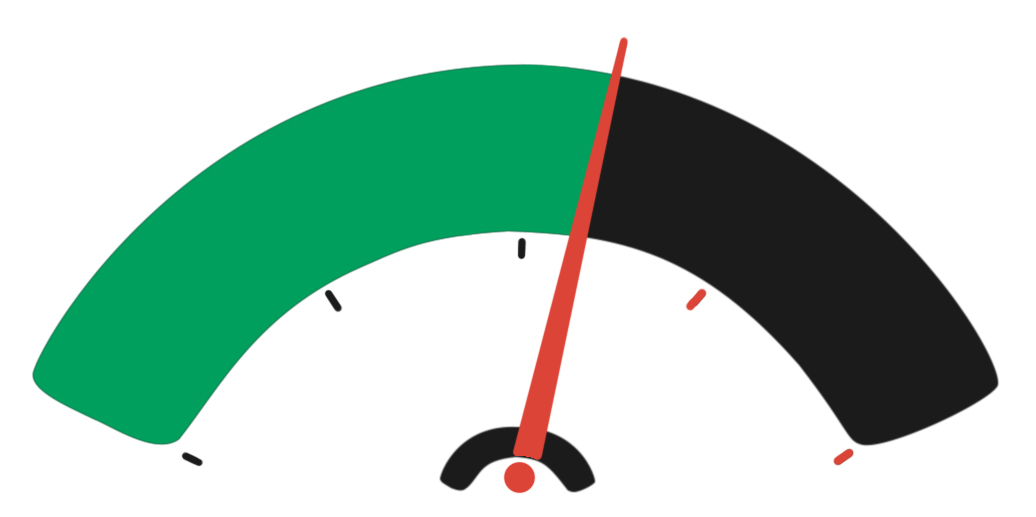
\includegraphics[width=0.6\textwidth]{../deckblatt/images/webperf_logo.jpg}\\[3cm]    
    {\huge \bfseries \headline}\\[1.5cm]
    {\huge \bfseries \subheadline}\\[0.5cm]
    {\huge \bfseries \subsubheadline}\\[0.5cm]
  \end{center}
\end{titlepage}

	
	%Inhaltsverzeichnis
  \thispagestyle{empty}
	\tableofcontents 
  \clearpage
  \pagestyle{fancy}
  \fancyhf{}
  % \rhead{}
  \lhead{Web Performance für den mobilen Endanwender}
  \rfoot{\thepage}
  \renewcommand{\headrulewidth}{0.4pt}
  \renewcommand{\footrulewidth}{0.4pt}

  \setcounter{page}{1}

\section{Einleitung} % (fold)
\label{sec:einleitung}
	Diese Arbeit beschäftigt sich umfassend mit dem Thema Web Performance unter dem Aspekt, dass immer mehr Anwender mittels Smartphone mit dem Web agieren. Sie soll die Frage klären, warum Webanwendungen auf einem Smartphone oftmals um ein Vielfaches langsamer Laden, als via Desktop-PC, welche Auswirkungen sich daraus ergeben und welche Maßnahmen zur Optimierung ergriffen werden können. Daraus resultiert ein \texttt{Workflow}, der sich nach den "`Best Practices"' richtet. Die Arbeit endet mit den kulturellen Veränderungen, die das Thema Web Performance für ein Unternehmen mit sich bringen kann und welche Herausforderungen es zu meistern gilt.

	\subsection{Motivation} % (fold)
	\label{sub:motivation}

		Niemand mag es, zu warten. Sei es auf Bus, Bahn oder an der Kasse im Supermarkt. Wir warten auch nicht gerne im Internet auf das Buffern eines Videos, beim Besuch einer Webseite oder beim Shoppen via App. Zu oft wird aus dem "`nur mal eben diesen Begriff nachschlagen"' ein endloses Starren auf den weißen Bildschirm. Jeder kennt das.\\

		Larry Page, CEO und Mitgründer von Google, sagt:
		\begin{quote}
			\textit{"`As a product manager you should know that speed is the number one feature."'}\autocite{holzle10}
		\end{quote}
		Niemand mag es, zu warten, auch nicht auf eine Webanwendung. Die Studie "`The Psychology of Web Performance"' zitierte bereits im Jahr 2008 folgende Ergebnisse:

		\begin{quote}\itshape
			"`Slow web pages lower perceived credibility and quality. Keep your page load times below tolerable attention thresholds, and users will experience less frustration, lower blood pressure, deeper flow states, higher conversion rates, and lower bailout rates. Faster websites are actually perceived to be more interesting and attractive."' \autocite{webOpti08}
		\end{quote}

		Das Hauptvermarktungsargument für den Chrome Browser war damals, er sei schneller als die Konkurrenz. Tatsächlich ist für Google Geschwindigkeit alles. Deshalb hat Google im Jahr 2010 angekündigt, dass Geschwindigkeit in die Berechnung des \texttt{Google Page Rankings} mit einfließt.

		\begin{quote}\itshape
			"`Faster sites create happy users and we've seen in our internal studies that when a site responds slowly, visitors spend less time there. [...] Recent data shows that improving site speed also reduces operating costs. Like us, our users place a lot of value in speed — that's why we've decided to take site speed into account in our search rankings"'\autocite{google10}
		\end{quote}

		Aktuell (2015) geht Google sogar noch einen Schritt weiter und informiert tausende Webmaster per E-Mail über die schlechte Usability ihrer Websites für mobile Besucher und warnt ausdrücklich vor dementsprechend "`angepassten Rankings"'.\autocite{t3n15}
		Im Hinblick auf die Zukunft wird der Marktanteil an mobilen Internetnutzern noch weiter wachsen und die Optimierung der Ladezeiten gewinnt dadurch noch mehr an Bedeutung. Zwischen 2011 und 2014 stieg die Anzahl der Smartphonenutzer von 18\% auf 50\% an. Dies ist ein Wachstum von 32\% innerhalb von nur 3 Jahren.\autocite{tns14}\\

		\begin{figure}[htbp]
			\begin{center}
				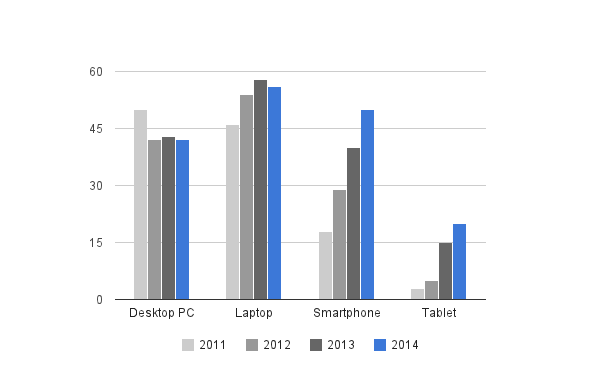
\includegraphics[width=0.75\textwidth]{smartphoneUsage.png}
			\end{center}
			\caption{Gerätenutzung in der Gesamtbevölkerung (2011 – 2014)\autocite{tns14}}
			\label{fig:geraetenutzung}
		\end{figure}

		Die Antwort auf diesen Trend läutete eine Ära ein, die wir heute unter dem Namen \texttt{Responsive Webdesign} kennen. "`Responsive"' muss aber sehr viel mehr bedeuten, als nur eine angepasste Darstellung für eine bestimmte Art von Gerät. \textit{"`Two out of three mobile shoppers expect pages to load in 4 seconds or less."'} \autocite{radware13}. Der Anwender erwartet also auf dem Smartphone ähnliche oder gleiche Ladezeiten wie er sie auch von der Nutzung des Desktop Pc's gewohnt ist. Diese Erwartungen werden von dem Großteil der Internetseiten nicht erfüllt. Der Inhalt einer Seite muss darum so aufbereitet werden, dass dieser auch auf Geräten mit langsamer Internetverbindung, hoher Latenz und einem begrenzten Datentarif, in einer für den Anwender annehmbaren Geschwindigkeit, angezeigt werden kann.\\

	% subsection motivation (end)



	\subsection{Zielsetzung} % (fold)
	\label{sub:zielsetzung}
		Um gängige Methoden und Techniken der Ladezeit-Optimierung anzuwenden, wird das Projekt anhand der Website \url{http://andreaslorer.de/old/} durchgeführt. Das Ziel ist es, die Ladezeit der Website auf dem Smartphone, wie auch auf dem Desktop auf unter 1000 Millisekunden zu verringern. Mit Ladezeit ist dabei nicht die Zeit gemeint, die benötigt wird, um die Website komplett zu laden, sondern die Zeit, bis eine erste visuelle Rückmeldung für den Anwender zu sehen ist. Diese, vom Anwender wahrgenommene Rückmeldung, nennt man auch "`Perceived Performance"' und bedeutet, dass die Ladezeit als schneller empfunden wird, als es eigentlich laut Messwerten der Fall ist. Näheres dazu wird in Punkt \ref{sub:perceived_performance} beschrieben.\\

	% subsection zielsetzung (end)



	\subsection{Eigene Leistung} % (fold)
	\label{sub:eigene_leistung}
		Die Leistung besteht darin, einen Gesamtüberblick über die heutigen Best Practices zu ermöglicht. Die Arbeit soll dem Leser ein Gespühr für Fehler in der Struktur von Webanwendungen geben, die für die Geschwindigkeit hinderlich sind.
		Es soll herausgefunden werden, was getan werden muss um die Ladezeit zu minimieren, wie ein moderner "`Workflow"' aussehen kann, damit eine Webanwendung schon bei seiner Entstehung schnell lädt und im Projektverlauf schnell bleibt. Des Weiteren soll erklärt werden, welche Herausforderungen es zu meistern gilt um eine schnelle Webanwendung zu erreichen, welche Tools es gibt und welche Vor- oder Nachteile diese mit sich bringen.\\
		Diese Arbeit befasst sich nicht mit der Geschwindigkeit von Datenbanken, SQL-Abfragen oder sonstigen Problemen, die durch einen Engpass ein schnelles Laden der Seite verhindern könnten.

	% subsection eigene_leistung (end)



	\subsection{Ist-Zustand} % (fold)
	\label{sub:ist_zustand}
		Die Webseite \url{www.andreaslorer.de}  ist auf einem \texttt{Shared Hosting}
		\footnote{Bei shared Hosting werden mehrere Websites von verschiedenen Website-Betreibern von dem gleichen Webserver gehostet. Bei Shared Hosting teilen sich in der Regel Hunderte andere Websites einen Server \autocite{itWissen}} 
		aufgesetzt und die Antwortzeit des Servers beträgt circa <200 Millisekunden. Dadurch, dass es keine Möglichkeit gibt, \texttt{Root Rechte}\footnote{Standardmäßig existiert unter Linux immer ein Konto für den Benutzer "`root"' mit der User-ID 0. Dies ist ein Systemaccount mit vollem Zugriff auf das gesamte System, und damit auch auf alle Dateien und Einstellungen aller Benutzer \autocite{ubuntu14}} auf einem Shared Hosting zu bekommen, können so manche serverseitige Einstellungen nicht durchgeführt werden. Diese werden dann zwar aufgezeigt, kommen aber für dieses Projekt nicht zum Einsatz.\\
		Die Website hat als Ausgangsbasis einen einfachen Aufbau. Sie besteht aus einer Bilder Gallerie basierend auf PHP und dem Bootstrap Framework.
	% subsection ist_zustand (end)



\pagebreak
%
% section einleitung (end)
%

  
\section{Begriffe}
\label{sec:begriffe}
	\subsection{Pattern und Antipattern} % (fold)
	\label{sub:pattern_und_anti_pattern}
		"`Entwurfsmuster (englisch design patterns) sind bewährte Lösungsschablonen für wiederkehrende Entwurfsprobleme sowohl in der Architektur als auch in der Softwarearchitektur und -entwicklung. Sie stellen damit eine wiederverwendbare Vorlage zur Problemlösung dar, die in einem bestimmten Zusammenhang einsetzbar ist."'\autocite{pattern15}
		\\

		"`Während "`Design Patterns"' in der Software-Entwicklung allgemein übliche und bekannte Ansätze sind, um Probleme zu lösen, sind Anti-Patterns Negativ-Beispiele – die zeigen, wie man es nicht macht - von bereits durchgeführten, gescheiterten Projekten, die dem erkennenden Mitarbeiter zielgerichtete Hinweise darauf geben, wie die Aufgabenstellung besser gelöst werden könnte. Als Synonym ist auch der Begriff Negativmuster im Gebrauch. Es ist tatsächlich möglich, daß das, was gestern noch als allgemein gangbarer Lösungsweg bezeichnet wurde, heute schon ein "`Antipattern"' ist [...]"' \autocite{Stepken06}

	% subsubsection pattern_und_anti_pattern (end)

	

	\subsection{TCP Three Way Handshake}
	\label{sub:tcp_three_way_handshake}
		TCP ist das meistgenutzte Verbindungsprotokoll im Internet. Auf diesem Protokoll wird der HTTP Request aufgebaut, der die eigentlichen Daten enthält.
		Bevor Daten zwischen Server und Browser ausgetauscht werden können, muss eine Verbindung aufgebaut werden. Abbildung ~\ref{fig:three_way_handshake} beschreibt den Prozess des Verbindungsaufbaus.\footnote{Für ein tieferes Verständnis empfiehlt sich dieser Artikel: \href{http://chimera.labs.oreilly.com/books/1230000000545/ch02.html}{High Performance Browser Networking - Chapter 2: Building Blocks of TCP}} 

		\begin{figure}[htbp]
			\begin{center}
				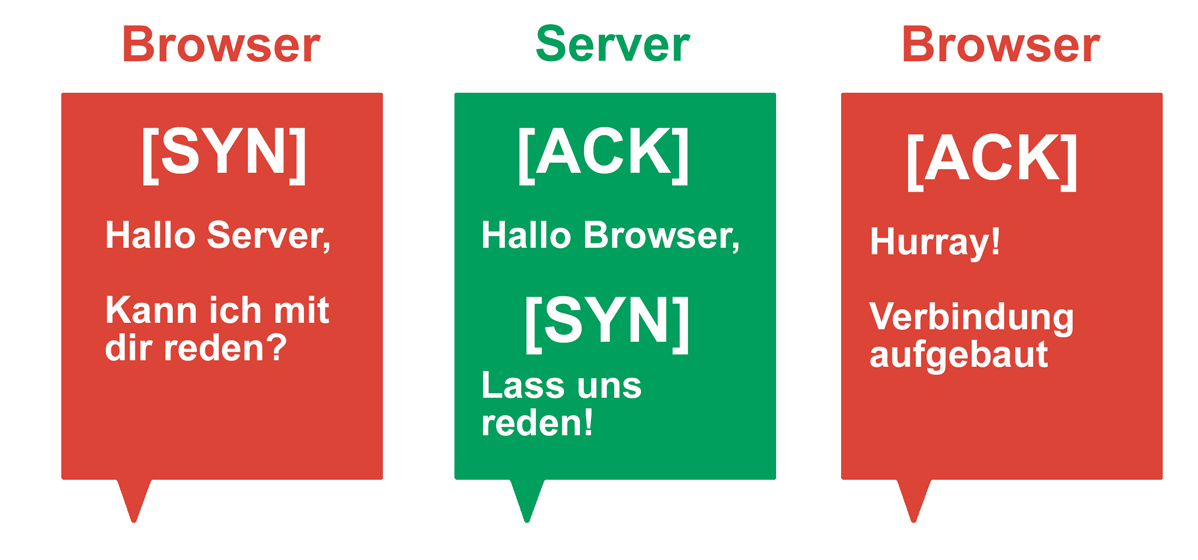
\includegraphics[width=0.6\textwidth]{three_way_handshake.jpg}
				\caption{Three-Way-Handshake zum Aufbau einer TCP Verbindung zwischen Browser und Server (Eigene Abbildung nach: \autocite{bos})}
				\label{fig:three_way_handshake}
			\end{center}
		\end{figure}
	% subsection tcp_three_way_handshake (end)

	\subsection{Latenz} % (fold)
	\label{sub:latenz}
		Latenz bezeichnet die Verzögerung, bis ein Paket von Sender A zu Empfänger B gelangt ist.
	% subsection latenz (end)


	\subsection{Round Trip Time (RTT)} % (fold)
	\label{sub:round_trip_time_}
		"`Round Trip Time"' wird im Deutschen Paketumlaufzeit genannt. Es bezeichnet die Zeit die ein Datenpaket braucht um in einem Netzwerk von Sender A zu Empfänger B und wieder zurück zu gelangen. Bei einer Latenz von 100ms würde die RTT folglich 200ms betragen (Annahme: Hin- und Rückweg haben die selbe Zeit).
	
	% subsection round_trip_time_ (end)

	\subsection{TCP Slow Start} % (fold)
	\label{sub:tcp_slow_start}

		Ein Round Trip kann nicht beliebig viele Bytes transportieren sondern ist durch die sogenannte "`Congestion Window Size"'\footnote{engl. congestion: Stauung, Überlastung, Anhäufung} limitiert. Der Überbegriff für dieses Verhalten nennt sich "`Slow Start"'

		\begin{figure}[htbp]
			\begin{center}
				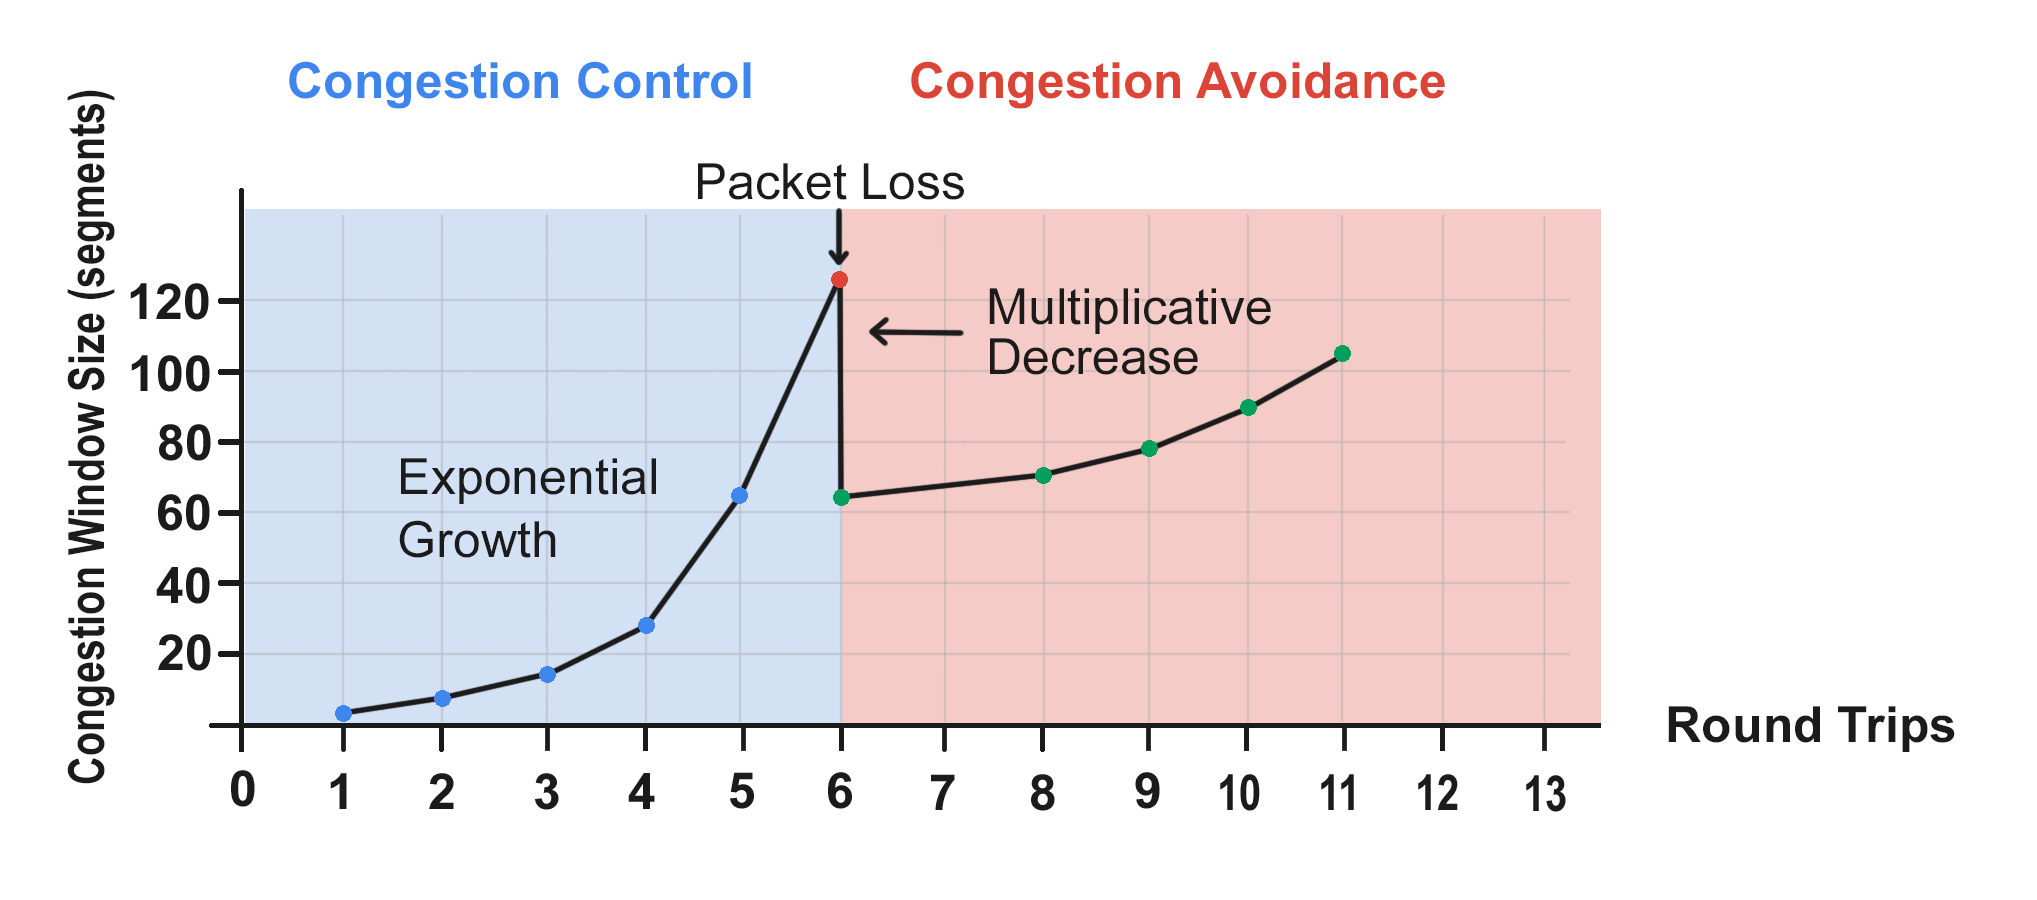
\includegraphics[width=\textwidth]{congestion_window_size.jpg}
				\caption{Congestion Control und Congestion Avoidance (Eigene Abbildung nach \autocite{grigorikSlowStart})}
				\label{fig:congestion_window_size}
			\end{center}
		\end{figure} 

		\begin{itemize}
			\item Congestion Control: Nach dem eine neue Verbindung per TCP aufgebaut wurde, können weder Server noch Client wissen, wie schnell die Verfügbare Bandbreite ist, mit der Daten ausgetauscht werden können. Um das Netzwerk, vor einem Datenstau zu schützen, wird mit einem sehr niedrigen Wert begonnen, der dann ansteigt bis das Limit erreicht ist. Dieses Verhalten nennt sich auch "`Congestion Control"' und verhindert das Aufstauen von Daten.
			\item Congestion Window Size: Diese Größe bestimmt, wieviel Bytes der pro Segmente geschickt werden darf, bis diese vom Empfänger per \texttt{ACK} (acknowledgement) bestätigt werden müssen. Die Größe der Segmente ist Standardmäßig 1460 bytes und die Rate bis zum ACK ist im April 2013 von 4 auf 10 Segmente erhöht worden.\autocite{grigorikSlowStart}. In der Grafik wird davon ausgegangen, das der erste Round Trip 4 Segmente senden darf. Die Datenrate Wächst exponentiell an, damit möglichst schnell die volle Bandbreite nutzbar ist.\\
			\item Congestion Avoidance bedeutet, dass sich die Datenrate wieder um ein Vielfaches verringert, falls es zu einem Paketverlust kommt. Da es besonders bei WLAN oder Mobilfunknetzen des öfteren zu Packetverlusten kommen kann ist dieser Aspekt besonders hervorzuheben, denn er verzögert das erreichen der maximal möglichen Datenrate.
		\end{itemize}

		Slow Start bedeutet also aus sicht der Performance, dass bei einer neuen TCP Verbindung nicht die maximale Bandbreite zu Verfügung steht. Bei größeren Dateien wird zwar durch das exponentielle Wachstum das Maximum schnell erreicht, gerade aber bei kleineren Dateien mit wenigen Kilobyte ist dies oft nicht der Fall.

	% subsubsection tcp_slow_start (end)


	\subsection{Content Delivery Network (CDN)} % (fold)
	\label{sub:content_delivery_network}
		Ein Content Delivery Network (CDN), oder auch Content Distribution Network genannt, ist ein Netz lokal verteilter und über das Internet verbundener Server, mit dem Inhalte ausgeliefert werden.\\
		CDN-Knoten sind auf viele Orte verteilt um Anfragen (Requests) von End-Nutzern nach Inhalten (Content) möglichst ökonomisch zu bedienen.\\
		Große CDNs unterhalten tausende Knoten mit zehntausenden Servern.\autocite{wikipediaCDN}

		\begin{figure}[htbp]
			\begin{center}
				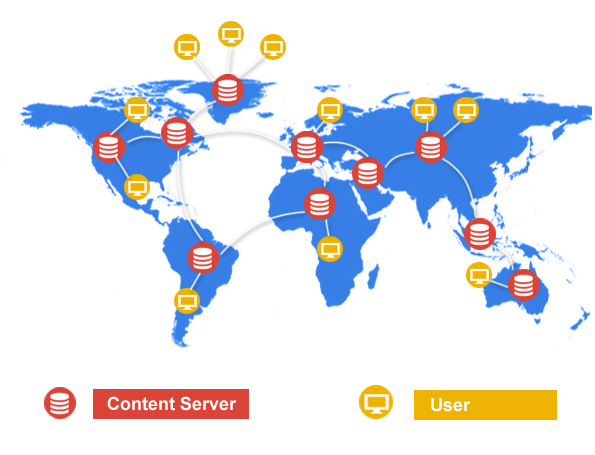
\includegraphics[width=0.6\textwidth]{cdn_network.jpg}
				\caption{Schematische Darstellung eines CDN (Eigene Abbildung nach \autocite{ritz14})}
				\label{fig:cdn_network}
			\end{center}
		\end{figure}
		
	% subsection content_delivery_network (end)


	\subsection{Above The Fold} % (fold)
	\label{sub:above_the_fold}
		Damit ist der auf einem Bildschirm sichtbare Bereich vor dem Scrollen gemeint. Diesem Bereich wird eine besondere Wichtigkeit zugesprochen.
		\begin{figure}[htbp]
			\begin{center}
				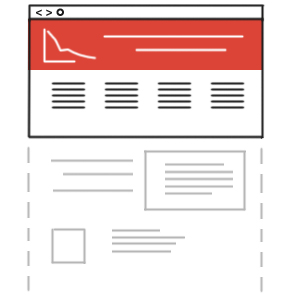
\includegraphics[width=0.3\textwidth]{above_the_fold.jpg}
				\caption{Darstellung des sichtbaren Bereichs vor dem Scrollen}
				\label{fig:above_the_fold}
			\end{center}
		\end{figure}

		\begin{quote}
			 \textit{"`In an analysis of 57,453 eyetracking fixations, we found that there was a dramatic drop-off in user attention at the position of the page fold. Elements above the fold were seen more than elements below the fold: the 100 pixels just above the fold were viewed 102\% more than the 100 pixels just below the fold."'} \autocite{nng15}
		\end{quote}

		Wichtige Informationen oder Navigationselemente sind meistens dort zu finden. Eine Webseite die nach dem Paradigma des Responsive-Webdesign aufgebaut ist kann dabei 3 oder mehrere Ansichten haben die alle einen unterschiedlichen "`above the fold"' bereich haben. Eine Anwendung kann aber auch unterschiedliche Seiten haben, auf dem der Anwender beim Aufrufen der Seite landen kann. Zum Beispiel wenn dieser An- oder Abgemeldet ist. Paradebeispiel dafür sind Facebook oder Twitter.

	% subsubsection above_the_fold (end)



	\subsection{Perceived Performance} % (fold)
	\label{sub:perceived_performance}
		\begin{figure}[htbp]
			\begin{center}
				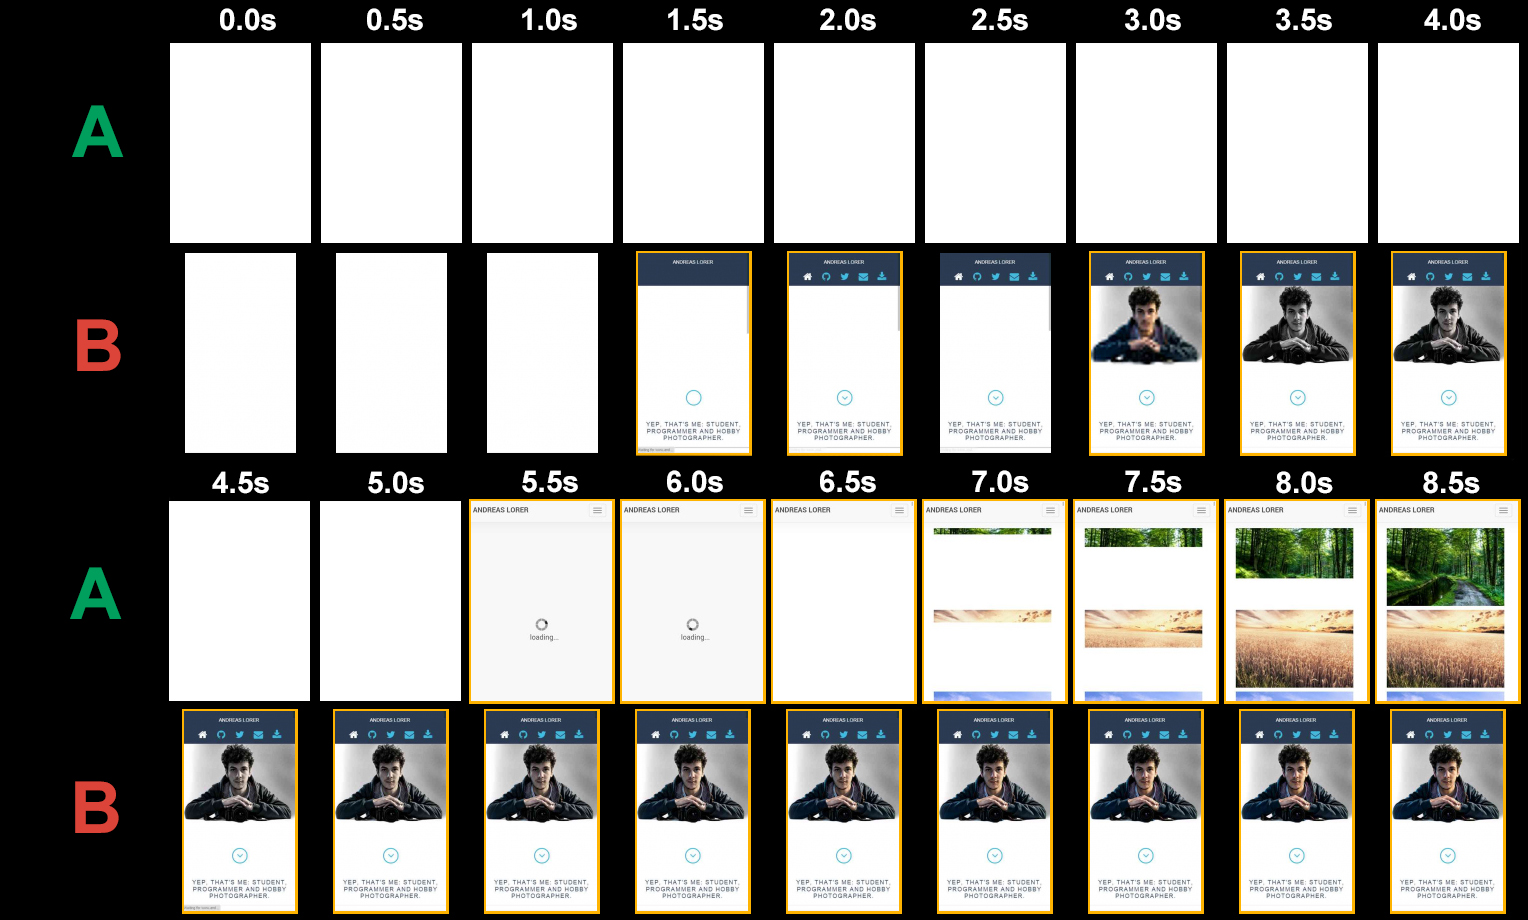
\includegraphics[width=0.9\textwidth]{perceived_performance.jpg}
				\caption{Zwei Seiten im Vergleich (Eigene Abbildung via webpagtest.org)}
				\label{fig:perceived_performance}
			\end{center}
		\end{figure}

		Abbildung \ref{fig:perceived_performance} zeigt die Seiten A und B, mit nahezu identischer Ladezeit. Der Unterschied besteht darin, dass Seite B bereits nach 1.5 Sekunden eine erste visuelles Rückmeldung für den Anwender zu sehen ist wohingegen Seite A erst nach 5.5 Sekunden dem Anwender zeigt, dass sie überhaupt ladet.
		"`Perceived Performance"' steht also für die Zeit bis ein erste visuelle Rückmeldung für den Anwender zu sehen ist und bedeutet, dass die Ladezeit als schneller empfunden wird, als es eigentlich laut Messwerten der Fall ist. Warum diese "`Perceived Performance"' für eine Webanwendung so wichtig ist zeigen mehrere Studien, deren Daten in folgender Infographik aufbereitet sind.

		\begin{figure}[htbp]
			\begin{center}
				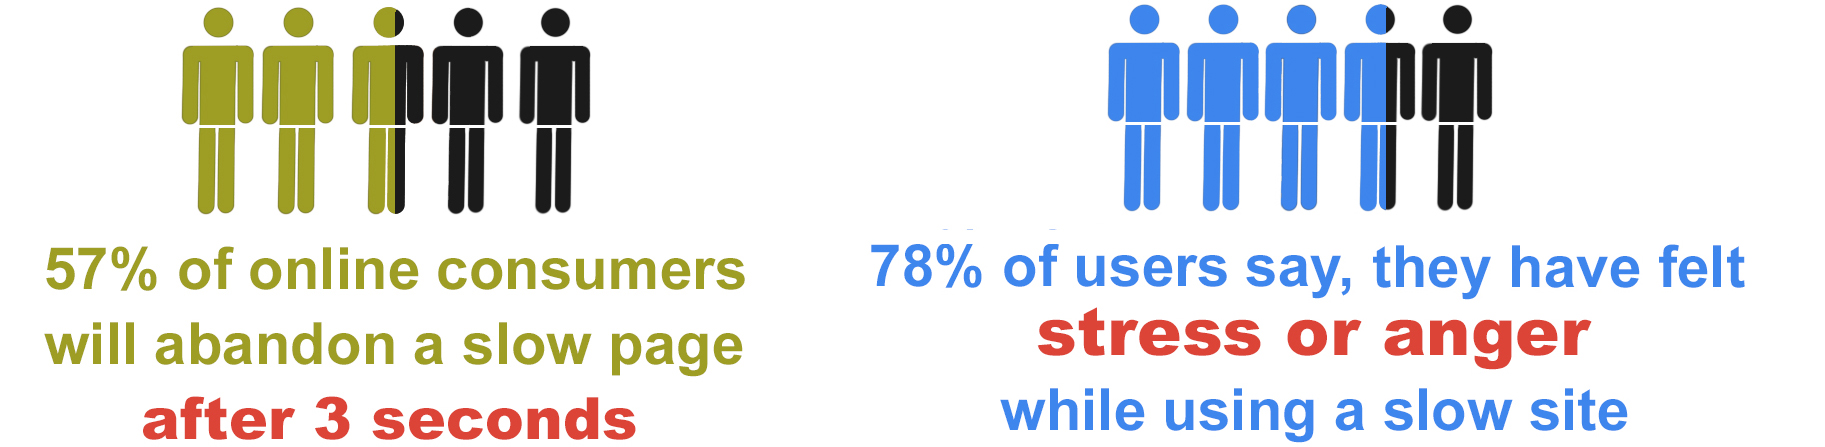
\includegraphics[width=0.7\textwidth]{effect_of_slow_loadtimes.jpg}
				\caption{Einfluss und Effekt einer langsamen Seite auf den Anwender (Eigene Abbildung nach Daten von: \autocite[p. 8]{radware14})}
				\label{fig:effect_of_slow_loadtimes}
			\end{center}
		\end{figure}

		Bereits kleine Verbesser- oder Verschlechterungen der Ladezeit können einen großen Einfluss in auf den Anwender haben. Yahoo hat herausgefunden, dass wenn eine Seite um nur 400 Millisikunden schneller ist, sich der Traffic um 9\% erhöhte.\autocite{stefanov08} 57\% der Online Konsumenten haben eine Seite, die länger als 3 Sekunden ladet bereits wieder verlassen. 78\% der Anwender empfinden sogar Zorn oder Stress wenn eine Seite nicht Ladet oder dies nicht ersichtlich ist.

	% subsubsection perceived_performance (end)
	\pagebreak
% subsection begriffe (end)



\section{Die 1000 ms Barriere} % (fold)
\label{sec:die_1000_ms_barriere}
	Das Ziel dieser Arbeit, die 1000 Millisekunden Barriere zu durchbrechen, wurde nicht durch einen Zufall gewählt. Der Anwender nimmt die Geschwindigkeit einer Seite subjektiv wahr. Sie wird in der folgenden Grafik interpretiert:

	\begin{figure}[htbp]
		\begin{center}
			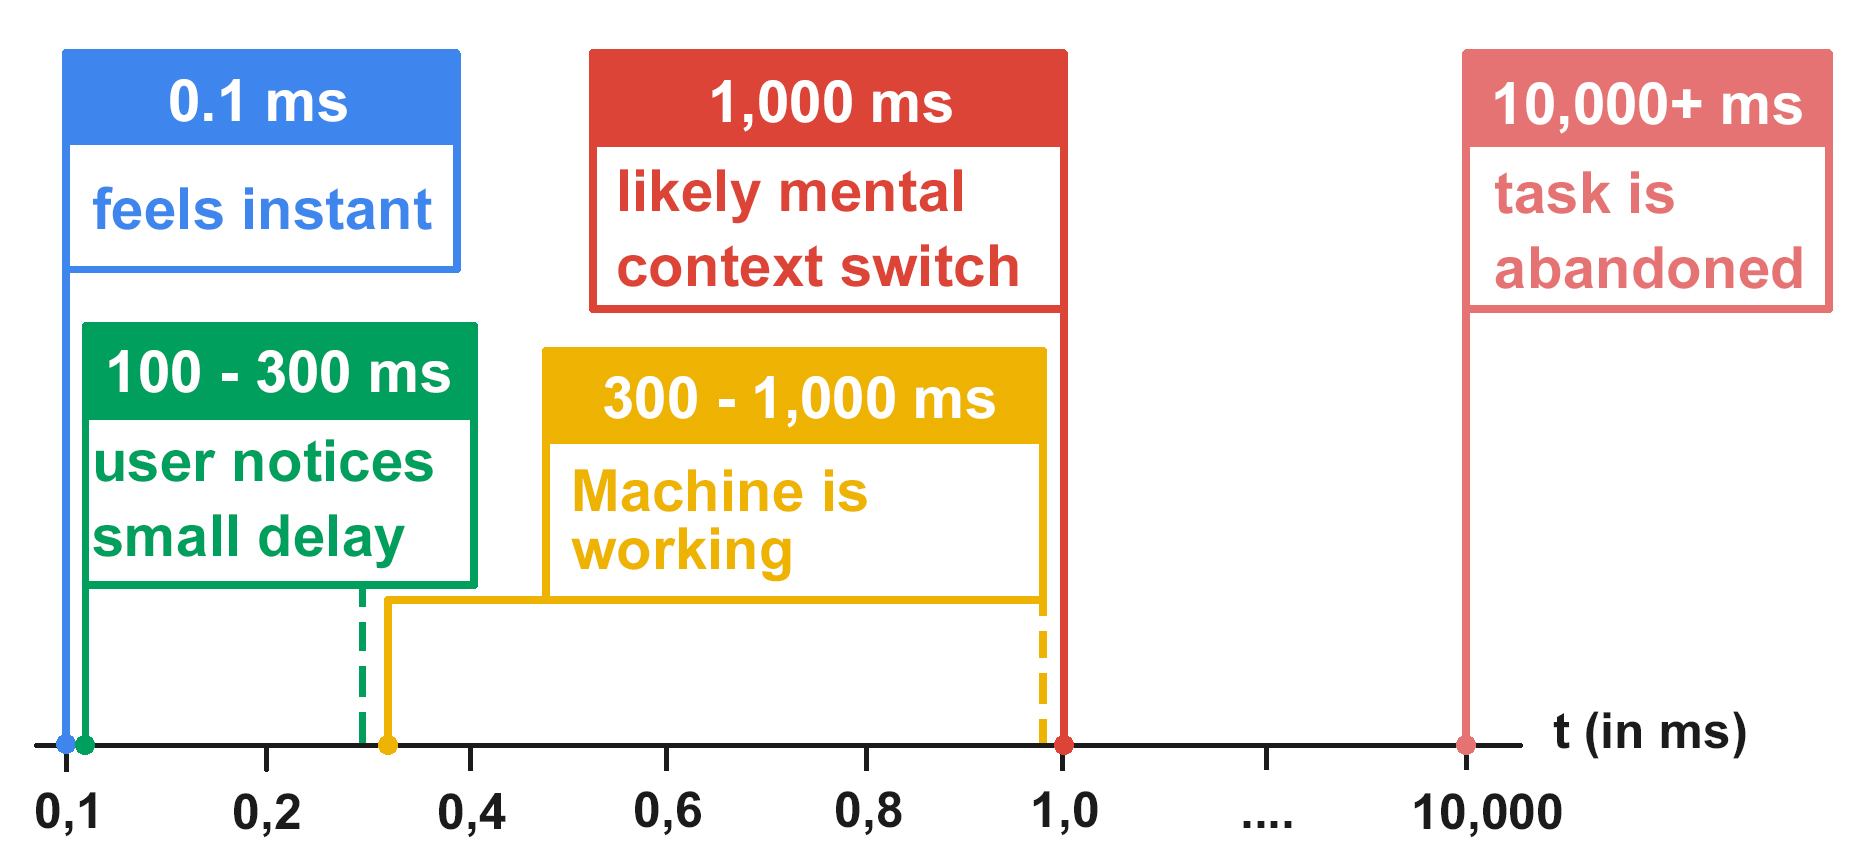
\includegraphics[width=\textwidth]{human_perception.jpg}
			\caption{Zeit und Wahrnehmung durch den Anwender (Eigene Abbildung nach Daten von: \autocite{grigorikHumanPerception})}
			\label{fig:human_perception}
		\end{center}
	\end{figure}

	Wie zu sehen ist bleiben gerade einmal eine Sekunde, bevor das Gehirn uns sagt, man solle doch einer anderen Aufgabe nachgehen bis der Ladevorgang abgeschlossen ist. Der Anwender verlangt visuelle Rückmeldung um "`am Ball zu bleiben"', dies wurde bereits in Punkt ~\ref{sub:perceived_performance} "`Perceived Performance"' angesprochen. Auf vielen Webseiten sieht man deshalb, Ladebalken oder sogenannte \texttt{Spinner}, die dem Anwender sagen, dass der Ladevorgang in gange, aber noch nicht abgeschlossen ist.

	Um das Ziel von einer Sekunde Ladezeit bis zum ersten Render zu erreichen, ist es nötig zu verstehen womit die meiste Zeit beim Aufrufen einer Webanwendung verbracht wird. Bevor eine Seite mittels Smartphone vom Browser dargestellt wird läuft eine ganze Reihe von Prozessen ab.



	\subsection{Touch Event} % (fold)
	\label{sub:touch_event}
		Der Aufruf einer Seite über das Smartphone erfolgt über ein Touch Event auf einen Link, Button oder die Seite wird per URL aufgerufen. Hierbei können je nach Gerät zwischen 50 (IPhone 5) und 123 Millisekunden (Moto X - Android) zwischen der Berührung des Touch Screen und dem Registrieren des Events vergehen.\autocite{venturebeat} Der Browser wartet allerdings nochmals bis zu 300 Millisekunden, denn er muss abwarten ob vielleicht noch ein zweiter Finger aufgelegt wird, oder ob der Anwender Scrollen oder Zoomen möchte.\autocite{google11}

		Dieses Verhalten lässt sich bei vielen Browsern per \texttt{Meta Tag} abstellen:

		\begin{lstlisting}
			<meta name="viewport" content="user-scalable=no">
		\end{lstlisting}

		Dies setzt natürlich voraus, dass die Webanwendung kein Zoomen benötigt um sie zu bedienen! Gerade bei älteren Webseiten trifft das oftmals nicht zu, da sie keine für das Smartphone angepasste Ansicht haben (responsive view). Eine vollständige Liste mit Meta Tags für die verschiedenen Browser ist der Fußnote zu entnehmen.\footnote{Suppressing 300ms delay for touchscreen interactions: \url{http://tinyurl.com/psj5nxz}}

	% subsection touch_event (end)

	\subsection{Netzwerke} % (fold)
	\label{sub:netzwerke}
		Warum gerade das nutzen des Internets per Smartphone so langsam sein kann (und oftmals ist) liegt zu einem Großteil am Netzwerk. Eine Studie untersuchte die Top eine Millionen Webseiten des Internets auf ihre Ladezeiten. Dabei wurde eine Verbindung von 5 Mbit/s und 28ms RTT benutzt. Eine RTT von 28 ms ist sehr schnell, vergleicht man sie zum Beispiel mit der Latenz des 3G Netzes (Abbildung ~\ref{fig:mobile_networks}). Diese Studie kam zu dem Ergebnis, dass fast 70\% der Ladezeit nur durch warten auf das Netzwerk verbracht wird:

		\begin{figure}[htbp]
			\begin{center}
				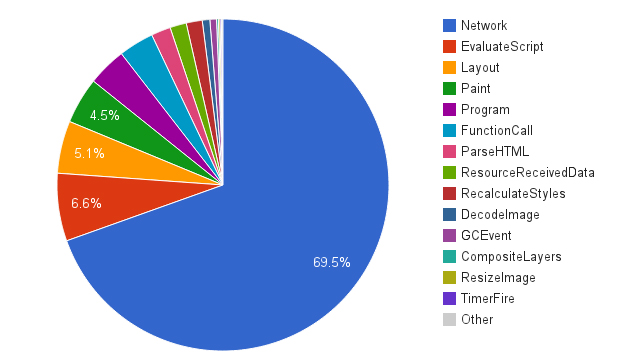
\includegraphics[width=0.8\textwidth]{time_on_network.jpg}
				\caption{Untersuchung der top 1 Millionen Alexa Seiten (Abbildung von: \autocite{alexa})}
				\label{fig:time_on_network}
			\end{center}
		\end{figure}

		Es macht also durchaus Sinn, sich diesen Bereich näher anzusehen, um zu verstehen worauf Einfluss genommen werden kann und wo nicht.


		\subsubsection{Mobilfunknetz} % (fold)
		\label{ssub:Mobilfunknetz}
			Es gibt unterschiedliche Mobilfunktsandards mit denen Anwender Anbindung an das Internet erlangen. Aber selbst wenn einem Anwender 4G vom Mobilfunkanbieter versprochen wird, so ist die Netzabdeckung mit 4G noch nicht vollständig deckend. Das bedeutet, dass der Anwender auf ein niedrigeres Netz wie zum Beispiel 3G ausweichen muss. Die verschiedenen Netzwerke unterscheiden sich entscheidend in ihrer Datenrate und vor allem in der Latenz. Folgende Tabelle gibt eine Übersicht:

			\begin{figure}[htbp]
				\begin{center}
					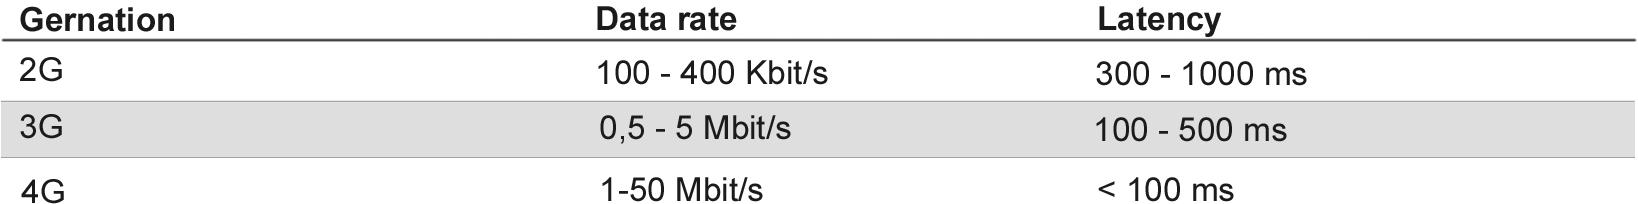
\includegraphics[width=\textwidth]{mobile_networks.jpg}
					\caption{Datenrate und Latenz für eine aktive mobile Verbindung (Eigene Abbildung nach Tabelle \autocite{grigorikGNetwork})}
					\label{fig:mobile_networks}
				\end{center}
			\end{figure}

			Unser Smartphone ist nicht ständig mit dem "`wireless service provider"' verbunden. Ist eine erste Verbindung nötig, so muss das Smartphone dem Sendeturm mitteilen, dass es Kommunizieren möchte. Der Anbieter muss die Anfrage Authentifizieren, die Verbindung herstellen und dann die Anfrage in das Internet weiter leiten. Die Zeit bis eine Authentifizierung erfolgt ist, kann je nach Anbieter und Mobilfunkstandard zwischen <100ms (LTE) und 2,5 Sekunden (3G) liegen \autocite{grigorikRadio}! Bereits hier ist zu sehen, dass es "`worst case"' Szenarien gibt, durch die es nicht möglich sein kann, dass eine Webanwendung unter einer Sekunde eine Rückmeldung gibt. Gerade Mobilfunknetze unterliegen Stoßzeiten, die Funksignale von Smartphones können sich gegenseitig stören oder das Signal kann in gewissen Gegenden stärker oder schwächer sein.

		% subsubsection Mobilfunknetz (end)


		\subsection{Der HTTP-Request} % (fold)
		\label{sub:der_http_request_komponente}
			Nachdem uns unser Mobilfunkanbieter mit dem Internet verbunden hat, kann die eigentliche Anfrage an den Server gestellt werden.

			\begin{figure}[htbp]
				\begin{center}
					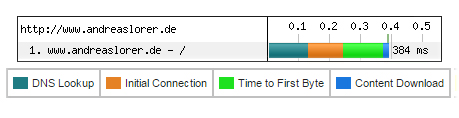
\includegraphics[width=0.8\textwidth]{http_components.jpg}
					\caption{Anfrage der HTML-Datei von Irland mittels 3G Netz (Abbildung nach \url{http://webpagetest.org})}
					\label{fig:http_components}
				\end{center}
			\end{figure}

			\begin{itemize}
				\item DNS Lookup: Um eine Verbindung mit dem Server herzustellen benötigt das HTTP Protokoll die IP Adresse des Ziels. Das heißt der DNS Server wird für den Namen "`http://andreaslorer.de"' die zu diesem Namen zugehörige IP Adresse zurückgegeben.

				\item Initial Connection bezeichnet die Zeit die vergeht, bis eine neue Verbindung zum Server hergestellt wurde damit eine Kommunikation zwischen Browser und Server stattfinden kann. Hierbei findet der sogenannte TCP "`Three-Way-Handshake"' statt, der dafür einen Round Trip benötigt.

				\item TTFB: Ist die Abkürzung für "`Time to first byte"'. Dieser Begriff beschreibt die Zeit die vergeht, bis das erste Byte vom Server beim Browser ankommt. Der Server muss den Request erst zusammenstellen bevor er ihn versenden kann. Dafür werden unter umständen Daten aus der Datenbank abgefragt oder es müssen berechnungen stattfinden. Diese Faktoren beeinflussen die TTFB und kann optimiert werden (schnellerer Server, bessere Datenbankanbindung, Caching).

				\item Content Download: Die Zeit die benötigt wird bis die Datei vom Server Heruntergeladen wurde.

				\item Nachdem das HTML Dokument heruntergeladen wurde, muss es vom Browser noch gelesen und interpretiert werden. Diese Zeit taucht im Diagramm nicht auf.
			\end{itemize}
					
		% subsection http_request_komponente (end)
	% section netzwerke (end)

	\subsection{Das Herunterladen einer 40 KB Datei} % (fold)
	\label{sub:das_herunterladen_einer_40_kb_datei}

		Abbildung ~\ref{fig:fetching_40kb} zeigt Schematisch wie eine 40 KB Datei mittels einer neuen TCP Verbindung heruntergeladen wird. Sie soll verdeutlichen, wie vor allem die RTT eine entscheidende Rolle spielt und warum die Latenz die Geschwindigkeit einer Seite viel höher beeinflusst als die Bandbreite.

		\begin{figure}[htbp]
			\begin{center}
				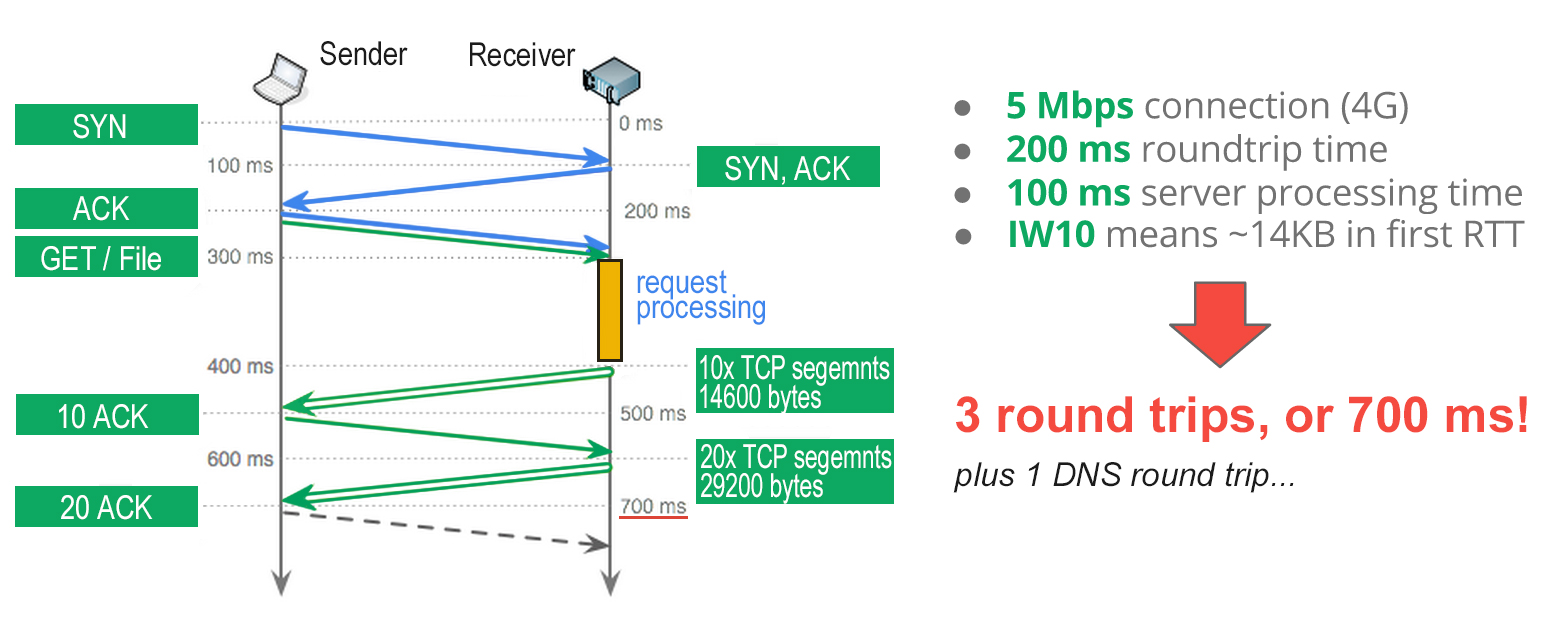
\includegraphics[width=\textwidth]{fetching_40kb.jpg}
				\caption{Herunterladen von 40KB mittels TCP (Abbildung nach \autocite{grigorikTCP})}
				\label{fig:fetching_40kb}
			\end{center}
		\end{figure}

		Zuerst erfolgt der DNS Lookup, dann muss TCP per \texttt{three way handshake} eine Verbindung aufbauen. Dies kostet bereits 2 round trips, was in diesem Beispiel 400 ms entspricht.
		Durch den TCP slow start (siehe Punkt: ~\ref{sub:tcp_slow_start} TCP slow start) steht bei einer neuen TCP Verbindung nicht die volle Bandbreite zur Verfügung. Deshalb kann die volle Datenmenge nicht auf einmal, sondern nur durch zusätzliche round trips heruntergeladen werden. Wenn die Performance einer Webanwendung verbessert werden soll, macht es also Sinn in round trips zu denken. Wieviel round trips sind nötig, bis ich dem Browser informationen übermittelt habe, so dass dieser etwas anzeigen kann? 
		
		\begin{figure}[htbp]
			\begin{center}
				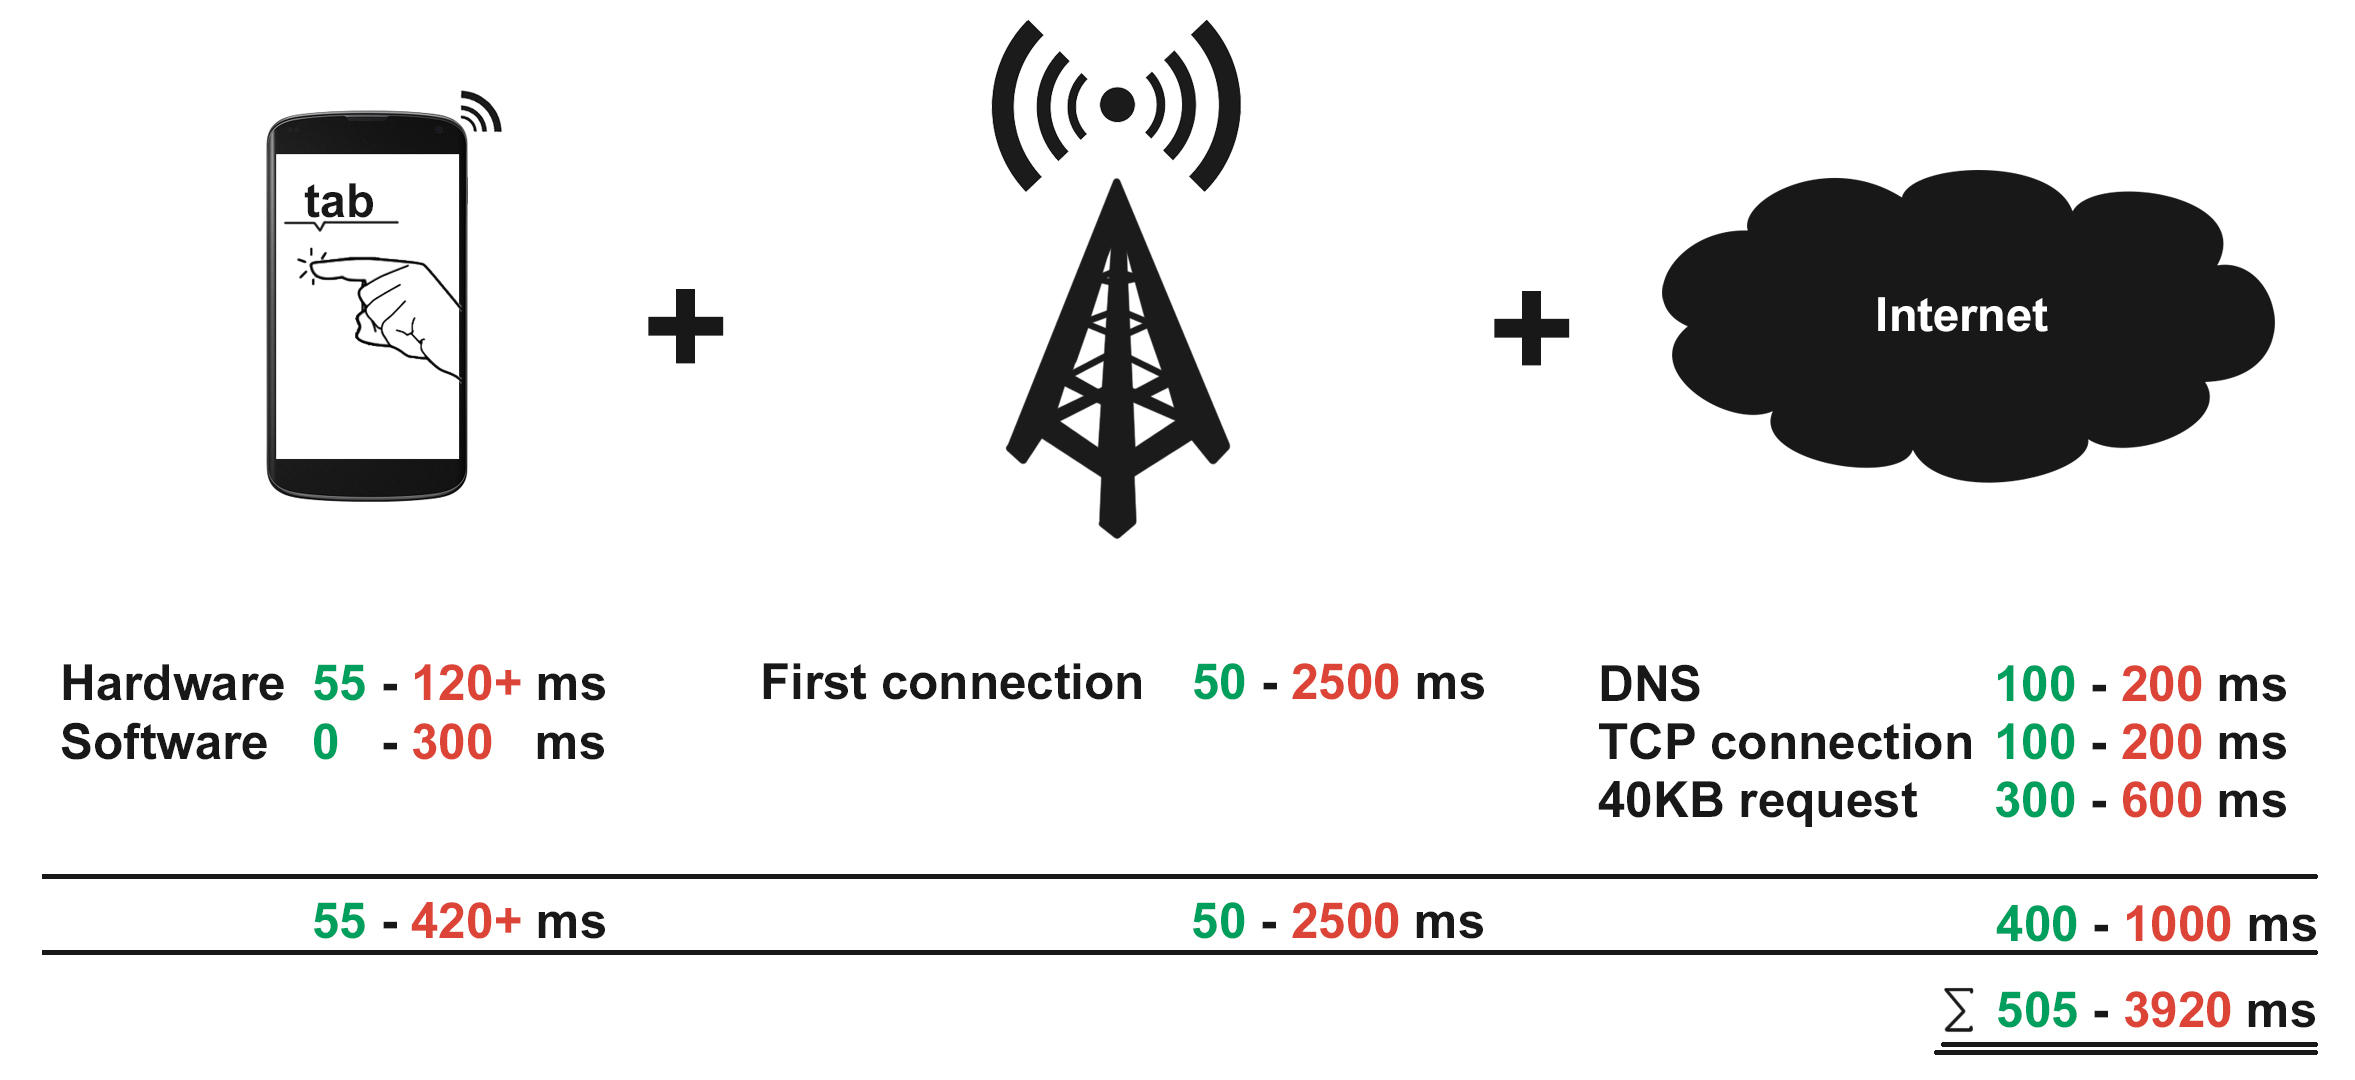
\includegraphics[width=0.9\textwidth]{1000ms_budget.jpg}
				\caption{1000 ms Budget (Eigene Abbildung)}
				\label{fig:1000ms_budget}
			\end{center}
		\end{figure}

		Wie in Abbildung ~\ref{fig:1000ms_budget} zu sehen ist bleibt von dem 1000 Millisekunden Budged nicht mehr viel übrig, wenn man alleine die Netzwerkzeiten abzieht. Im "`best case"' Szenario bleiben knapp 500 ms.
		Das bedeutet es müssen in den ersten Kilobytes, soviel nützliche Informationen vorhanden sein, damit der Browser bereits anfangen kann mit dem rendering zu beginnen, obwohl noch nicht alle Daten heruntergeladen sind. Noch spitzer formuliert: Der Browser sollte mit den ersten 14 KB (das ist die Menge an Daten die der erste round trip transportieren kann, siehe Abbildung ~\ref{fig:fetching_40kb}) bereits den \texttt{above the fold} bereich rendern können. Um das zu ermöglichen ist es nötig, den Kritischen Rendering-Pfad zu optimieren.
		
	% subsection das_herunterladen_einer_40_kb_datei (end)

	\subsection{Zusammengefasst} % (fold)
	\label{sub:zusammengefasst}
		Folgende Optimierungsmaßnahmen ergeben sich auf der Ebene des Netzwerks:
		\begin{itemize}
			\item Näheres Platzieren der Bits: Die Latenz bestimmt vorrangig die Geschwindigkeit des Ladevorgangs. Durch die benutzung eines CDN's lassen sich Bits und Bytes näher am Endanwender platzieren.
			\item Sage das Nutzerverhalten vorraus: Wenn der Anwender in einer Einkaufs-App 3 Schritte zum vollenden des Kaufvorgangs benötigt, dann lässt sich bei Schritt 1 bereits vorhersagen was er für weitere Ressourcen im nächsten Schritt benötigt. Diese Ressourcen könnten bereits geladen werden.
			\item Wahl eines guten Hostings: Die RTT als auch die \texttt{Server Response Time} sind je nach Anbieter unterschiedlich. Ein gutes Hosting kann hier unter umständen bereits eine enorme Verbesserung bedeuten. Zur not sollte gewechselt werden!

			\begin{figure}[htbp]
				\begin{center}
					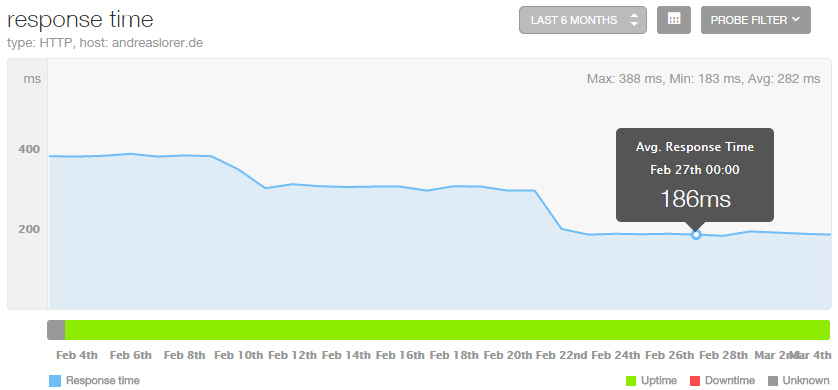
\includegraphics[width=0.9\textwidth]{choose_a_good_host.jpg}
					\caption{Verringerung der response time für http://andreaslorer.de (Abbildung nach pingdom.com)}
					\label{fig:choose_a_good_host}
				\end{center}
			\end{figure}
			
			Wie in der Grafik zu sehen ist, sank die Response Zeit meines Hosting Providers von durchschnittlichen fast 400 Millisekunden auf 183 ms. Dies kann mehrere Gründe haben, so kann sich das Routing zum Server geändert haben, der Server kann ein Update erhalten haben oder die Maschine kann gewechselt worden sein. Was letzten endes dazu geführt hat kann nicht gesagt werden.

			\item Senden von weniger Daten: Das schnellste Bit ist das, dass nicht gesendet wird. Das zusammenfügen und verkleinern von Javascript und CSS Dateien verringert die Dategröße. Zudem lassen sich die Daten per GZIP zwischen Browser und Server komprimieren. Wie dies Möglich ist wird später noch Konkretisiert.

			\item Vermeiden von Weiterleitungen: Abbildung ~\ref{fig:eliminate_redirects} zeigt den Seitenaufruf von hs-weingarten.de. Wie zu sehen ist, bekommen wir zwei mal einen HTTP 301 (Wert in Klammer) Response zurück: 

			\begin{quote}
				301 - Moved Permanently: \textit{"`Die angeforderte Ressource steht ab sofort unter der im "`Location"'-Header-Feld angegebenen Adresse bereit (auch Redirect genannt). Die alte Adresse ist nicht länger gültig."'} \autocite{wikipediaHTTP}
			\end{quote}

			\begin{figure}[htbp]
				\begin{center}
					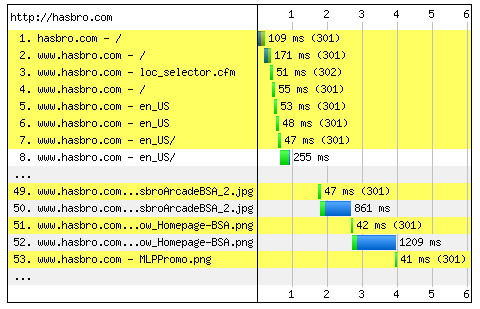
\includegraphics[width=\textwidth]{eliminate_redirects.jpg}
					\caption{Redirects verursachen große Verzögerungen (Abbildung nach webpagtest.org)}
					\label{fig:eliminate_redirects}
				\end{center}
			\end{figure}
			
			Wenn ein Anwender also hs-weingarten.de eingibt erfolgt der DNS Lookup und die TCP Verbindung wird aufgebaut nur um dann zu erfahren, dass die Ressource unter dieser Adresse nicht zur Verfügung steht. Danach erfolgt die DNS auflösung für www.hs-weingarten.de bei dem der gleiche Vorgang vonstatten geht. Es erfolgt die Weiterleitung auf www.hs-weingarten.de/web/willkommen/startseite.html mit wieder dem selben Vorgang.\\

			% TODO: Lösung für dieses URL Mapping Problem?

			Nach 855ms konnte die erste Anfrage an die richtige Zieladresse aufgegeben werden! Ruft man sich die RTT von einem 3G Netz ins Gedächtnis dürfte klar werden, was Weiterleitungen für den Smartphonenutzer bedeuten können. Das der Server rund 3 Sekunden für eine Antwort benötigt ist natürlich noch einmal eine andere Sache.

		\end{itemize}

	% subsection zusammengefasst (end)
	\pagebreak



	\subsection{Kritischer Rendering-Pfad} % (fold)
	\label{sub:critical_render_path}
		Auf Englisch "`critical render path"' genannt, ist der wohl wichtigste Begriff, wenn es um schnelle Ladezeiten geht. Durch die Optimierung des Rendering Pfads kann die benötigte Zeit für das erste Rendern der Seite erheblich verkürzt werden. Das Verständnis des Rendering-Pfads ist zudem eine wesentliche Voraussetzung für die Erstellung von schnellen Webanwendungen und soll in diesem Abschnitt ausführlich erklärt werden. Dabei wird der Begriff in seine zwei Teile Zerlegt: Kritischer und Rendering-Pfad.\\

		Der \texttt{Rendering-Pfad} setzt sich aus den für die Anwendung nötige Ressourcen zusammen. Webanwendungen bestehen schließlich nicht nur aus einer HTML Datei, sondern aus mehreren Javascript und CSS Dateien.

		\begin{figure}[htbp]
			\begin{center}
				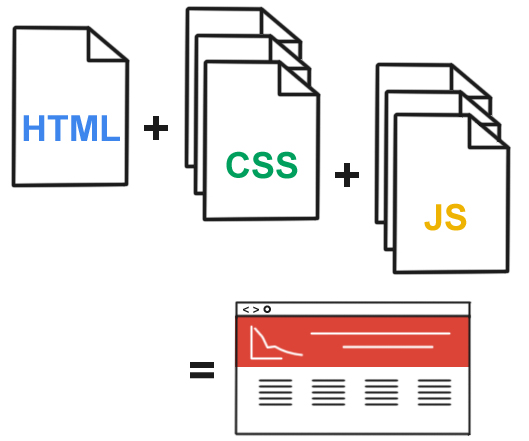
\includegraphics[width=0.4\textwidth]{critical_render_path.jpg}
				\caption{Ressourcen die für das Rendern von nöten sind (Eigene Abbildung)}
				\label{fig:critical_render_path}
			\end{center}
		\end{figure}

		Gegeben ist das folgende Beispiel einer simplen HTML Datei.

		\begin{lstlisting}
			<!DOCTYPE html>
			<meta charset="utf-8">
			<title>Web Performance fuer den mobilen Endanwender</title>

			<link href="assets/styles.css" rel="stylesheet" />
			<script src="assets/script.js"></script>

			<p> Hello world! </p>

		\end{lstlisting}

		Nachdem diese Datei heruntergeladen wurde, beginnt der Browser sie von oben nach unten zu lesen. Dabei stößt er in Zeile 5 auf einen \texttt{link tag} der ihn anweißt diese Datei herunterzuladen. In der nächsten Zeile findet der Browser einen \texttt{script tag}. Auch diese Datei muss herunterladen, interpretiert und ausgeführt werden, denn jede Javascript Datei kann den DOM-Baum oder das CSS manipulieren. Bevor also das "`Hello world"' in Zeile 8 angezeigt werden kann, ist das rendern blockiert. Dieses verhalten nennt sich auch "`Render Blocking"' und wird sowohl von Javascript als auch von CSS Dateien ausgelöst.	Erst dann kann der Browser mit dem rendern beginnen. Dieser Umstand erklärt auch warum die Regel gilt: CSS Dateien in den "`<head>"' und Javascript vor dem schließen des "`</body> tags"' zu platzieren.

		\begin{figure}[htbp]
			\begin{center}
				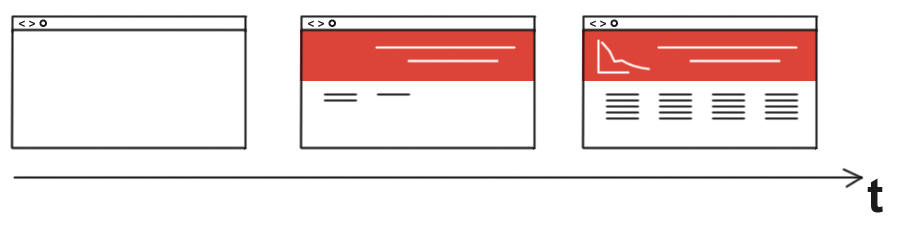
\includegraphics[width=0.75\textwidth]{browser_render.jpg}
				\caption{Der Render Prozess (Eigene Abbildung)}
				\label{fig:browser_render}
			\end{center}
		\end{figure}
	
		\texttt{Critical render path} sind genau die Javascript und CSS Dateien, die für den für das Rendern des \texttt{above the fold} von nöten sind. Um dies umzusetzen ist es nötig, die Ressourcen in 2 Teile zu zerlegen: Für das Rendering absolut notwendig und nicht notwendig. Alle Dateien die nicht notwendig für das erste Rendern sind sollten so lange mit dem Laden verzögert werden, bis die Anwendung geladen ist.

	% subsection critical_render_path (end)


% section die_1000_ms_barriere (end)


\pagebreak

  \section{Entwicklung} % (fold)
\label{sec:entwicklung}
	Dieses Kapitel soll den Entwicklungsprozess konkretisieren und den Optimierungsprozess einer Webanwendung aufzeigen. Es soll erläutern, welche Fragen sich stellten und welche Antworten darauf gefunden wurden. Wie bestimmte Probleme gelöst wurden. Welche Tools und Hilfsmittel zur verwendung kamen. Dies soll ein Bewusstsein dafür schaffen, was möglich ist und wie eine technische Umsetzung aussehen kann. 
	
	\subsection{Tools}
	\label{sub:tools}
		Dies ist eine Auflistung an Tools und nützlichen Seiten, die entweder im Projekt verwendet, oder die für Wertvoll befunden wurden und deshalb hier ihren Platz finden, damit jeder für sich entscheiden kann, ob der Einsatz davon sinnvoll sein könnte.

		\subsubsection{Google Chrome Developer Tool} % (fold)
		\label{ssub:google_chrome_developertool}
			Dieses Tool ist über die Taste F12 im Chrome Browser zu finden. Nützliche Features sind: 

			\begin{itemize}
				\item \texttt{Device Emulation} \footnote{Bei geöffnetem Tool (F12): strg + shift + M oder klick auf das Smartphone Symbol}: Damit lassen sich verschiedene Devices wie Smartphones, Ipad oder verschiedene Desktopauflösungen simulieren. Auch das Touch verhalten wird Simuliert.
				\item In der Device Emulation lässt sich auch die Netzwerkgeschwindigkeit simulieren. Dies ist allerdings nur eine Simulation und kann unter wahren Bedingungen stark abweichen.
				\item Netzwerk: Hier lässt sich das Wasserfallmodell nachvollziehen. Auch lässt sich hier das Caching des Browsers abschalten, wärend das Developer Tool geöffnet ist.
				\item Audits: Unter diesem Reiter bekommt man erste Informationen, welche Verbesserungen es für diese Seite aus dem Gesichtspunkt der Performance ergeben. So wird zum Beispiel aufgezeigt, wie viele CSS Selektoren auf dieser Seite gar keine verwendung finden (gerade bei CSS-Frameworks wie Bootstrap kann es sein, dass rund 90\% der Selektoren keine Verwendung haben)
			\end{itemize}
		% subsubsection google_chrome_developertool (end)

		\subsubsection{Google Pagespeed Insight} % (fold)
		\label{ssub:google_pagespeed_insight}
			Pagespeed Insight ist ein Analysetool für Webanwendungen. Per URL Eingabe wird die Anwendung Aufgerufen und gegen die "`Best Practices"' von Google getestet: \footnote{ \url{http://tinyurl.com/nvxksks} }. Dabei wird ein Rating von 1 (schlecht) bis 100 (gut) vergeben. Mobile und Desktop Version werden voneinander unabhängig bewertet. Findet das Tool verstöße gegen die \texttt{best practices}, so gibt es Hilfestellungen wie zum Beispiel weiterführende Links oder Hinweise zur Behebung des Problems. Für die Verbesserung der Perfomance ist dieses Tool eines der besten Anlaufziele, um einen Überblick zu bekommen wo sich die Probleme befinden. Pagespeed Insight gibt es auch als Plugin für das Google Chrome Developer Tool.\footnote{Plugin - Pagespeed Insight: \url{http://tinyurl.com/mv8fcx8}}
		
		% subsubsection google_pagespeed_insight (end)

		\subsubsection{Google Closure Compiler} % (fold)
		\label{ssub:closure_compiler}
			Ein simples Tool von Google\footnote{\url{http://closure-compiler.appspot.com/}}, mit der Aufgabe Javascript zu verkleinern. Dieser Vorgang nennt sich auch "`minify"' und ist auch für HTML und CSS möglich. Ein Beispiel:

			\begin{lstlisting}[captionpos=t, caption=Input, label=lst:minifyInput]
			/**
			 * urlEncodes an object to send it via post
			 * @param  {Object} object Object with key value pairs
			 * @return {String}        string in format key=value&foo=bar
			 */
			var urlEncode = function (object) {
			  var encodedString = '';
			  for (var prop in object) {
			    if (object.hasOwnProperty(prop)) {
			      if (encodedString.length > 0) {
			          encodedString += '&';
			      }
			      encodedString += encodeURI(prop + '=' + object[prop]);
			    }
			  }
			  return encodedString;
			};
			\end{lstlisting}

			Wird zu:

			\begin{lstlisting}[captionpos=t, caption=Output, label=lst:minifyOutput, breaklines=false]
			var urlEncode=function(c){var a="",b;for(b in c)c.hasOwnProperty(b)&&
			(0<a.length&&(a+="&"),a+=encodeURI(b+"="+c[b]));return a};
			\end{lstlisting}

			Wie zu sehen ist, werden nicht nur alle Kommentare, Leerzeichen und Zeilenumbrüche entfernt, sondern auch Variablennamen werden auf 1 Zeichen reduziert um weitere bytes zu sparen. Die Funktionalität bleibt dabei gewährleistet. Dieser Vorgang ist auch unter dem Namen "`uglify"' bekannt.
		
		% subsubsection closure_compiler (end)

		\subsubsection{Webpagetest} % (fold)
		\label{ssub:webpagetest}
			\url{Webpagetest.org} ist das wohl umfangreichst und beste Website-Analysetool das im Internet zu finden ist. Es ist ein kostenloser Service der hauptsächlich von Patrick Meenan entwickelt wurde. Das Tool ist leicht zu bedienen aber schwer zu beherschen ("`easy to use, hard to master"') und es gibt zahllose Einstellungen und undokumentierte Funktionen auf die man nur in Vorträgen oder Foren stoßt. Es gibt auch ein Buch, dass sich nur mit diesem Tool beschäftigt, beim Verlag \texttt{O'Reilly}.\footnote{Buch - Using WebPagetest: \url{http://shop.oreilly.com/product/0636920033592.do}}.	Die Features für Webpagetest sind vielseitig:

			\begin{itemize}
				\item Es lassen sich Webanwendungen mittels eines in der realität existierenden Geräts testen. So kann vom Standort Dulles VA ein MOTOG zum Testen einer Seite verwendet werden. Dieses Gerät ruft dann auch wirklich die eingegebene URL auf und die darunterliegende Schicht misst die Zeit. Abbildung \ref{fig:wpt-android} zeigt den Teststandort Dulles VA.\footnote{Einen detailierten einblick vom Gründervater und Entwickler Patrick Meenan gibt es hier: \url{http://tinyurl.com/o4b3rxh}}

				\begin{figure}[htbp]
					\begin{center}
						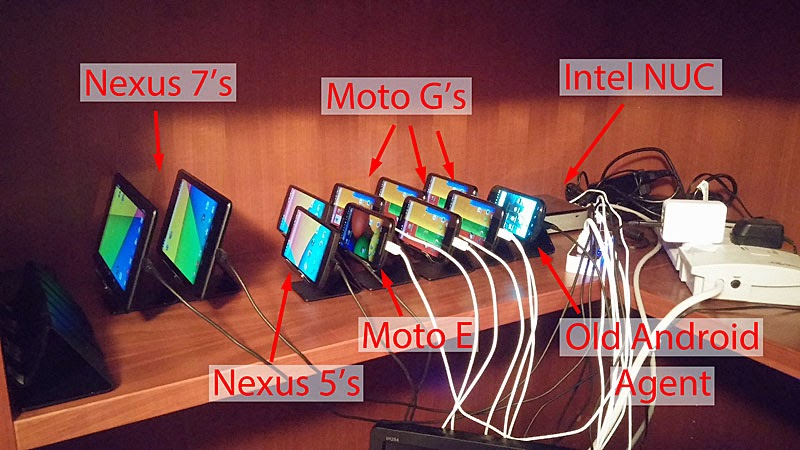
\includegraphics[width=0.5\textwidth]{wpt-android.jpg}
						\caption{Webpagtest Android device farm (Abbildung von \autocite{meenan15})}
						\label{fig:wpt-android}
					\end{center}
				\end{figure}
				\item Webpagetest hat die wohl genauste Erfassung von Netzwerkzeiten und spiegelt damit realitätsgetreu die Ladezeiten einer Seite wieder.

				\item Webpagtest liefer eine enormes Spektrum an Daten und Diagrammen, was ausführliche Analysen zulässt.

				\item Speed Index: Dies ist eine von diesem Tool eigene Maßeinheit zum bestimmen der \texttt{Perceived Performance} einer Seite.

				\begin{quote}
					\textit{"`'The Speed Index metric was added to WebPagetest in April, 2012 and measures how quickly the page contents are visually populated (where lower numbers are better).  It is particularly useful for comparing experiences of pages against each other (before/after optimizing, my site vs competitor, etc) and should be used in combination with the other metrics (load time, start render, etc) to better understand a site's performance."'}\autocite{wegpagetestDocs}
				\end{quote}

				\item Man kann Tests direkt miteinander vergleichen. Das ist möglich, indem diese URL eingegeben wird: \url{www.webpagetest.org/video/compare.php?tests=} und nach dem "`="' Zeichen die Test ID eingibt, beispielsweise "`150310\_8E\_GRH"'.
				Mit einem Komma getrennt wird eine 2. oder 3. ID angefügt. Die Tests werden dann in einer Vergleichsansicht dargestellt.

				\item Filmstrip Ansicht: Damit lässt sich visuell erkennen, wann welches Element gerendet wird.

				\item Video erstellung: Aus der Filmstrip Ansicht lässt sich ein Video erstellen. Das ist vor allem interessant, wenn mit der Vergleichsmethode mehrere Tests geladen sind. Der Ladevorgang der Testläufe wird dann in einem Video Parallel abgespielt. Vor allem für Präsentationen oder vorher / nachher Vergleiche ist dies nützlich.

				\item Test History: Durch eine Registrierung auf der Seite wird ein eigenes Testprofil angelegt in dem alle Test-ID's gespeichert werden.

				\item Testen von verschiedenen Standpunkten: Webpagetest ermöglicht es die eigene Seite von ganz verschiedenen Geographischen Standpunkten aus aufzurufen. Dadurch lässt sich ein Eindruck gewinnen, wie schnell die Seite aus dem Ausland aufrufbar ist und wie stark die Abweichung sein kann.

				\item API: Webpagtest hat eine offene API (Schnittstelle) durch die das Tool von außerhalb erreichbar ist. So lässt sich ein Test beispielsweise in Google-Spreadsheets aufrufen und das Ergebnis direkt in eine Tabelle schreiben. Mehr dazu in Punkt: \ref{..} ?. Diese Schnittstelle Limitiert allerdings die Anzahl an Tests pro Tag auf 200. Für mehr muss man sich eine eigene Private Instanz erstellen. 
				%todo ref

				\item Private Instanz: Da webpagetest Open Source ist, gibt es die möglichkeit eine eigene Private Instanz aufzusetzen. Dies kann sowohl per Amazon Cloud oder auf einem eigenen Server geschehen. Damit lassen sich dann soviele Tests ausführen, wie die Leistungs des Servers bietet.

			\end{itemize}
		% subsubsection webpagetest (end)	

		\subsubsection{Pingdom} % (fold)
		\label{ssub:pingdom}
			\url{http://tools.pingdom.com/fpt/} ist eine Alternative zu Webpagetest. Auch damit lässt sich eine URL nach Performanceproblemen analyisieren. Die Ergebnisse sind nicht so genau wie mit Webpagetest und auch ein Testen mit Smartphones fehlt. Bei einer kostenlosen Anmeldung erhält man allerdings ein System zur Überwachung der eigenen Webanwendung. Bei Ausfall oder zu hoher Last kann eine SMS versendet werden um den Admin auf diesen Umstand hinzuweisen. Durch einbetten eines Scripts auf der eigenen Seite lässt sich die Response zeit aufzeichnen (siehe Abbildung \ref{fig:choose_a_good_host}). Dieses tracking nennt man auch "`real user monitoring"' und ist zum Beispiel auch durch Google Analytics in solch einer Form abrufbar.

		
		% subsubsection pingdom (end)

		\subsubsection{Speedcurve} % (fold)
		\label{ssub:speedcurve}
			Ist ein kommerzielles Tool basierend auf Webpagetest. Es liefert einen "`life monitoring"' Service mit dem sich Webanwendungen vergleichen lassen. So kann man zum Beispiel die eigene Webanwendung dauerhaft und über einen längeren Zeitraum mit denen der Konkurenz vergleichen. 

			\begin{figure}[htbp]
				\begin{center}
					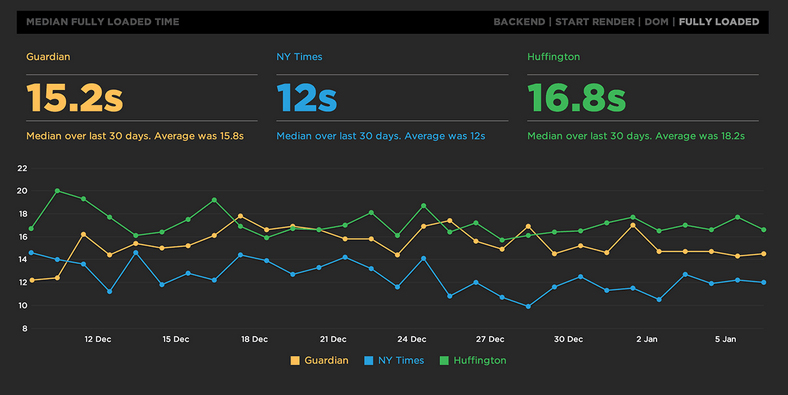
\includegraphics[width=0.7\textwidth]{speedcurve.jpg}
					\caption{Speedcurve Life Monitoring (Abbildung von \url{http://speedcurve.com/})}
					\label{fig:speedcurve}
				\end{center}
			\end{figure}

		% subsubsection speedcurve (end)

		\subsubsection{Google Spreadsheet} % (fold)
		\label{ssub:google_spreadsheet}
			Ist im Grunde wie Microsofts Excel. In Tabellen können Werte eingetragen und Berechnungen ausgeführt werden.
			Der große Vorteil an Google Spreadhseet besteht in der Möglichkeit, dass es einen Skript Editor gibt, mit dem sich kleine Programme schreiben lassen. So sind zum Beispiel API Abfragen möglich, dessen Ergebnis dann direkt in die Tabelle geschrieben werden kann.		
		% subsubsection google_spreadsheet (end)

		\subsubsection{Feed the Bot} % (fold)
		\label{ssub:feed_the_bot}
			\url{http://www.feedthebot.com/pagespeed/} bietet umfassende Artikel zu SEO und web performance. Wenn man sich mit dem Thema web performance beschäftigen möchte, ist dies eine erstklassige Anlaufstelle.
		% subsubsection feed_the_bot (end)


		\subsubsection{What Does My Site Cost?} % (fold)
		\label{ssub:what_does_my_site_cost}
			"`Was kostet es eigentlich meinene Seitenbesucher, wenn sein Datenvolumen für diesen Monat aufgebraucht ist und er pro verbrauchtes MB zur Kasse gebeten wird?"' Diese Frage versucht diese Webanwendung zu klären und visuell darzustellen.\\
			\url{http://whatdoesmysitecost.com/} benutzt die webpagetest Schnittstelle um eine eingegebene URL zu Analyisieren und berechnet aus den billigsten Anbieteren pro Land einen Preis für den Aufruf der Seite mittels Smartphone:

			\begin{quote}
				\textit{"`Prices were collected from the operator with the largest marketshare in the country and the for the least expensive plan with a (minimum) data allowance of 500 MB over (a minimum of) 30 days. Prices include taxes. Because these numbers are based on the least expensive plan, they are \textbf{best case} scenarios."'}\autocite{siteCosts}
			\end{quote}

		\begin{figure}[htbp]
			\begin{center}
				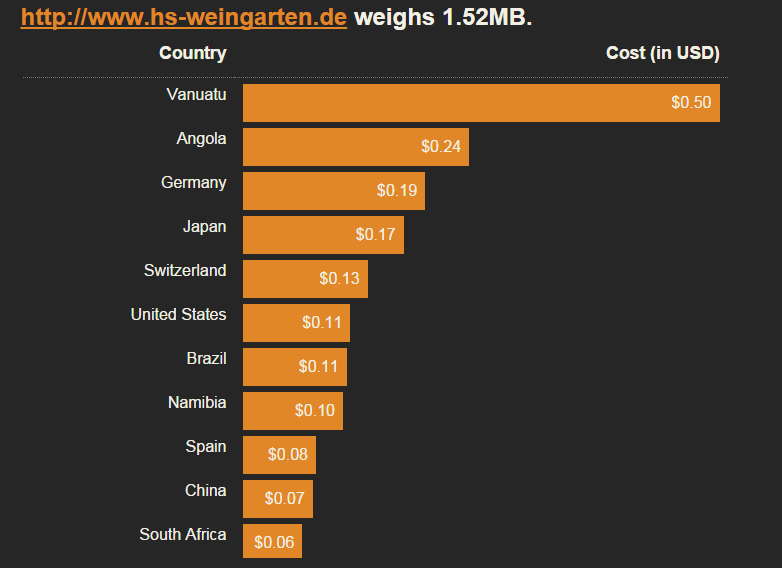
\includegraphics[width=0.7\textwidth]{what_does_my_site_cost.jpg}
				\caption{Find out how much it costs for someone to use your site on mobile networks around the world.\autocite{siteCosts}}
				\label{fig:what_does_my_site_cost}
			\end{center}
		\end{figure}

		In Deutschland kostet also der Seitenaufruf von hs-weingarten.de rund 20 Cent. Dieses Tool stellt auf sehr schöne Art und Weise dar, dass schlechte web performance nicht nur den Anwender verägert, sondern zusätzlich zum Ärger auch noch bares Geld kosten kann.
		% subsubsection what_does_my_site_cost (end)

		\subsubsection{Critical Path CSS Generator} % (fold)
		\label{ssub:critical_path_css_generator}
			Im Kapitel "`Brechen der 1000 ms Barriere"'\ref{sec:die_1000_ms_barriere} wurde gesagt, man solle das CSS des above the folds direkt in das HTML als \texttt{inline CSS} schreiben. \url{http://jonassebastianohlsson.com/criticalpathcssgenerator/} erstellt aus einer gegebener URL und dem dazugehörigen CSS genau den CSS-Code, der für den above the fold Bereich nötig ist. Das Ergebnis lässt sich dann bequem in das eigene HTML einfügen.\\

			Dieser Generator funktioniert allerdings nur dann gut, wenn sowohl die Smartphone, als auch Desktop Darstellung identisches CSS haben. Bootstrap zum Beispiel manipuliert die Navigation auf der Smartphone Ansicht per Javascript und fügt dabei Elemente ein. Diese Elemente kennt dieser Generator natürlich nicht und kann sie folglich auch nicht beachten. Eine alternative Methode wird in Kapitel ... \ref{..} ? vorgestellt.

		% subsubsection critical_path_css_generator (end)

		\subsubsection{Http Archive} % (fold)
		\label{ssub:http_archive_bigqueri_es}
			\url{http://httparchive.org/} ist ein Archiv der populärsten Seiten des Internets und bietet eine Vielzahl an statistischen Auswertungen, Trends und Daten.
			\begin{quote}
				\textit{"`[HTTP Archive] is a permanent repository of web performance information such as size of pages, failed requests, and technologies utilized. This performance information allows us to see trends in how the Web is built and provides a common data set from which to conduct web performance research."' \autocite{httpArchive}}
			\end{quote}
			
		% subsubsection http_archive_bigqueri_es (end)

		\subsubsection{Perf Tooling Today} % (fold)
		\label{ssub:perf_tooling_today}
			\url{http://perf-tooling.today/} ist wohl die Umfassendste Sammlung an web performance Tools und Material im Internet. Es hat eine Liste von 105 Tools, 51 Artikel, 27 Videos und 14 Slidedecks (Stand: 12.03.15).
		
		% subsubsection perf_tooling_today (end)

		\subsubsection{Twitter} % (fold)
		\label{ssub:twitter}
			Twitter bietet die Möglichkeit am Puls der Zeit zu sein und unter dem Hashtag \#webperf und \#perfmatters erhält man neuste Erkentnisse, Tools oder Links, die sonst unentdeckt bleiben.
		
		% subsubsection twitter (end)
	\pagebreak
	% subsection tools (end)


	\subsection{Ausgangspunkt}
	\label{sub:ausgangspunkt}
		Im folgenden Abschnitt soll der Prozess beschrieben werden, um von einer langsamen Webanwendung zu einer schnellen zu gelangen. Von Beginn an war es wichtig, den Verbesserungsablauf zu Dokumentieren und in konkrete Daten zu fassen. Wie bereits unter Punkt \ref{ssub:google_spreadsheet} beschrieben, bietet Google Spreadsheets die möglichkeit Skripte zu schreiben und die Ergebnisse direkt in eine Tabelle auszugeben. Diesen Umstand hat sich \texttt{Andy Davies} zu nutzen gemacht und ein Programm\footnote{WebPageTest Bulk Tester via GitHub: \url{https://github.com/andydavies/WPT-Bulk-Tester}} geschrieben (MIT License), dass es ermöglicht Webpagtestest innerhalb einer Google Tabelle\footnote{Das Google Dokument ist hier zu finden: \url{http://tinyurl.com/nv4pge5}} aufzurufen. Damit wurde während der Entwicklungsphase täglich tests aufgezeichnet.\footnote{Die gesamten Daten sind hier zu finden: \url{http://tinyurl.com/l5usz79}} Die Auswertung dieser Daten erfolgt in Punkt \ref{..} ?\\
		%todo ref

		Da nur in Dulles VA eine Testinstanz mit richtigen Smartphones zur Verfügung steht, wurde mittels der \texttt{Microsoft Azure Cloud} die selbe Seite auch in den USA gehostet, um die Latenz zwischen USA und Europa zu eliminieren. Dadurch lässt sich exakter bestimmen, wie schnell ein Smartphone mit 3G Netz die Seite aufrufen kann. Leider steht keine Testinstanz mit 4G Netz zur Verfügung.\\

		Als Ausgangspunkt dient die Seite \url{http://andreaslorer.de/old/}. Zu beginn des Optimierungsprozesses gab es folgenden Ausgangspunkt (Daten via Developer Tool \& webpagetest):\\

		Desktop: \footnote{Webpagtest: \url{http://www.webpagetest.org/result/150312_Z1_18QD/}}
		\begin{itemize}
			\item 42 requests: 30 Images, 5 JS, 3 CSS, 4 other
			\item 1000 kb Seitengröße
			\item Speed Index: \textbf{3584}
			\item Start Render: \textbf{1399}  ms
			\item Load Time: 1926 ms
			\item TTFB: 690 ms
		\end{itemize}

		Mobile: \footnote{Webpagtest: \url{http://www.webpagetest.org/result/150308_A1_2W4/}}
		\begin{itemize}
			\item 17 requests: 4 Images, 5 JS, 3 CSS, 4 other
			\item 363 kb Seitengröße
			\item Speed Index: \textbf{10642}
			\item Start Render \textbf{6968} ms
			\item Load Time: 5587 ms
			\item TTFB: 1292 ms
		\end{itemize}

		Diese Werte sind nicht gut und für dieses Projekt wurden eine Start Render Zeit von weniger als einer Sekunde und ein Speed Index von unter 1000, für sowohl Mobile- als auch Desktopgeräte, angestrebt.\\

		Der erste Schritt war es, die Seitengröße zu verringern. Aus diesem Grund wurde das Framework gewechselt und die Seite neu Aufgebaut. Bootstrap ist zwar ein sehr populäres Framework, hat aber gerade für kleine Seiten sehr viele Komponenten, die keine Verwendung finden (oft auch als Overhead bezeichnet). Bootstrap lässt sich zwar per "`Customize"' Funktion so zusammenstellen, dass nur die Komponenten zur Verfügung gestellt werden, die für das eigene Projekt von Nöten sind, es ist aber dennoch ein Framework mit relativ großem Volumen (~30 bis 90 kb). Die Alternativen zu Bootstrap sind vielzählig. Die Entscheidung für dieses Projekt fiel auf \url{http://purecss.io/}. Dieses Framework von Yahoo ist Komprimiert gerade einmal \textbf{4 kb} groß, vollkommen responsive und kommt mit den wichtigsten Komponenten wie einer Navigations Bar, Buttons, Tabellen, Menüs und Form Elementen. Je nach gewählten Komponenten, benötigt es kein Javascript und kein JQuery. Dadurch lassen sich weitere Kilobytes als auch Requests einsparen.\\
		Da Bootstrap seine eigene Icon-Font liefert, musste hier eine Alternative gefunden werden. "`Font Awesome"'\footnote{Font-Awesome: \url{http://fortawesome.github.io/Font-Awesome/}} bietet dabei eine der umfangreichsten Icon Sammlungen im Web an und ist unter der \texttt{Open Font License} komplett frei benutzbar (auch kommerziell). Font Awesome ist mit seinen 519 Icons allerdings nicht gerade ein Leichtgewicht und kann bis zu 100 kb groß sein. Da auf der Seite \url{http://andreaslorer.de} weniger als 20 Icons zum Einsatz kommen ist der Überschuss folglich enorm. Deshalb gibt es eine Webanwendung namens \url{http://fontello.com}. Damit lassen sich aus einer Vielzahl an Icons genau die wählen, die für die eigene Seite benötigt werden. Auch das Wählen aus verschiedenen Icon-Sammlungen ist möglich. Heruntergeladen wird anschließend eine ZIP-Datei. Das Resultat: Die neue Version der Seite benötigt nur noch 5.6 kb für die Icons. Verglichen mit: Bootstrap 43 kb, Font-Awesome 97 kb.\\

		Als nächstes wird die Webanwendung mittels \texttt{Pagespeed Insight}\ref{ssub:google_pagespeed_insight} Analyisert. Das Ergebnis liefert Anhaltspunkte, was für schnellere Ladezeit alles umgesetzt werden sollte. Im folgenden soll erläutert werden, was es alles an Verbesserungen gibt und wie eine mögliche Umsetzung in der Praxis aussieht.

		% zusammenfügen mit best practices?

		\subsubsection{Render Blocking Javascript} % (fold)
		\label{ssub:render_blocking_javascript}
			Bereits unter Punkt \ref{ssub:rendering_pfad} ist das Blockierende Verhalten von Javascript und CSS angesprochen worden. Grundvoraussetzung für diesen Punkt ist, dass das Javascript der Webanwendung in ihre, für das Rendern kritische und für das Rendern unkritische Teile zerlegt wurde. 

			Der Browser stellt bereits von Haus aus zwei Attribute bereit, mit denen sich Skripte asynchron herunterladen lassen. Diese Attribute heißen "`async"' und "`defer"' und werden von jedem Browsertyp unterstützt.\autocite{canIuse} Sie erlauben es, dass der Browser nicht auf das Herunterladen der Dateien warten muss, sondern mit dem Parsen des Dokuments fortfahren darf. Async wird direkt nach dem herunterladen ausgeführt und dafür muss das Parsen pausiert werden. Defer hingegen unterscheidet sich von async in zwei Punkten: 1. Das Skripte wird nach Ende des Parsens ausgeführt. 2. Mit defer verzögert geladene Skripte werden in genau der Reihenfolge ausgeführt, wie die Reihenfolge der Skripte im HTML Dokuments vorliegen.
			
			\begin{figure}[htbp]
				\begin{center}
					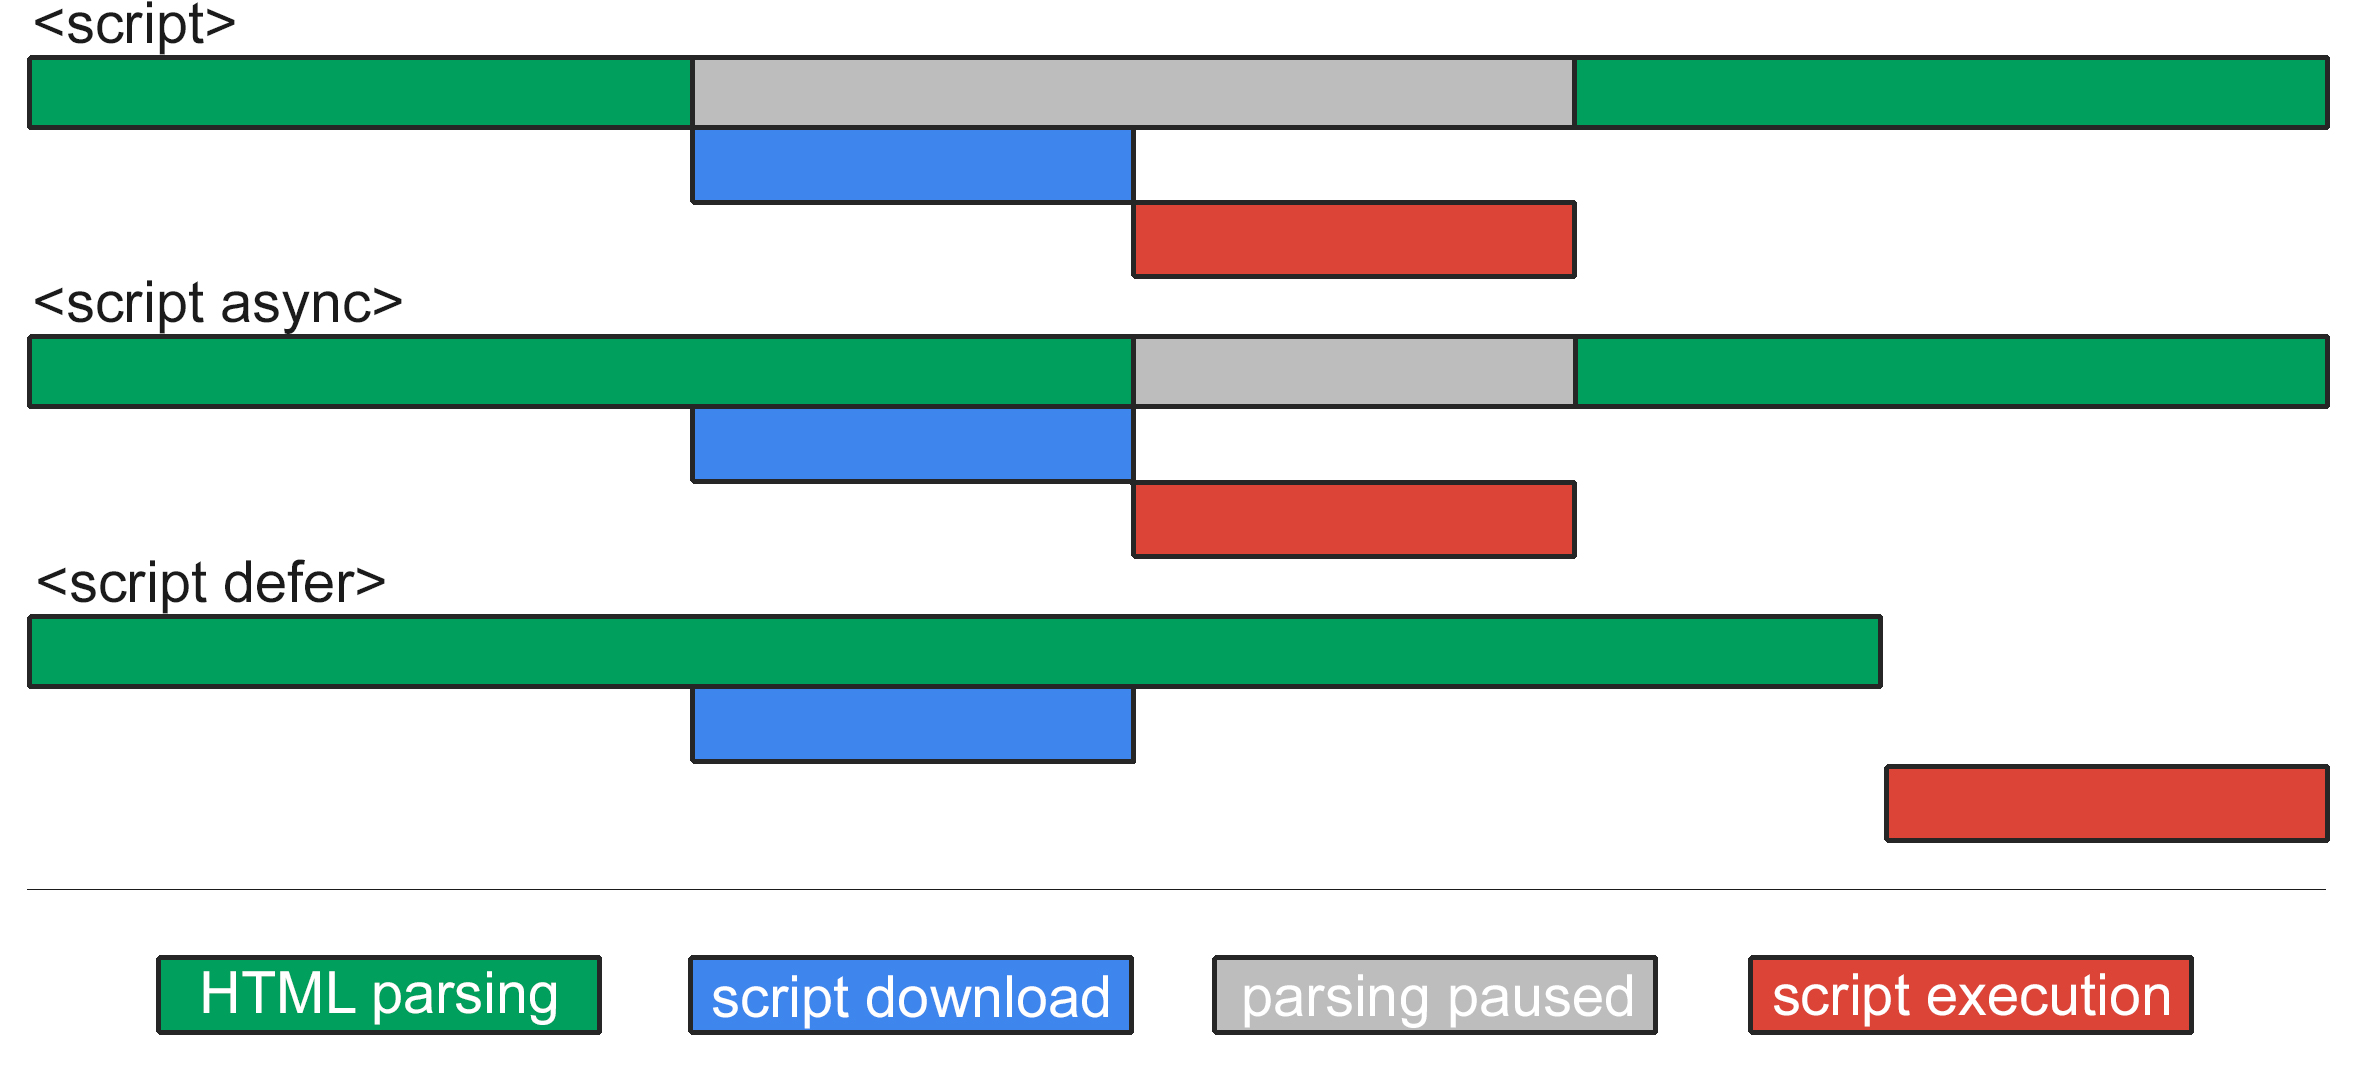
\includegraphics[width=\textwidth]{defer_scripts.jpg}
					\caption{Script-Tags mit verschiedenen Attributen (Abbildung nach \autocite{growing})}
					\label{fig:defer_scripts}
				\end{center}
			\end{figure}

			Diese Methode erlaubt es, Skripte parallel herunterzuladen, ohne dass der Renderprozess warten muss. Was damit nicht erreicht werden kann ist, dass der Download so lange verzögert wird, bis die für die Seiten primär wichtigen Ressourcen zuerst heruntergeladen wurden.\\

			Mit Hilfe des Javascripts in Listing \ref{lst:deferJs}, kann die Datei "`defer.js"' komplett mit dem Laden verzögert werden, bis der Ladeprozess der Seite abgeschlossen ist.\\
	
			\begin{lstlisting}[captionpos=b, caption=Javascript nach \autocite{deferJS}, label=lst:deferJs]
			// the function to asynchronous load js
			function loadJS( src, cb ){
				"use strict";
				var ref = window.document.getElementsByTagName( "script" )[ 0 ];
				var script = window.document.createElement( "script" );
				script.src = src;
				script.async = true;
				ref.parentNode.insertBefore( script, ref );
				if (cb && typeof(cb) === "function") {
					script.onload = cb;
				}
				return script;
			}

			// the function call to load your script
			loadJS( "path/to/script.js" );
			\end{lstlisting}

			Dieses Skript hat einen Nachteil: Es kann nicht mehrere Skripte laden, die voneinander Abhängen und deren Reihenfolge wichtig ist, um die Funktionalität zu gewährleisten. 

			\begin{quote}
				\textit{"`loadJS does nothing to manage execution order of requested scripts, so we do not advise using it to load multiple javascript files that depend on one another. It simply fetches a script and executes it as soon as possible. You can certainly use loadJS to load multiple scripts as long as those scripts are designed to execute independently of any other scripts being loaded by loadJS."'\autocite{deferJS}}
			\end{quote}

			So gibt es Skripte (Skript A) die von anderen Frameworks wie zum Beispiel JQuery (Skript B) abhängen. Das bedeutet, wenn Skript A schneller heruntergeladen und ausgeführt wird als Skript B, A bereits Funktionen von B aufruft, die noch nicht zur Verfügung stehen. Daraus resultiert ein Fehlschlagen des Skripts und somit können teile der Webanwendung nicht mehr wie beabsichtigt Funktionieren.\\

			Darum gibt es Skripte die genau diese Funktionalität bereitstellen können. Skript A und B werden gleichzeitig heruntergeladen, A wird aber erst genau dann Ausgeführt, wenn B zur Verfügung steht.\\

			\url{http://headjs.com/} kann das erreichen. Durch das Herunterladen und Einfügen in das HTML Dokument, kann per Funktionsaufruf die Abhängigkeit festgelegt werden:

			\begin{lstlisting}[captionpos=b, caption=Headjs dependency loading (Listing nach http://headjs.com/), label=lst:headjs]
				// Load up some script A and then script B
				head.load("jQuery.js", function() {
				    // Call a function when done
				    console.log("Done loading jQuery");
				    head.load('defer.js')
				});
			\end{lstlisting}

			Headjs hat den Nachteil, dass es auch noch andere Funktionalitäten außer dem Laden von Javascript ermöglicht. Dies wird aber nicht benötigt und deshalb ist Headjs mit 2.1 kb doch zu groß, um es \texttt{Inline} in das HTML Dokument zu schreiben. Eine bessere Alternative ist \texttt{jQl}. \footnote{jQl an asynchronous jQuery Loader: \url{http://www.yterium.net/jQl-an-asynchronous-jQuery-Loader}}
			Die Verwendung ist sehr Simpel:

			\begin{lstlisting}[captionpos=b, caption=jQl asynchronous jQuery-Loader, label=lst:jQl]
				<script type="text/javascript">
					// first include jQl inline (missing here) then call these functions
				  jQl.loadjQ('jquery.js');
				  jQl.loadjQdep('defer.js');
				</script>
			\end{lstlisting}

			Dieses Skript sagt im Grunde: Lade beide Dateien gleichzeitig herunter, beachte aber die Abhängigkeit (loadjQdep steht für: load dependency) von defer.js gegenüber JQuery. Ist defer.js früher heruntergeladen als JQuery, so wird gewartet und anschließend werden die Skripte in der richtigen Reihenfolge ausgeführt.\\

			Für die Webseite \url{http://andreaslorer.de} wurde sowohl defer, als auch das Skript \texttt{jQl} verwendet. "`<script defer src='critical.js'></script>"' wird dabei in den "`<head>"' bereich des HTML Dokments platziert, damit es möglichst früh erkannt wird und der Download bereits beginnen kann und das Skript aus Listing \ref{lst:jQl} befindet sich vor dem "`</body>"'-Tag.

			\pagebreak

		% subsubsection render_blocking_javascript (end)

		\subsubsection{Render Blocking CSS} % (fold)
		\label{ssub:render_blocking_css}
			Wie Javascript blockiert auch CSS das Rendern der Seite. In Listing \ref{deferCSS} ist ein Skript der Filament Group uzu sehen. Dieses Skript ermöglicht es CSS Verzögert zu laden. 

			\begin{lstlisting}[captionpos=b, caption=load a CSS file asynchronously, label=lst:deferCSS, breaklines=false]
			<script>
				// minified script after: 
				// https://github.com/filamentgroup/loadCSS/blob/master/loadCSS.js
				// [c]2014 @scottjehl, Filament Group, Inc.
				// Licensed MIT
	 			function loadCSS(e,a,g,h){function f(){for(var a,c=0;c<d.length;c++)d[c].href&&
	 				-1<d[c].href.indexOf(e)&&(a=!0);a?b.media=g||"all":setTimeout(f)}
	 				var b=window.document.createElement("link");a=a||
	 				window.document.getElementsByTagName("script")[0];
	 				var d=window.document.styleSheets;b.rel="stylesheet";b.href=e;b.media="only x";
	 				b.onload=h||function(){};a.parentNode.insertBefore(b,a);f();return b
	 			};

	  		loadCSS( "path/to/css" );
			</script>

			<!-- fallback if javascript is disabled in browser -->
			<noscript><link href="path/to/css"></noscript>
			\end{lstlisting}

			Mehr als dieses Skript ist nicht notwendig.
				
		% subsubsection render_blocking_css (end)

		\subsubsection{Inline von CSS} % (fold)
		\label{ssub:inline_von_css}
			Kleinere Mengen an CSS lassen sich direkt \texttt{Inline} in das HTML Dokument einfügen. Dadurch sind diese gleich mit dem ersten Request bereits im Dokument enthalten und müssen nicht erst angefordert und heruntergeladen werden.
		% subsubsection inline_von_css (end)

		\subsubsection{Ressourcen reduzieren} % (fold)
		\label{ssub:ressourcen_reduzieren}
			Das schnellste Byte ist das, dass nicht gesendet wird und der schnellste Request ist der, der nicht gestellt wird. Deshalb gibt es drei Maßnahmen die für eine Webanwendung umgesetzt werden sollte:

			\begin{itemize}
				\item "`Minify"': Kommentare, Leerzeichen oder Zeilenumbrüche sind für die Funktionalität nicht notwendig. Bei der Verkleinerung des HTML- CSS oder Javascript Codes werden diese entfern und dadurch die Dateigröße verkleinert. Wie unter Punkt \ref{ssub:google_pagespeed_insight} angesprochen, gibt es Pagespeed Insight auch als Chrome-Erweiterung. Damit ist es möglich, eine reduzierte Version des HTML Dokuments zu erzeugen. Für Javascript ist der Closure Compiler (\ref{ssub:closure_compiler}) das richtige Werkzeug. CSS lässt sich per \url{http://cssminifier.com/} verkleinern.
				\item "`Uglify"': Dabei werden Variablennamen, auf nur wenige Zeichen reduziert. Aber auch Code wird teilweise umgeschrieben, wenn für einen verwendeten Ausdruck beispielsweise eine kürzere Schreibweise existiert.

				\begin{lstlisting}[captionpos=b, caption=Beispiel: Uglify eines Ausdrucks, label=lst:uglify]
				// input:
				if(foo){
					bar();
				}
				else{
					boo();
				}

				// output:
				foo?bar():boo();
				\end{lstlisting}

				Input und Output sind identisch in ihrem Ausdruck, die Zeichenanzahl wurde aber von 27 auf 16 verringert.

				\item "`Concatenate"': Damit ist das Zusammenfügen von einzelnen Dateien zu einer Einzigen gemeint. Dadurch lassen sich zusätzliche Requests einsparen. Dies hat den Vorteil, dass sowohl der TCP Slow start nur einmal eintritt als auch nur eine TCP Verbindung aufgebaut werden muss. Zusätzlich werden weniger TCP Verbindungen belegt, denn dafür gibt es, wie bereits erwähnt wurde (Punkt \ref{sub:http_1_1}), ein Limit.
			\end{itemize}
		% subsubsection ressourcen_reduzieren (end)

		\subsubsection{CSS-Bereitstellung optimieren} % (fold)
		\label{ssub:css_bereitstellung_optimieren}
			Wenn externe Ressourcen klein sind, können diese direkt in das HTML Dokument \texttt{Inline} platziert werden. Dabei sollte darauf geachtet werden, dass das HTML Dokument Komprimiert nicht die 14 kb Marke überschreitet. Dadurch kann es im ersten round trip geliefern werden. CSS Dateien die groß sind sollten per \texttt{Link-Tag} eingebunden werden und mittels Skript Verzögert geladen werden. Das CSS für den above the fold Bereich sollte \texttt{Inline} im "`<head>"' Bereich der Seite stehen. 
		% subsubsection css_bereitstellung_optimieren (end)

		\subsubsection{Antwortzeit des Servers reduzieren} % (fold)
		\label{ssub:antwortzeit_des_servers_reduzieren}
			Die Zeit zur Antwort des Servers lässt sich zum Beispiel mit Webpagtest herausfinden. Ein Server sollte auf eine Response Zeit von unter 200 ms kommen. \textit{"`Es gibt Dutzende potenzielle Faktoren, die die Antwortzeit Ihres Servers beeinträchtigen können: eine langsame Anwendungslogik, langsame Datenbankabfragen, langsames Routing, Frameworks, Bibliotheken, CPU-Ressourcenmangel oder Speicherplatzmangel. Berücksichtigen Sie zur Verkürzung der Antwortzeit Ihres Servers alle diese Faktoren."'} \autocite{google15}. Bereits unter Punkt: \ref{sub:zusammengefasst} wurde es nahegelegt ein gutes Hosting zu wählen. Besser Sie wechseln ihr Hosting als ihre Kunden den Service.
		% subsubsection antwortzeit_des_servers_reduzieren (end)

		\subsubsection{Browser-Caching nutzen} % (fold)
		\label{ssub:browser_caching_nutzen}
			Fehlendes Browser-Caching (das lokale Speichern von Daten) wird von Pagspeed Insight bemängelt, wenn der Server bei seiner Antwort keinen expliziten \texttt{Caching-Header} versendet.
			Durch das Speichern von statischen Ressourcen wie Javascript, Stylesheets und Bildern kann Zeit eingespart werden, wenn der Besucher die Webanwendung ein weiteres mal aufruft. Generell sollten alle statischen Ressourchen außer das HTML Dokument selbst, gechached werden.\\

			Um auf dem Server (Apache) das Caching von statischen Ressourcen zu ermöglichen, ist ein Eintrag in die \texttt{.htaccess} Datei des Servers nötig. Folgender Eintrag sollte dort platziert werden:

		  \begin{lstlisting}[captionpos=b, caption=Aktivieren von Browser Caching in Apache (Listing nach: \autocite{sextonCaching}), label=lst:caching, language=bash]
		  	## EXPIRES CACHING ##
		  	<IfModule mod_expires.c>
		  	ExpiresActive On
		  	ExpiresByType image/jpg "access 1 year"
		  	ExpiresByType image/jpeg "access 1 year"
		  	ExpiresByType image/gif "access 1 year"
		  	ExpiresByType image/png "access 1 year"
		  	ExpiresByType text/css "access 1 year"
		  	ExpiresByType text/woff "access 1 year"
		  	ExpiresByType application/pdf "access 1 year"
		  	ExpiresByType text/x-javascript "access 1 year"
		  	ExpiresByType application/x-shockwave-flash "access 1 year"
		  	ExpiresByType image/x-icon "access 1 year"
		  	ExpiresDefault "access 1 month"
		  	</IfModule>
		  	\#\# EXPIRES CACHING \#\#
		  \end{lstlisting}

		  Listing \ref{lst:caching} hat 2 Aufgaben. Erstens: Es setzt die Ablaufzeit für alle statischen Ressourcen auf 1 Jahr und erfüllt damit den von Google empfohlenen Wert. Längere Speicherzeiten sind dagegen nicht Empfohlen, da dies gegen die RFC-Richtlinien verstoßen würde \autocite{google14Caching}. Zweitens: Es wird mit dem HTTP Request ein Header mit gesendet. Dieser ermöglicht es dem Browser seine lokal gespeicherten Ressourcen zu managen. Er besteht aus folgenden Teilen und es ist jeweils nur \textbf{eine} der Optionen nötig.

		  \begin{itemize}
		  	\item Last-Modified: date
		  	\item ETag: ID
		  \end{itemize}

		  Diese beiden Header ermöglichen es dem Browser zu überprüfen, ob sich die gecachten Ressourcen geändert haben oder noch identisch sind. Last-Modified ist dabei das Datum der letzten Änderung und der ETag-Header ist ein automatisch generierter Wert, der die Datei eindeutig Identifiziert.\\
		  Beim erneuten Laden einer Seite werden diese Header zurück an den Server gesendet und verglichen. Wenn die Datei auf dem Server geändert wurde stimmen die Werte nicht überein und der Server schickt eine entsprechende Antwort zurück.

		  \begin{itemize}
		  	\item Cache-Control: max-age=value
		  	\item Expires: date
		  \end{itemize}

		  Mit diesen Headern ist es möglich Serveranfragen komplett zu vermeiden. "`Sämtliche vom Browser ausgegebenen HTTP-Anfragen werden zuerst an den Browsercache weitergeleitet, um zu überprüfen, ob eine gültige Antwort im Cachespeicher vorliegt, die der Anfrage entspricht. Liegt eine Übereinstimmung vor, wird die Antwort aus dem Cache ausgelesen, wodurch sowohl die Netzwerklatenz als auch die durch die Übertragung anfallenden Datenkosten umgangen werden."'\autocite{grigorikCaching} Das bedeutet, dass die Latenz bei Smartphones für gecachte Dateien komplett negiert werden kann. Gültige Ressourcen werden erst gar nicht angefragt, sondern gleich aus dem Cache geladen. Ungültige oder abgelaufene Ressourcen werden dagegen vom Server geholt. Ohne diesen Header, muss der Browser für jede in seinem Cache befindliche Ressource, den Server anfragen. Dafür sind jedes mal ein round trip nötig.\\

		  \begin{figure}[htbp]
		  	\begin{center}
		  		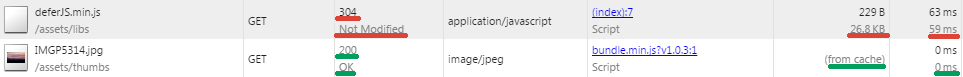
\includegraphics[width=\textwidth]{caching_enabled.jpg}
		  		\caption{Gecachte Ressourcen müssen nicht mehr abgefragt werden}
		  		\label{fig:caching_enabled}
		  	\end{center}
		  \end{figure}
		  
		  Das rot unterstrichene zeigt, dass 59 ms im Netzwerk verbraucht wurde (Kabel Verbindung). Der Server antwortete mit: "`Not-Modified"'. Grün zeigt, dass keinerlei Kommunikation mit dem Server nötig ist sondern die Datei, in diesem Fall ein Bild, direkt aus dem Cache geholt wird.\\
		  Fazit: Ohne Cache-Control lässt sich durch die Browser eigene Caching Funktionalität das erneute Herunterladen der Datei vermeiden. Mit Cache-Control kann sowohl das Herunterladen als auch der gesamte Verbindungsaufbau zum Server vermieden werden.\\
		 
		  Was aber wenn sich zum Beispiel eine CSS-Datei geändert hat? Dann würden nun Besucher mit leerem Cache eine andere Darstellung erhalten, wie Besucher mit der gecachten Version. Dafür gibt es mehrere Lösungsansätze.

		  \begin{enumerate}
		  	\item Die HTML Datei sollte nicht gecached werden da sonst Änderungen nicht mehr den Anwender können.
		  	\item Eine für die Datei angemessene max-age: Dateien die sich oft ändern dürfen auch entsprechend niedrige max-age Werte haben. Dadurch wird die Datei Zeitnah für alle Anwender neu Angefordert.
		  	\item Ressourcen können mit einer ID versehen werden: \texttt{styles.css} wird in \texttt{styles.v1.0.1.css} umbenannt.
		  	\item Alternativ zur ID ist auch in \texttt{Fingerprint} möglich. Dabei wird eine ID aus der Datei generiert. Ändert sich die Datei so ändert sich auch der Fingerprint. Dieser Fingerprint wird auch wiederrum dem Dateiname angefügt. Das kann so aussehen: \texttt{styles.82s0dfsa.css}.\footnote{Dieses Verfahren lässt sich auch automatisieren, ich verweise auf folgenden Artikel: \url{https://adactio.com/journal/8504}}
		  \end{enumerate}

		  Browser-Caching ist eine mächtige Funktionalität die sich jeder zu nutzen machen sollte. Sie ist zudem ganz einfach mit nur einem Eintrag in die \texttt{.htaccess}-Datei realisierbar. Allerdings hat eine Studie von Yahoo ergeben, dass 40-60\% der Besucher beim Seitenaufruf einen leeren Cache haben und rund 20\% aller aufgerufenen Seiten wurden mit einem leeren Cache aufgerufen.
			\begin{quote}
				\textit{"`[...] I don't know about you, but these results came to us as a big surprise. It says that even if your assets are optimized for maximum caching, there are a significant number of users that will always have an empty cache."'\autocite{yahoo07}}
			\end{quote}

			Folglich macht es Sinn, die Geschwindigkeit der Seite für die sogenannten "`first users"' zu optimieren und nicht von einem gecachten Zustand der Seite auszugehen.\\
			\texttt{Feed-The-Bot} stellt ein Tool\footnote{Tool: \url{http://www.feedthebot.com/tools/if-modified/}} zu Verfügung, mit dessen Hilfe sich überprüfen lässt, ob die eigene Webseite "`Browser-Caching"' richtig einsetzt. Abbildung Nummer \ref{fig:expires_header} zeigt Links eine Seite mit aktiviertem Browser-Caching und Rechts eine Seite ohne.
		  \begin{figure}[htbp]
		  	\begin{center}
		  		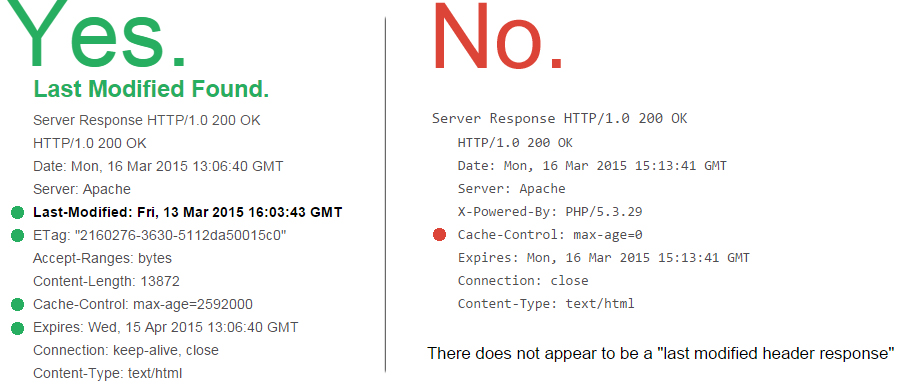
\includegraphics[width=\textwidth]{expires_header.jpg}
		  		\caption{Beispiel: Eine Webseite mit und ohne "`Cache Control"'. (Eigene Abbildung nach feedthebot.com)}
		  		\label{fig:expires_header}
		  	\end{center}
		  \end{figure}
		% subsubsection browser_caching_nutzen (end)
		\pagebreak

		\subsubsection{Komprimierung aktivieren} % (fold)
		\label{ssub:komprimierung_aktivieren}
			Nachdem durch das in Punkt \ref{ssub:ressourcen_reduzieren} beschriebene Verfahren die Ressourcen soweit wie möglich verkleinert wurden, können diese vor dem Versenden komprimiert werden.\footnote{Eine ausführlichere Beschreibung über den GZIP Algorithmus und der textbasierter Dokumentkomprimierung ist hier zu finden: \url{http://www.infinitepartitions.com/art001.html}. Für das tiefere Verständnis bietet auch dieses Video von Google: \url{http://tinyurl.com/mfxt5zt}} Das gängigste Komprimierungsprogramm ist GZIP und wird von allen modernen Browsern unterstützt. Je nach Dateigröße können so die zu übertragenden Datenmenge drastisch Reduziert werden. GZIP kann mittels \texttt{.htaccess} Eintrag von Listing \ref{lst:gzip} in Apache aktiviert werden.\footnote{Für andere Server wie zum Beispiel Nginx oder Node.js gibt es auf GitHub fertige Konfigurationen \url{https://github.com/h5bp/server-configs}}. Einträge in die \texttt{.htaccess} Datei sollten nur dann eingesetzt werden, wenn man zum Beispiel ein Shared Hosting verwendet und dadurch keinen direkten Zugang zur Serverkonfiguration hat. Grund dafür ist, dass die Konfiguration von Apache mittels .htaccess den Server verlangsamt.\autocite{apache}

			\begin{lstlisting}[captionpos=b, caption=gzip, label=lst:gzip, language=bash]
				## gzip Compression if availiable
				<ifModule mod_gzip.c>
				mod_gzip_on Yes
				mod_gzip_dechunk Yes
				mod_gzip_item_include file \.(html?|txt|css|js|php|pl)$
				mod_gzip_item_include handler ^cgi-script$
				mod_gzip_item_include mime ^text/.*
				mod_gzip_item_include mime ^application/x-javascript.*
				mod_gzip_item_exclude mime ^image/.*
				mod_gzip_item_exclude rspheader ^Content-Encoding:.*gzip.*
				</ifModule>
			\end{lstlisting}

			Mittels \url{http://www.feedthebot.com/tools/gzip/} lässt sich überprüfen, ob der eigene Server GZIP erlaubt.

			\begin{figure}[htbp]
				\begin{center}
					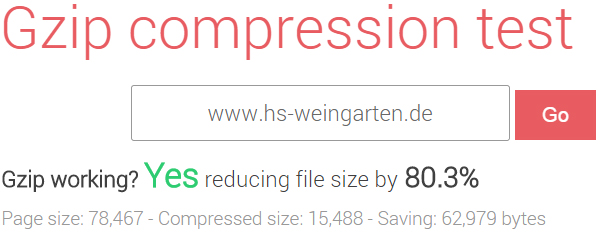
\includegraphics[width=0.5\textwidth]{gzip_compression.jpg}
					\caption{Testen von GZIP anhand von hs-weingarten.de (Eigene Abbildung nach: feedTheBot.com)}
					\label{fig:gzip_compression}
				\end{center}
			\end{figure}
			
			\pagebreak
		% subsubsection komprimierung_aktivieren (end)

		\subsubsection{"`Keep Alive"' ermöglichen} % (fold)
		\label{ssub:keep_alive_ermöglichen}
			Eine weitere Einstellung die in Apache vorgenommen werden kann ist "`Keep Alive"' und hat folgende Bedeutung:
			\begin{quote}
				\textit{"`Webpages are often a collection of many files and if a new connection (the brief communication) has to be opened for each and everyone of those files it could take significantly longer to display that webpage.\\
				More officially the definition of HTTP keep-alive would be something like: a method to allow the same tcp connection for HTTP conversation instead of opening new one with each new request."'}\autocite{sextonAlive}
			\end{quote}

		\begin{lstlisting}[captionpos=b, caption=.htaccess Eintrag nach \autocite{sextonAlive}, label=lst:keepAlive, language=bash]
			## keep-alive
			<ifModule mod_headers.c> 
			Header set Connection keep-alive
			</ifModule>
		\end{lstlisting}
			
		Dieser Eintrag in der .htaccess Datei fügt den \texttt{keep alive header} bei Serveranfragen hinzu.\footnote{Bei shared Hostings kann es trotz dieser Einstellung oft nicht erreicht werden, keep alive zu aktivieren.}
		% subsubsection keep_alive_ermöglichen (end)
		\pagebreak

	% subsection ausgangspunkt (end)

	\subsection{Bilder optimieren} % (fold)
	\label{sub:bilder_optimieren}


		"`Ein Bild sagt mehr als Tausend Worte."' Diesen Spruch gibt es nicht umsonst und auch im modernen Web haben immer mehr und immer größere Bilder Einzug gehalten. Sie werden eingesetzt um eine Botschaft zu übermitteln, Emotionen zu erzeugen oder als \texttt{Eyecatcher}. In Abbildung \ref{fig:site_weight} ist die durchschnittliche Seitengröße der Top 1000 Seiten\footnote{Top 1000 Seiten nach dem Ranking von Alexa: (Alexa gehört zu Amazon und liefert umfassende Analysen über das Web \url{http://www.alexa.com/}) } des Webs abgebildet. So beträgt durchschnittliche die Seitengröße (rechts) zum Zeitpunkt März 2015 rund 1843 kb. Davon sind 65\% (1112 kb) Bildmaterial. Das linke Diagramm zeigt einen Aufwärtstrend der Seitengröße in Kilobyte über die Zeitspanne von einem Jahr. Dabei repräsentiert der Graph in Lila die schlechtesten 90\% der Internetseiten, Grün die 10\% der besten Seiten und Gelb stellt den Median (Mittelwert) dar. Wie zu sehen ist werden die schlechtesten Seiten weiterhin schlechter, indem sie weiter an Kilobytes zulegen, auch der Median und die besten 10\% sind über das Jahr hinweg leicht angestiegen. Mit dem optimieren von Bildern können sehr viele Kilobytes gespart werden.

		\begin{quote}
			\textit{"`Most sites fail to leverage best practices for optimizing images.\\
			Despite the fact that images represent one of the single greatest performance challenges (and opportunities),		34\% of pages failed to properly implement image compression, and 76\% failed to take advantage of progressive	image rendering."'} \autocite[p. 4]{radware14}
		\end{quote}

		\begin{figure}[htbp]
			\begin{center}
				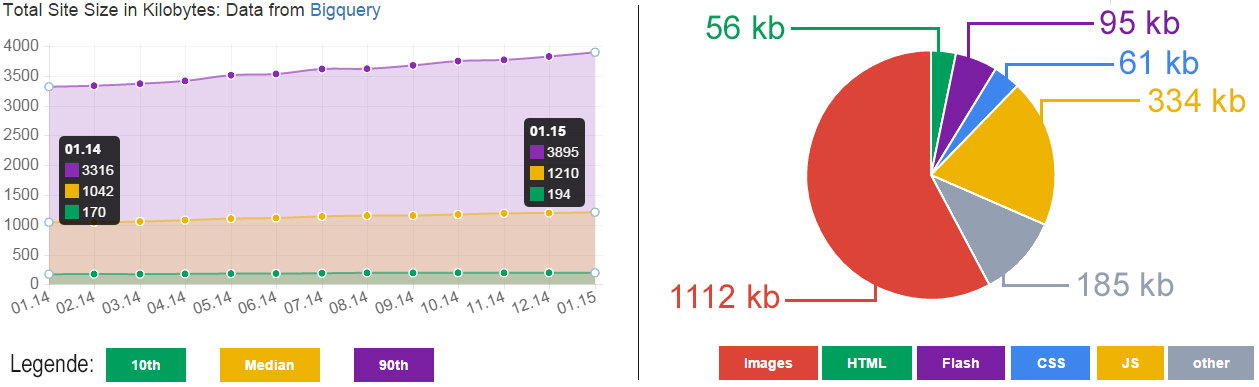
\includegraphics[width=\textwidth]{site_weight2.jpg}
				\caption{Seitenanalyse der populärsten Seiten des Webs (Eigene Abbildung - Daten via \url{bigqueri.es}: Gesamte Auswertung \url{http://tinyurl.com/o8vawxd} )}
				\label{fig:site_weight}
			\end{center}
		\end{figure}

		\subsubsection{Progressive Image Rendering} % (fold)
		\label{ssub:progressive_image_rendering}
			Eigentlich eine sehr alte Technik ist das "`Progressive Image Rendering"'. Es kam längere Zeit außer Mode Bilder als Progressive zu speichern. Der Trend hat sich nun aber wieder geändert und Progressive Images gilt als "`Best Practice"' im Web. Sowohl Webpagetest als auch Google schlagen vor, Bilder Progressive an den Anwender auszuliefern. Testet man eine Seite via Webpagetest.org, so bekommt man unter dem Reiter "`Compress Images"' beispielsweise solch eine Auswertung:
			\begin{quote}
				Use Progressive JPEGs: 100/100\\
				124.8 KB of a possible 124.8 KB (100\%) were from progressive JPEG images
			\end{quote}

			Abbildung \ref{fig:progressive_images} zeigt einmal den normalen Ladevorgang eines Bildes (unten) gegenüber dem "`Progressive Rendering"' (oben).

			\begin{figure}[htbp]
				\begin{center}
					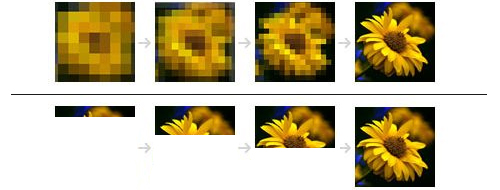
\includegraphics[width=0.7\textwidth]{progressive_images.jpg}
					\caption{Progressives Bilder laden}
					\label{fig:progressive_images}
				\end{center}
			\end{figure}

			Nicht nur sind Progressive Images fast immer ein paar Kilobyte kleiner, sie erhöhen auch die \texttt{Perceived Performance} für den Anwender. Wo bei normalen Bildern lange Zeit eine weiße Lücke klafft, ist bei Progressive Images bereits sehr viel früher das volle Bild zu sehen. Das PNG Äquivalent für Progressive-Jpeg's ist "`Interlaced"'. Bilder sollten zum Beispiel in Photoshop über den Reiter: Datei -> für Web speichern... entweder Progressive oder als Interlaced gespeichert werden.
		% subsubsection progressive_image_rendering (end)

		\subsubsection{Image Spriting} % (fold)
		\label{ssub:image_spriting}
			"`Image Spriting"' bezeichnet das Kombinieren von vielen kleinen Bilddateien zu einer einzigen großen Datei.  Mittels CSS lässt sich aus dem Bild dann das Gewünschte Icon auswählen.

			\begin{figure}[htbp]
				\begin{center}
					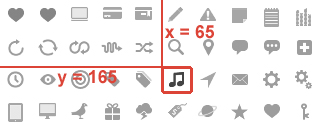
\includegraphics[width=0.6\textwidth]{image_sprites.jpg}
					\caption{Image Sprite von verschiedenen Icons}
					\label{fig:image_sprites}
				\end{center}
			\end{figure}
			
			Der Vorteil dieser Methode ist, dass nur ein Request benötigt wird um alle Icons, die für die Seite benötigt werden, herunterzuladen. Der Nachteil ist, dass durch die Größere Datei der Download länger dauern kann und sich so die Zeit für das erste Rendern verringert. Auch bei einer einzigen Änderung, muss die ganze Datei (die im besten Fall bereits gecached wurde) neu angefragt und ausgetauscht werden.
			
		% subsubsection image_spriting (end)


		\subsubsection{Bild Komprimierung} % (fold)
		\label{ssub:bild_komprimierung}
			Bei der Komprimierung von Bildern unterscheidet man zwischen zwei Arten: "`Lossless"' und "`Lossly"'.
			\begin{itemize}
				\item Lossless bezeichnet die Komprimierung eines Bildes, ohne dabei die Qualität des Bildes zu verändern. So werden bei Lossless zum Beispiel die Metadaten eines Bildes entfernt, die von einer Kamera bei der Aufnahme hinzugefügt werden.
				\item Lossly ist die reduzierung der Bildgröße auf kosten von Qualität. Für die meisten Bilder ist diese Reduzierung aber durchaus Legetim und oftmals sind die Einbußen mit bloßem Auge nicht zu erkennen. Lossly Komprimierung kann aber durchaus bis zu rund 40\% der Bildgröße reduzieren.
			\end{itemize}

			Google hat ein eigenes Bildformat namens "`Webp"' entwickelt und soll bis zu 30\% der Bildgröße bei gleichbleibender Qualität einsparen. Allerdings ist dieses Format nur im Chrome Browser und Opera (der auf Chrome basiert) unterstützt.\autocite{canIuse}

			Eine bessere Alternative ist moz-jpeg. Das ist ein von Mozilla entwickelter JPEG Bild Encoder um die Bildgröße ohne Qualitätseinbußen zu verringern. Dabei bleibt das .jpg Format erhalten und ist somit überall einsetzbar.

			\begin{quote}
				\textit{"`For the short term Mozilla has developed MozJPEG — a modernized JPEG encoder that offers better compression while remaining fully standard-compliant, so it’s compatible with all browsers, operating systems and native apps, and you can use it today without waiting for the whole world to upgrade"'\autocite{mozJPEG}}
			\end{quote}

			Allerdings ist die Verwendung nicht ganz so einfach wie in diesem Zitat dargestellt und es ist das eigenständige Compilieren von \texttt{C}-Code\footnote{Das Repository ist hier zu finden: \url{https://github.com/mozilla/mozjpeg} und eine Anleitung gibt es hier: \url{http://calendar.perfplanet.com/2014/mozjpeg-3-0/}} nötig, um dies auf dem eigenen Betriebssystem zu verwenden.\\
			Glücklicherweise es gibt eine Webanwendung\footnote{Webanwendung zur Verwendung von moz jpeg: \url{https://imageoptim.com/mozjpeg}} mit der ganz einfach per "`drag and drop"' Bilder mittels diesem Encoder komprimiert werden können. Je nach Bild lassen sich so mehrere Hundert Kilobyte einsparen (abhängig von der Qualitätseinstellung und größe des Bildes).\\

			Natürlich bietet auch Photoshop oder IrfanView (Kostenlos) umfangreiche möglichkeiten die Größe von Bildern zu verringern. Moz-jpeg schafft dies allerdings mit einem qualitativ besseren Ergebnis bei zudem kleinerer Bildgröße. Eine Verwendung sollte auf jedenfall in betracht gezogen werden.

		% subsubsection bild_komprimierung (end)

		\subsubsection{Responsive Images} % (fold)
		\label{ssub:responsive_images}
			Bei Bootstrap gibt es die Möglichkeit dem Bild eine Klasse zuzuweisen und das Bild wird dann abhängig von der Fenstergröße skaliert. Genau das steckt aber nicht hinter diesem Begriff. "`Responsive Images"' ist eine auf das Gerät des Endanwenders angepasste Auslieferung von Bildern.\\
			Auf vielen Webanwendungen sieht man folgendes:

			\begin{figure}[htbp]
				\begin{center}
					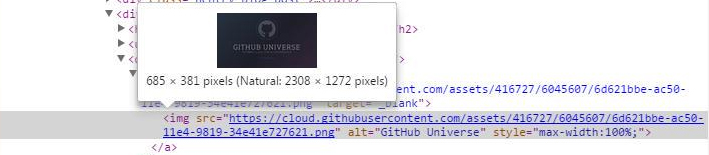
\includegraphics[width=\textwidth]{downsampling.jpg}
					\caption{Downsampling auf GitHub (Eigene Abbildung via Chrome Developer Tool)}
					\label{fig:downsampling}
				\end{center}
			\end{figure}

			Das Bild wurde nicht nur viel zu Groß gewählt, es wird auch auf jedem Gerät, egal ob Tablet, Smartphone oder Desktop die selbe Anzahl an Bytes über die Leitung gesendet. Diese Methode nennt man Downsampling. Das bedeutet, dass nicht das Bild selbst verkleinert wird, sondern der Browser das Bild herunterläd und dann auf die entsprechende Größe skaliert. Das kostet nicht nur Rechenleistung sondern vor allem sehr viel unnötige Bandbreite und sollte unter allen Umständen vermieden werden.\\

			Seit HTML 5 gibt es ein neues HTML Attribut namens \texttt{srcset}. Dieses Attribut ist leider noch nicht in allen Browsern implementiert, hat aber immerhin bereits eine Globale Abdeckung von rund 50\% \autocite{canIuse}. Für dieses Problem gibt es allerdings abhilfe. Es gibt ein Polyfill \footnote{\textit{"`Ein Polyfill [...] ist ein - meist in Javascript geschriebender - Code-Baustein, der in älteren Browsern eine neuere, von diesen nicht unterstützte Funktion mittels eines Workarounds nachrüsten soll. Beispielsweise sind Features von HTML5 in älteren Browsern nicht verfügbar. Webseiten können diese Funktionen trotzdem verwenden, wenn sie ein entsprechendes Polyfill mitliefern."'}\autocite{wikipediaPolyfill}} namens "`Picturefill"'\footnote{Das offizielle Picturefill Projekt ist hier zu finden: \url{http://scottjehl.github.io/picturefill/}}, dass genau diese Funktionalität für alle Browser zur Verfügung stellen kann. Nötig ist dazu nur das herunterladen und Einbinden des Skripts in das HTML Dokument. Dadurch wird folgendes Listing möglich: 

			\begin{lstlisting}[captionpos=b, caption=Srcset in Verwendung, label=lst:srcset]
			<picture id="hero-image">
		    <source srcset="someImg_lg.jpg" media="(min-width: 1367px)">
		    <source srcset="someImg_md.jpg" media="(min-width: 768px)">
		    <source srcset="someImg_xs.jpg" media="(min-width: 300px)">
		    <img srcset="fallback_md.jpg" alt="Some alt text">
			</picture>
			\end{lstlisting}

			Das bedeutet, dass Smartphones mit einer Breite von > 300px < 768px das Bild "`someImg\_xs"' bekommen. Tablets mit 768px < 1367px bekommen das mittlere Bild und alles was über 1367px ist bekommen die größte Version zu Verfügung gestellt. Falls der Anwender Javascript im Browser deaktiviert, ist es möglich ein \texttt{fallback}-Bild zu setzen (Listing: Zeile 8). Man kann sogar einen Schritt weiter gehen und auch das Bildformat auf entsprechend dem Aufrufenden Gerät anpassen:

			\begin{lstlisting}[captionpos=b, caption=Srcset mit webp, label=lst:srcsetWebp]
			<picture id="hero-image">
		    <source srcset="someImg_lg.webp" type="image/webp" media="(min-width: 1367px)">
		    <source srcset="someImg_lg.jpg" media="(min-width: 1367px)">
		    <source srcset="someImg_md.webp" type="image/webp" media="(min-width: 768px)">
		    <source srcset="someImg_md.jpg" media="(min-width: 768px)">
		    <source srcset="someImg_xs.webp" type="image/webp" media="(min-width: 300px)">
		    <source srcset="someImg_xs.jpg" media="(min-width: 300px)">
		    <img srcset="fallback_md.jpg" alt="Some alt text">
			</picture>
			\end{lstlisting}

			Wie zu sehen ist wurden 3 Zeilen eingefügt, die sich lediglich im Typ unterscheiden. Das bedeutet, dass Anwender mit Chrome Browser das Chrome eigene Bildformat .webp bekommen und alle anderen das normale .jpg Format. Voraussetzung ist natürlich, all diese Bilder in ihren verschiedenen Auflösungen und Formaten anzulegen und bereit zu stellen, was einen Mehraufwand bedeutet.
			Picturefill ermöglicht es, Downsampling zu vermeiden und einen auf das Gerät angepasste Version des Bildes auszuliefern. Dadurch sinkt die Anzahl von Bytes die Übertragen werden müssen enorm.


		% subsubsection responsive_images (end)

		\subsubsection{Adaptive Images} % (fold)
		\label{ssub:adaptive_images}
			Adaptive Images ist ein Skript, das mit Hilfe eines PHP-Skripts und einer .htaccess Datei Bilder auf dem Server automatisch auf die verschiedenen Gerätegrößen zuschneidet. Ruft ein Anwender die Seite auf, Prüft das Skript die Größe des Bildschirms und liefer anschlißend das für ihn passende Bild aus. \footnote{Mehr über dieses Skript ist hier zu finden: \url{http://adaptive-images.com/}}

		% subsubsection adaptive_images (end)
		
	% subsection bilder_optimieren (end)

	\subsection{Prozess der Validierung}
	\label{sub:prozess_der_validierung}
		Bereits zu Beginn des Projekts war es wichtig es messbar zu machen. Dafür wurde zu Beginn eine Testumgebung aufgebaut, mit deren Hilfe die Seite nach ihrer Geschwindigkeit getestet werden kann.

	1089 Testläufe über Webpagtest: Zeiraum: 1 Monat

	\begin{figure}[htbp]
		\begin{center}
			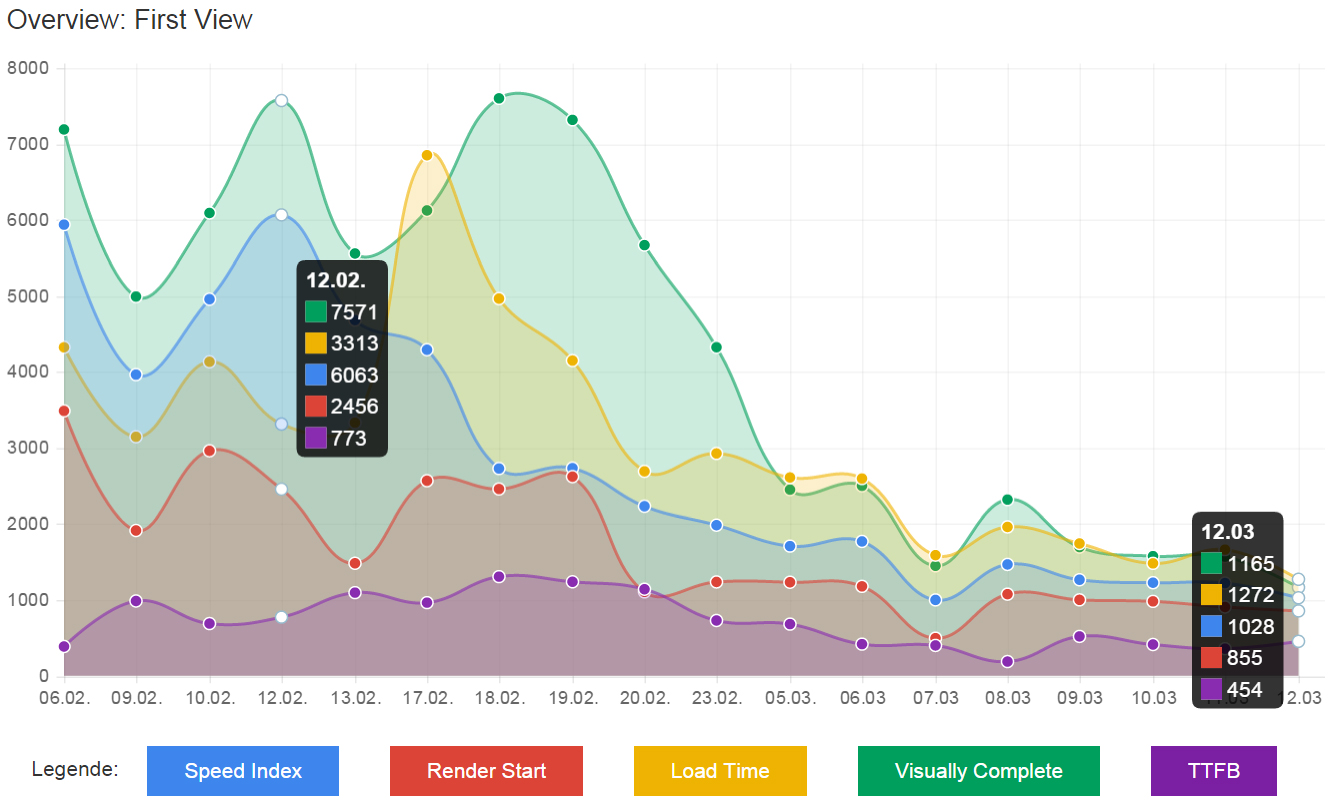
\includegraphics[width=\textwidth]{data_all.jpg}
			\caption{...}
			\label{fig:data_all}
		\end{center}
	\end{figure}
	
	todo
	
	% subsection prozess_der_validierung (end)

	

% section entwicklung (end)
  \section{Workflow} % (fold)
\label{sec:workflow}
	Im folgenden Abschnitt soll erläutert werden wie ein moderner Workflow aussehen kann. Dabei sollen viele Aufgaben, die von vielen noch per Hand erfolgen, automatisiert werden.\\

	\subsection{Nodejs} % (fold)
	\label{sub:nodejs}
		Nodejs - ist eine auf Chromes Javascript runtime aufbauende Plattform. Wärend Server vor allem in PHP oder anderen Sprachen programmiert werden ist dies durch Nodejs auch mit Javascript möglich. Nodejs liefert einen eigenen Paket Manager namens "`npm"'.
	% subsection nodejs (end)

	\subsection{Node Package Manager} % (fold)
	\label{sub:node_package_manager}
		Auch als "`npm"' abgekürzt, erlaubt das installieren von Paketen mittels der Kommandozeile. Ein Beispiel:\\
		Das Paket "`tmi - too many images"' analysiert eine gegebene URL nach ihrer totalen Bildgröße und vergleicht es mit der durchschnittlichen größe des Webs. Es lässt sich mittels \texttt{npm}-Befehl über die Kommandozeile installieren:
		\begin{figure}[htbp]
			\begin{center}
				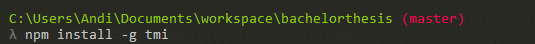
\includegraphics[width=0.7\textwidth]{npm_install.jpg}
				\label{fig:npm_install}
			\end{center}
		\end{figure}
		Danach lässt es sich ganz einfach per Befehl aufrufen:
		\begin{figure}[htbp]
			\begin{center}
				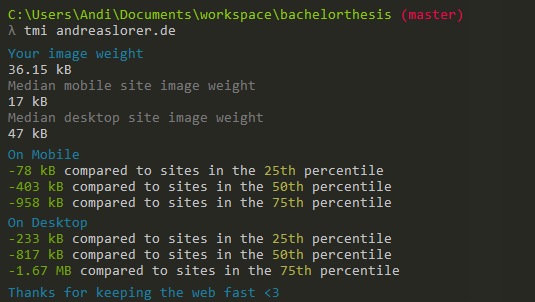
\includegraphics[width=0.7\textwidth]{npm_tmi.jpg}
				\label{fig:npm_tmi}
			\end{center}
		\end{figure}

		Es wäre aber auch möglich das unter Punkt \ref{ssub:google_pagespeed_insight} vorgestellte \texttt{Google Pagespeed Insight} mittels "`npm install -g psi"' zu installieren und per "`psi someURL.de"' aufzurufen. Es gibt bereits mehr als 134,082 Pakete (Stand 21.03.2015) die verschiedenste Aufgaben erledigen können. Das Spektrum an Paketen ist sehr groß und reicht von sinnlosen Aufgaben (wie dem zufälligen generieren von Katzennamen\footnote{Cat-names: \url{https://www.npmjs.com/package/cat-names}}) bis hin zu hoch komplexen Programmen wie "`sitespeed.io"'\footnote{Sitespeed.io: \url{http://www.sitespeed.io/}}, dass eine rekursive Performance-Analyse einer ganzen Webanwendung ermöglicht.\\

		\subsubsection{Dependency Management} % (fold)
		\label{ssub:dependency_management}
			Der klassische Weg wie externe Abhängigkeiten des Projekts geregelt werden sieht wie folgt aus:
			\begin{itemize}
				\item Zu Beginn des Projekts werden Bibliotheken und Frameworks heruntergeladen.
				\item Es folgt das Entpacken und das Verschieben in das richtige Projektverzeichnis.
				\item Erscheint beispielsweise eine neue Version des Frameworks beginnt dieser Prozess von neuem.
			\end{itemize}

			Dependency Manager (wie z.B. npm oder Bower\ref{ssub:bower}) schaffen hier Abhilfe. Durch Ausführen des Befehls: "`npm init"' lässt sich eine neue Abhängigkeitsstruktur für ein Projekt anlegen. Dabei wird eine Datei mit dem Namen: "`package.json"' erzeugt. In dieser Datei werden nun sowohl die Beschreibung, die Version als auch alle Abhängigkeiten gespeichert. Will man nun beispielsweise das Programm "`Gulp"' \ref{sub:task_manager_gulp} installieren, erfolgt dies ganz einfach über das Kommando:\\
			"`npm install -save gulp"'. Die \texttt{-save} Option bedeutet dabei, dass folgender Eintrag in die package.json Datei erfolgen soll:

			\begin{lstlisting}[captionpos=b, caption=, label=lst:]
{
  "dependencies": {
    "gulp": "^3.8.11"
  }
}
			\end{lstlisting}

			\texttt{\textasciicircum 3.8.11} bedeutet dabei, dass für dieses Projekt mindestens eine Gulp Version größer als 3.8.11 vorliegen muss. Der große Vorteil besteht nicht nur darin, dass weder ein Seitenaufruf erfolgt, noch die Dateien entpackt und verschoben werden müssen. Zudem lässt sich über den Befehl "`npm update"' alle Pakete auf die neuste Version bringen. Die package.json Datei lässt sich zudem in die Versionskontrolle einfügen. Der von npm angelegte Ordner: "`node\_modules"' sollte unbedingt per \texttt{.gitignore} von der Versionierung ausgeschlossen werden! Läd ein Teammitglied das Repository herunter, so muss nur noch "`npm install"' aufgerufen werden und alle Abhängigkeiten, mit den für dieses Projekt verwendeten Versionsnummern werden heruntergeladen und installiert. Damit ist jedes Teammitglied auf dem selben Stand und verwenden die selbe Version. Neue Abhängigkeiten lassen sich so auch ganz einfach an alle Mitglieder verteilen.			
			
		% subsubsection dependency_management (end)

		\subsubsection{Bower} % (fold)
		\label{ssub:bower}
			Wie \texttt{npm} so ist auch \texttt{Bower} ein Paket Manager. Um genau zu sein basiert Bower auf npm und lässt sich mittels "`npm install -save bower"' für das Projekt installieren. Der Vorteil von Bower besteht darin, dass über eine \texttt{.bowerrc} Datei angeben werden kann, in welchem Ordner die Pakete installiert werden sollen. Dies ist bei npm nicht möglich.\\
			Es lohnt sich Frameworks und Libraries wie z.B. \texttt{Bootstrap} oder \texttt{Underscore} mittels Bower zu installieren und andere Programme wie zum Beispiel Gulp oder Nodejs Module per npm.\\
			Bower lässt sich, ähnlich wie npm, über das Kommando: "`bower init"' Initialisieren. Danach lassen sich per Befehl "`bower install -save bootstrap"' das Bootstrap Framework installieren. 

			\begin{figure}[htbp]
				\begin{center}
					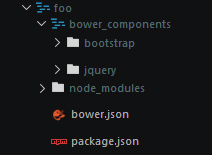
\includegraphics[width=0.3\textwidth]{bower_structure.jpg}
					\label{fig:bower_structure}
				\end{center}
			\end{figure}
			
			Wie zu sehen ist, wurde nicht nur Bootstrap von Bower installiert, sondern auch JQuery. Das liegt daran, dass Bootstrap als interne Abhängigkeit wiederrum auch Abhängigkeiten besitzt, die bei der Installation von Bootstrap gleich mit installiert werden. Entfernt man Bootstrap nun wieder, so würde auch JQuery entfernt werden. Würde Bootstrap in einer neuen Version erscheinen, die von einer höheren JQuery Version abhängt, so würde Bower automatisch auch JQuery auf die nötige Version aktualisieren.
		
		% subsubsection bower (end)

	% subsection node_package_manager (end)

	\subsection{Task Manager - Gulp} % (fold)
	\label{sub:task_manager_gulp}
		Warum braucht es überhaupt einen Task Manager?
		\begin{quote}
			\textit{If you aren't using productivity tools or task automation, you are working \textbf{too hard.} [...] Automation isn't about being lazy. It's about being \textbf{efficient}.}\autocite[p. 18,78]{addyOsmani14}
		\end{quote}
		Ein Task Manger übernimmt immer wiederkehrende Arbeiten. Dazu zählt zum Beispiel die Aufgabe "`minify, uglify und concatenating"' wie in Punkte: \ref{ssub:ressourcen_reduzieren} bereits beschrieben. Aber auch das Übersetzen von "`Sass"'\footnote{Sass is the most mature, stable, and powerful professional grade CSS extension language in the world. \url{http://sass-lang.com}}, das optimieren und verkleinern von Bildern lassen sich als Task beschreiben.
		Die zwei bekanntesten Task Manager heißen \texttt{Gulp} und \texttt{Grunt}. Hier soll das Arbeiten mittels Gulp beschrieben werden, denn er ist sehr viel einfacher zu benutzen als Grunt. Gulp arbeitet nach dem "`stream"' Prinzip:

		\begin{figure}[htbp]
			\begin{center}
				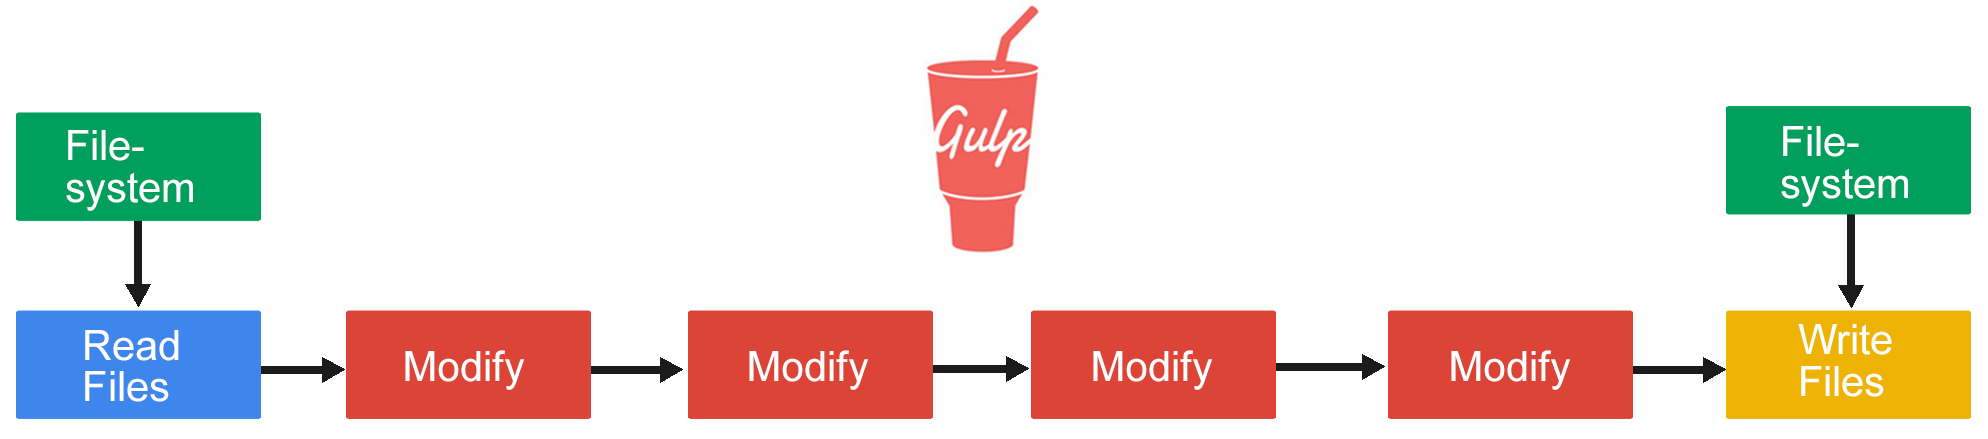
\includegraphics[width=\textwidth]{gulp.jpg}
				\caption{Gulp verwendet streams (Eigene Abbildung nach \autocite[p. 85]{addyOsmani14})}
				\label{fig:gulp}
			\end{center}
		\end{figure}

		Grunt hingegen hat den Vorteil, dass es älter ist als sein Konkurrent (Gulp). Dadurch gibt es viele Pakete, die nur mittels Grunt zur Verfügung stehen. Beispielsweise das Paket "`grunt-responsive-images"'. Damit lassen sich aus einem gegebenen Bild, automatisch verschiedenste Bildgrößen herausrechnen und abspeichern. Dies ist besonders hilfreich, wenn man "`responsive images"' wie in Punkt: \ref{ssub:responsive_images} beschrieben, verwenden möchte.

		\pagebreak
		
		Ein einfacher Task zum Verkleinern von Bildern, zum Beispiel für \texttt{Thumbnails}, kann wie folgt aussehen:
		\begin{lstlisting}[captionpos=b, caption=Ein Simpler Gulp Task zum verkleinern von Bildern, label=lst:gulpResize, breakatwhitespace=false]
		// resize task: resize your images to a given size (e.g 200).
		gulp.task('resize', function () {
		  return gulp.src('site/assets/images/*.jpg')
		    .pipe(imageResize({
		      width : 200,
		      crop : false,
		      upscale : false
		    }))
		    .pipe(gulp.dest('dist/assets/thumbs/'));
		});
		\end{lstlisting}

		Alles was dieser Task macht ist folgendes: Definiere einen Gulp-Task mit dem Namen "`resize"'. Nimm alle Bilder aus dem Ordner "`site/assets/images"'. Verkleinere die Bilder auf 200 Pixel Breite. Speicher die Bilder im Ordner "`dist/assets/thumbs"' ab. Es lassen sich noch viele weitere Tasks schreiben und diese können sich auch gegenseitig aufrufen. 
		

	% subsection task_manager_gulp (end)

	\subsection{Generators}
	\label{sub:generators}
	
	% subsection generators (end)

	\subsection{Minify und Uglify}
	\label{sub:minify_und_uglify}
	
	% subsection minify_und_uglify (end)

	\subsection{Concatenating}
	\label{sub:concatenating}
	
	% subsection concatenating (end)

	

% section workflow (end)
\pagebreak
  \section{Ergebnis} % (fold)
\label{sec:ergebnis}
	Bereits zu Beginn des Projekts war es wichtig es messbar zu machen. Dafür wurde eine Testumgebung aufgebaut, mit deren Hilfe die Seite nach ihrer Geschwindigkeit getestet werden kann. Ganz entscheidend war dabei die Webpagetest API in Verbindung mit Google Spreadsheets. Damit lassen sich regelmäßig automatisierte Tests durchführen und die Daten werden nach erfolgreichem Test automatisch in einer Spreadsheet Tabelle gespeichert. Die über den Zeitraum der Arbeit hinweig gesammelten Daten sind hier finden: \url{http://tinyurl.com/l5usz79}. Diese Daten wurden anschließend mittels \url{http://Chartjs.org} in Diagrammen aufbereitet und alle Diagramme sind auch Online abrufbar unter: \url{http://bithugger.github.io/bachelorthesis/}

	\subsection{Wie wurde getestet?} % (fold)
	\label{sub:wie_wurde_getestet}
		Damit mittels Google Spreadsheets die Webpagetest API verwendet werden kann, ist es nötig einen sogenannten API-Key anzufordern. Ein solcher Key ist kostenlos unter der Adresse: \url{http://www.webpagetest.org/getkey.php} zu erhalten und bietet die Möglichkeit täglich 200 Seitenaufrufe zu tätigen. Als Seitenaufruf zählt sowohl die "`first view"' als auch "`repeat view"'. Die Tests sind 30 Tage abrufbar und gespeichert.\\

		Für das Testen der Seite kann aus einer Vielzahl an Teststandorten gewählt werden. Damit lässt sich nachvollziehen wie beispielsweise die Ladezeiten aus der USA oder Asien sind. Je nach Zielgruppe sollten Tests von verschiedenen Standorten in betracht gezogen werden.\footnote{Eine volle Liste der zur Verfügung stehenden Teststandorte ist im Anhang unter Punkt: \ref{sub:webpagetest_teststandorte} zu finden.} Für dieses Projekt wurden ausschließlich Teststandorte aus der USA und Europa gewählt.\\

		Als Testparameter wurde eine Anzahl von 9 Tests pro Testlauf gewählt. Dabei wurde sowohl die "`first view"' als auch die "`repeat view"' aufgezeichnet. Von den 9 Testläufen wurde der Median als Ergebnis des Testlaufs verwendet. Über den Zeitraum der Arbeit wurde die Seite 1089 Tests unterzogen.\\

		Das größte Problem bestand in der möglichst genauen Messzeiterfassung für die Ladezeiten mittels Smartphone. Webpagetest stellt nur einen Smartphones Teststandort in Dulles USA zu Verfügung. Da die Latenz zwischen dem Hosting in Deutschland und dem Seitenaufruf in der USA sehr viel größer ist, als wenn dieser direkt aus Deutschland erfolgt, wurde nach einer Lösung gesucht diese Messungen exakter zu gestalten.
		Die Lösung dafür ist, ein zweites Hosting mit der selben Seite in den USA zu erstellen. Dafür wurde die "`Microsoft Azure Cloud"' verwendet. Eine kostenlose Testversion ermöglicht es, ganz einfach auf verschiedensten Kontinenten eine Webseite zu hosten. Die Seite wurde für die Tests Online geschaltet und nach den Testläufen wieder Offline genommen.

	% subsection wie_wurde_getestet (end)

	\subsection{Datenauswertung}
	\label{sub:datenauswertung}
		Folgende Daten wurden bei jedem Testlauf erfasst: Speed Index, TTFB (ms), Render start (ms), Visually complete (ms), Dom Content loaded (ms), Site fully loaded (ms), Requests, Bytes in Document.

    Das Diagramm in Abbildung \ref{fig:data_all}, zeigt eine Übersicht der verschiedenen Messwerte über den Zeitraum des Projekts. Die Y-Achse bildet die Zeit in Millisekunden ab und die X-Achse ist das Datum der Messung. Innerhalb von 36 Tagen haben sich alle Werte signifikant verbessert.
    % todo: wirklich 36 Tage? Nachzählen!

    \begin{figure}[htbp]
    	\begin{center}
    		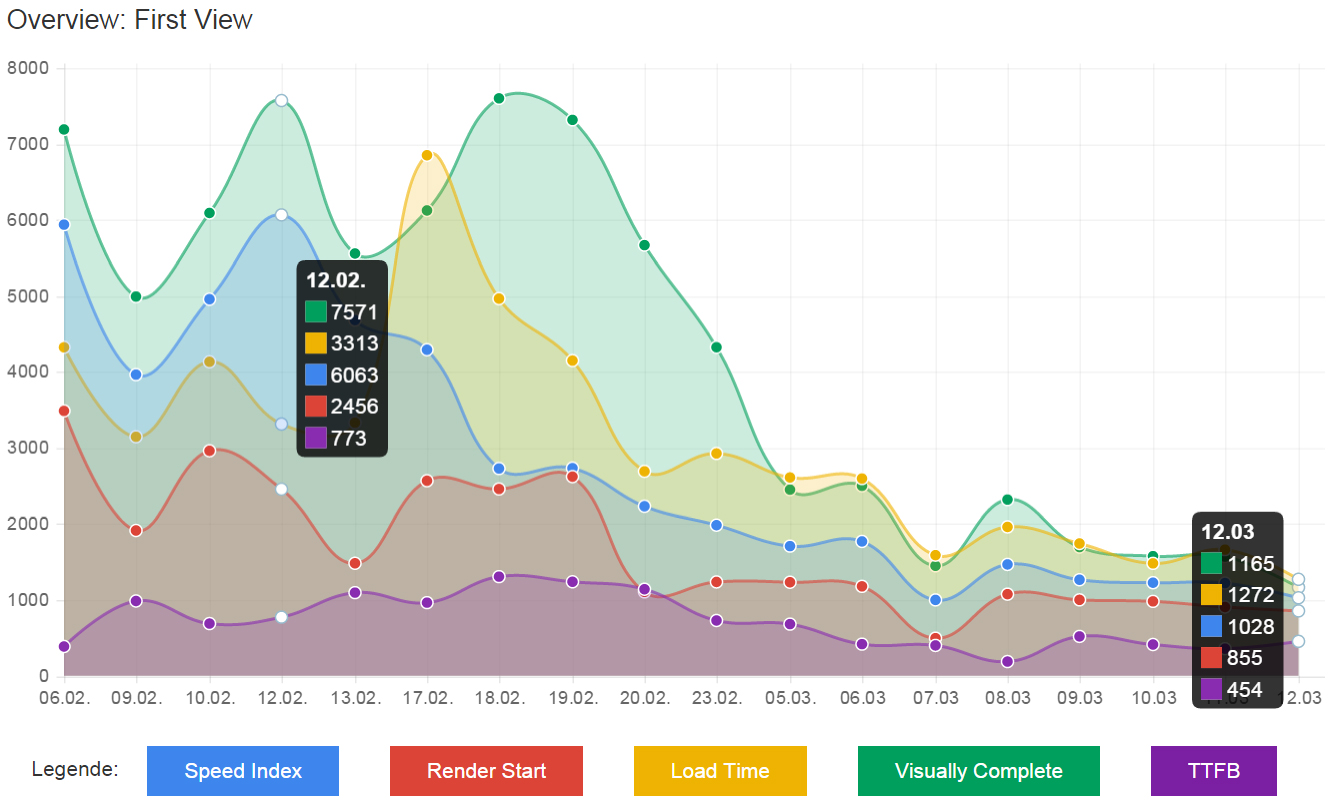
\includegraphics[width=\textwidth]{data_all.jpg}
    		\caption{Datenauswertung - Überblick}
    		\label{fig:data_all}
    	\end{center}
    \end{figure}

    \begin{itemize}
        \item Speed Index: Ein Speed Index von < 1000 Punkten wird als "`schnell genug"' angesehen. Der Median des Speed Indexes konnte von 6063 Zählern auf 1028 Zähler verringert werden. 
        % todo, evt Zitat von Twittter (how fast is fast enough?)
        % fazit: was bedeutet der Speed Index jetzt konkret für den Anwender / Nutzer / fürs Projekt?
        % todo, evt vergleich mit speed index der top 1000 Alexa sites
        \item Render Start: Während dieser Wert bereits bei Projektbeginn mit 2,4 Sekunden für das erste Rendern recht gut war, konnte auch hier fast das dreifache der Zeit (287\%) eingespart werden. Dieser Wert wird durch dieses Diagramm nicht drastisch genug ausgedrückt. So konnte die alte Version der Seite auf dem Smartphone durchaus einen \texttt{Render start} von ganzen 10 Sekunden haben. Das dieser Wert im Diagramm vergleichbar gering ausfällt liegt daran, dass auch viele Tests mittels Desktop PC und Kabelverbindung eingeflossen sind. Die jetzige Renderzeit auf dem Smartphone beträgt ungefähr 1,4 Sekunden. 
        % note: daten, die den render start von 1,4 sec belegen?
        \item Load Time bestimmt, wie lange ein Anwender warten muss, bis eine Interaktion mit der Seite möglich ist. Dieser Wert konnte um volle 2 Sekunden verringert werden. Dies wurde vor allem durch eine verringerung der Seitengröße erreicht.
        % nachprüfen ob das mit der Interaktionszeit so stimmt
        \item Visually Complete: Der höchste Messwert mit rund 7,6 Sekunden konnte auf 1,2 Sekunden verringert werden. Der Hauptgrund dafür ist die Priorisierung des Inhalts "`above the fold"'. Bei der alten Version erfolgte keine priorisierung, welche Bilder zuerst und welche zuletzt geladen werden sollen. Dadurch konnte es sein, dass Bilder die sehr weit unten platziert waren, zuerst geladen wurden was die "`Visually Complete"' Zeit erhöhte. In der neuen Version wird alles, was unterhalb des "`above the fold"' ist verzögert geladen.
        \item TTFB: Dieser Wert ist grundsätzlich nicht beeinflussbar und sollte durch die Wahl des richtigen Hosting Anbieters so niedrig wie möglich gehalten werden.
    \end{itemize}
    \pagebreak

		\begin{figure}[htbp]
			\begin{center}
				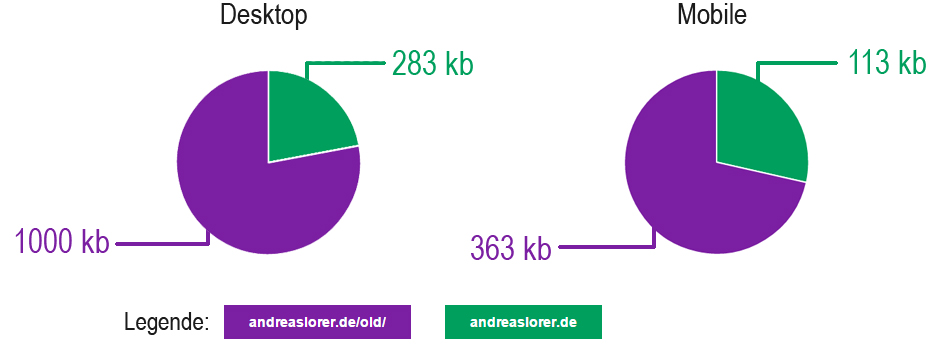
\includegraphics[width=0.8\textwidth]{site_size_in_kb.jpg}
				\caption{Seitengröße in Kilobyte}
				\label{fig:site_size_in_kb}
			\end{center}
		\end{figure}

		Die Seitengröße konnte in der Mobilen und Desktop Variante um rund 3/4 reduziert werden. Dadurch sinkt für den Anwender nicht nur die Ladezeit, sondern auch sein Datenvolumen wird weniger in Anspruch genommen. Laut \url{http://whatdoesmysitecost.com/site/andreaslorer.de} kostet ein Seitenaufruf zwischen 0,01\$ und 0,04\$. Die reduzierung wurde durch mehrere Dinge erreicht: 
		\begin{itemize}
			\item Die "`best practices"' wurden umgesetzt und der Server, wie oben beschrieben, entsprechend konfiguriert.
			\item Bilder "`below the fold"' werden erst dann geladen, wenn der Anwender dort hin scrollt.
			\item Bilder wurden umfassend Komprimiert und \texttt{Progressive} abgespeichert
			\item Das Framework wurde von Bootstrap auf \texttt{Pure.css} gewechselt.
			\item Verwendung von "`Responsive Images"'.
			\item Es werden mittels \texttt{Fontello} nur die Icons geladen, die auch in der Seite eine Verwendung finden.
			\item JQuery wurde als Abhängigkeit für die Bildergallery entfernt. Dadurch kann das herunterladen von JQuery soweit verzögert werden, bis alle wichtigen Teile der Seite geladen wurden. 
			\begin{figure}[htbp]
				\begin{center}
					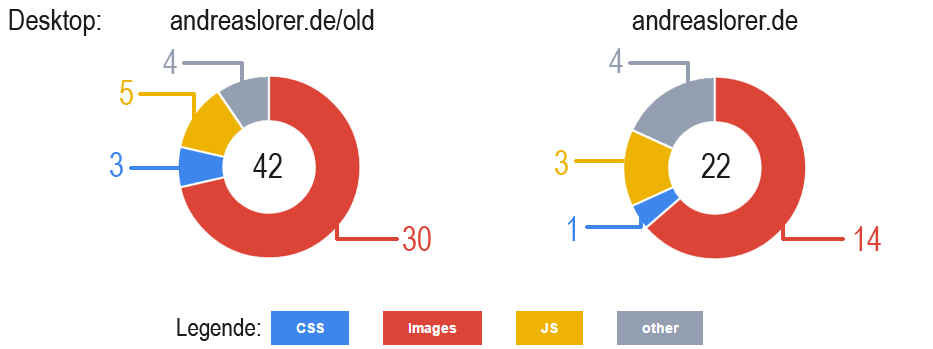
\includegraphics[width=0.8\textwidth]{amount_of_requests.jpg}
					\caption{Anzahl an Requests via Desktop}
					\label{fig:amount_of_requests}
				\end{center}
			\end{figure}
			\item Scripts und sonstige Ressourcen wurden verkleinert und zusammengefasst. Die Anzahl an Requests wurde in der Desktop Variante um die Hälfte verringert.

			\begin{figure}[htbp]
				\begin{center}
					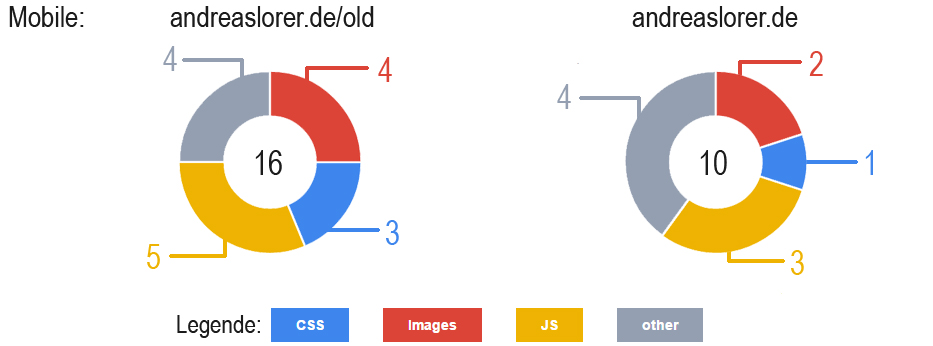
\includegraphics[width=0.8\textwidth]{amount_of_requests_mobile.jpg}
					\caption{Anzahl an Requests via Mobile}
					\label{fig:amount_of_requests_mobile}
				\end{center}
	    \end{figure}

			\item In der Mobilen Variante konnten weitere Requests eingespart werden und es wird nur noch der Hintergrund und das erste Bild der Bildergallery geladen.
		\end{itemize}

		Beim Seitenaufruf mittels Desktop-PC und Kabelverbindung können "`first Render"' Zeiten von unter 189 ms und ein Speed Index von 468 erreicht werden.\footnote{Test Desktop: \url{http://www.webpagetest.org/result/150324_EW_105M/5/details/}} Auf Smartphones mit 3G Netz und 300 ms RTT siehen die Werte etwas schlechter aus und so kann je nach Tag oder Uhrzeit das Ergebnis entsprechend anders ausfallen. Hier sind Werte von 1,3 Sekunden bis zum "`first Render"' und einem Speed Index von 1948 möglich.\footnote{Test Mobile: \url{http://www.webpagetest.org/result/150308_5V_JSD/4/details/}}. Ein visueller Vergleich zwischen der alten und neuen Seite ist in Form eines Videos unter der URL: \url{http://tinyurl.com/o8xoy7m} zu sehen.
		

	% subsection datenauswertung (end)

\pagebreak

%	
% section ergebnis (end)
%


\section{Der Weg zur Performance} % (fold)
\label{sec:der_weg_zur_performance}
	Damit Webanwendungen überhaupt eine gute Performance  bieten können, gibt es eine fundamentale Bedingung: Sowohl das ganze Team als auch das ganze Unternehmen muss hinter dem Gedanken "`Speed is feature number one"'\autocite{holzle10} stehen. Diese Voraussetzung zu erfüllen und alle in ein "`Boot"' zu bekommen kann bereits sehr schwierig sein, ist aber für den Erfolg einer schnellen Webanwendung unabdingbar.

	\begin{quote}
		\textit{"`Performance more often comes down to a cultural challenge, rather than simply a technical one."'} \autocite[p. 13]{kovalcin15}

		\textit{"`If other designers and developers who shape the site aren’t educated on performance, how can they make the best decisions about user experience? How can they weigh the balance between aesthetics and page speed? If they aren’t empowered to make improvements, any performance champions will simply be playing cleanup after other people’s work. Spending your time cleaning up other people’s work (especially when it’s preventable) is a one-way ticket to burnout."'} \autocite{hogan14}
	\end{quote}

	Damit dies gelingt beschäftigt sich dieser Abschnitt mit der Frage, wie der Weg zur Web Performance aussehen kann und welche Hürden es zu meistern gibt.

	\subsection{Hürden} % (fold)
	\label{sub:hürden}
	
	Wenn man an das Thema Web Performance denkt, so mag man in erster Linie denken, dass dies ausschließlich für die Entwickler von Belangen ist.
	
	\begin{figure}[htbp]
		\begin{center}
			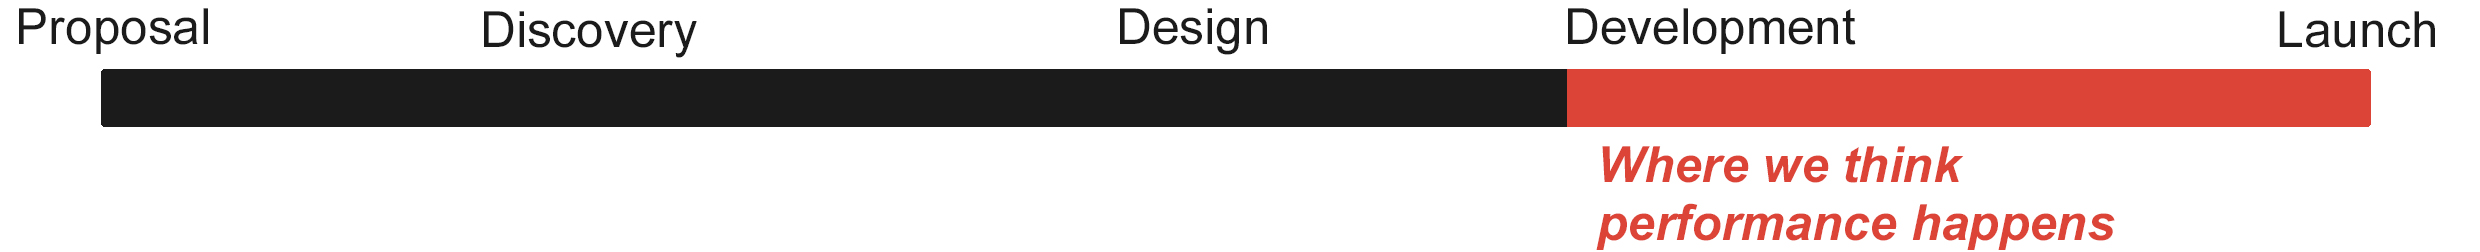
\includegraphics[width=\textwidth]{where_we_think_perf_happens.jpg}
			\caption{(Eigene Abbildung nach \autocite[p. 10]{kovalcin15})}
			\label{fig:where_we_think_perf_happens}
		\end{center}
	\end{figure}

	Genau das Gegenteil ist allerdings der Fall. Wenn eine Webanwendung klassischerweise in die Entwicklungsphase geht, sind bereits die meisten Weichen gestellt. Das Design ist ausgearbeitet und kann mehr oder weniger Mächtig ausfallen. Das Budget für das Projekt wurde vereinbart und der Umfang wurde Vertraglich festgelegt. Das Projektmanagement muss darauf achten, dass die Wünsche und Erwartungen des Kunden erfüllt werden und die Entwicklung sich auf diesen Aspekt konzentriert.

	\begin{figure}[htbp]
		\begin{center}
			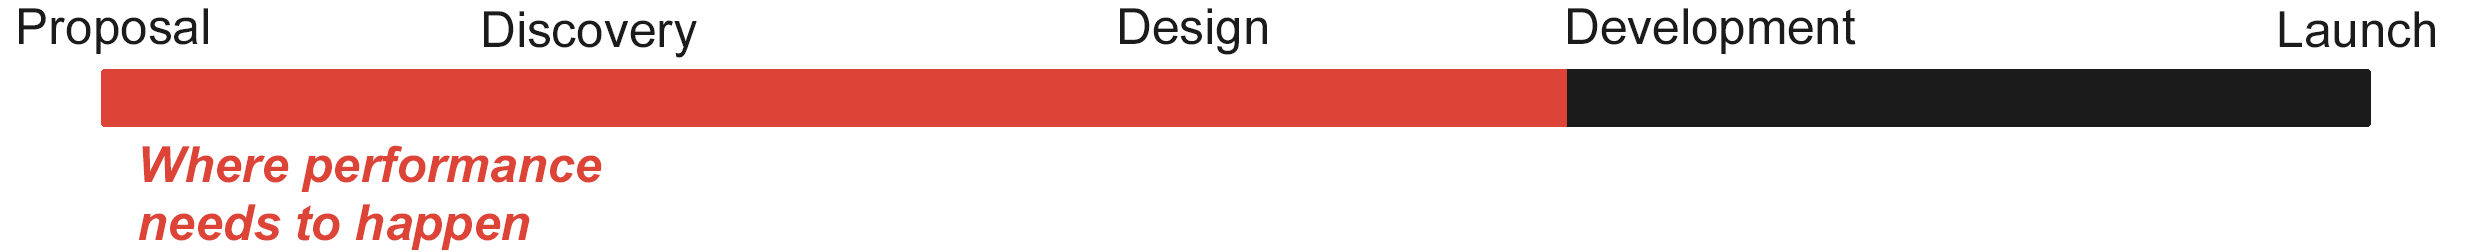
\includegraphics[width=\textwidth]{where_it_needs_to_happen.jpg}
			\caption{(Eigene Abbildung nach \autocite[p. 11]{kovalcin15})}
			\label{fig:where_it_needs_to_happen}
		\end{center}
	\end{figure}

	Deshalb beginnt das Thema Web Performance schon bereits ganz am Anfang. Der Kunde muss mit in das Boot geholt werden und es muss verdeutlicht werden, warum sich schnelle Ladezeiten lohnen, was für negative Auswirkungen langsame und was für positive Auswirkungen schnelle Ladezeiten auf den Endanwender haben. Der Kunde sieht oftmals nicht den Mehrwert an einer schnellen Webanwendung und möchte für etwas, dass er nicht sehen kann auch kein Geld investieren. Argumente wie:
	\begin{quote}
		\textit{"`We surveyed 3000 users about 17 key product drivers. They rated speed 2nd most important only after easy to find content."'} \autocite[p. 8]{hamann14}

		\textit{"`User load time expectations are 2 seconds or less and decreasing"'} \autocite{bixby13}
	\end{quote}
	oder die in dieser Arbeit genannten Argumente können bei der Überzeugungsarbeit helfen.\footnote{Eine Sammlung mit Argumenten ist im Anhang unter Punkt \ref{sub:argumentations_sammlung} zu finden.} Aktuelle Reports oder Zahlen und Fakten die den direkten Zusammenhang zwischen Ladezeit und dem daraus resultierenden Profit verdeutlichen sind, entsprechend aufbereitet, sehr hilfreich.\\
	Der Kunde könnte auch Argumentieren, dass er gar nicht so viele Mobile Anwender hat und es sich deshalb nicht lohnt. Dies war damals die selbe Argumentationsweise, die gegen "`Responsive Webdesign"' sprach. \textit{"`Amongst the top 10,000 websites, almost 8\% of websites went responsive within the span of a single year – an incredible growth!"'}\autocite{guypo14}. Diese Argumentation hielt nicht lange und heute spricht jede Firma von Responsive, will eine Responsive Website oder hat zumindest darüber nachgedacht.\autocite{guypo14} Web Performance ist ein Zukunftstrend, der mit der steigenden Anzahl an Smartphone Nutzer einher geht und damit früher oder später für jeden relevant ist. Ein guter "`sales pitch"' könnte sein:
	\begin{quote}
		 \textit{"`We'll provide you with a \textbf{fast}, responsive, immersive online experience."'}\autocite[p. 32]{kovalcin15}
	\end{quote}
	Dem Kunden muss Performance als visuell greifbares Erlebnis präsentiert werden. Dabei sind nicht nur Diagramme sondern auch Tools wie Webpagetest sehr nützlich. Damit können Vergleichsvideos erstellt werden. Denkbar wäre zum Beispiel ein direkter Vergleich mit den Konkurrenzseiten zu zeigen. Auch ein Vorher- / Nachervergleich eines erfolgreichen Projekts könnte dem Kunden präsentiert werden. Zum Launch kann dann ein Vergleich mit pre- und post-Performance aufgezeigt werden.\\

		\subsubsection{Projekt Manager} % (fold)
		\label{ssub:projekt_manager}
			Für das Team der Projekt Manager ergeben sich laut Katie Kovalcin folgende Hürde: \autocite[p. 43]{kovalcin15}\\
			\begin{itemize}
				\item Understand the importance
				\item Advocate with clients
				\item Help maintain performance budget.
			\end{itemize}
			Zuerst müssen die Projekt Manager verstehen, warum Web Performance wichtig für das Projekt ist um den Kunden entsprechend führen und beraten zu können. Des weiteren muss jemand dafür Sorge tragen, dass das Performance Budget (dazu später mehr) eingehalten wird. Neue Anforderungen und features müssen dementsprechend bewertet und mit dem Kunden diskutiert werden.\\
		% subsubsection projekt_manager (end)

		\subsubsection{Aesthetic heavy designers} % (fold)
		\label{ssub:aesthetic_heavy_designers}
			"`Aesthetic heavy designers"' können oft nicht abschätzen, was ihre Entscheidungen für einen Einfluss auf die Webanwendung haben. Die voraussetzung dafür ist zu wissen, wie das Web funktioniert. Warum Webanwendungen langsam sind und was dazu führt. Erst dann lassen sich Entscheidungen treffen, die sowohl den Endanwender und sein Online Erlebnis, als auch den ästhetischen Anspruch zufriedenstellen. Wikipedia beschreibt den Begriff Design so:

			\begin{quote}
				\textit{"`Insbesondere umfasst Design auch die Auseinandersetzung des Designers \textbf{mit der Funktion eines Objekts sowie mit dessen Interaktion mit einem Benutzer}"'} \autocite{wikipediaDesign}
			\end{quote}

			Design ist also mehr als nur die visuelle Aufbereitung von Informationen, es muss in erster Linie dem Anwender dienen. Webseiten die zu groß sind, zerstören den Ansatz von Web Performance bereits schon zu Beginn. Wie in Punkt \ref{sub:perceived_performance} gesagt, verlassen über 50\% der Nutzer eine Seite nach einer Verzögerung von nur 3 Sekunden. Die emotionsvollsten Bilder und das prächtigste Design kann dem Besucher keine Botschaft vermitteln, wenn sie niemals zu sehen sein werden.

			\begin{quote}
				\textit{"`When you want to be fast, you have to \textbf{give up} the things slowing you down."'}\autocite[p. 2]{osmani14}
			\end{quote}

			Performance darf nicht als schlimmster Feind, sondern muss als bester Freund betrachtet werden. Dabei findet ein Balanceakt statt. Manchmal werden Entscheidungen zugunsten der Performance, ein anderes mal für die Ästhetik getroffen. Der Schlüssel ist es, alle verfügbaren Informationen zu nutzen, um die richtigen Entscheidungen für sich und die Webanwendung zu treffen.\autocite[p. 126]{laraHogan14}\\
			Der Designer muss sich Fragen stellen wie: "`Welchen Mehrwert hat der Nutzer durch dieses große Bild auf der Startseite"', braucht es 3 Schriftarten um einen gewissen \texttt{Look \& Feel} zu vermitteln oder reicht eine? Gibt es eine alternative Schriftart die fast identisch aussehen, aber viel weniger Bytes benötigt? 

			\begin{longtable}{|>{\raggedright \arraybackslash}p{4.9cm}|>{\raggedright \arraybackslash}p{4.9cm}|>{\raggedright \arraybackslash}p{5cm}|}
			\caption{Beispiel: Abwägung - Performance oder Ästhetik  (Tabelle nach \autocite[p. 126]{laraHogan14})}\\
			\hline
				\textbf{Question} & \textbf{Aesthetische Consideration} & \textbf{Performance Consideration}\\
				\hline
				Can I put a large hero image at the top of every page? & Eye-catching represents the brand & This could be a really large file, we want to minimize page weight\\
				\hline
				Should I use three Font-Weights plus a text weight? & Lots of flexibility in typography & We want to reduce page weight and requests\\
				\hline
				Do I need a carousel on the landing page? & Showcases lots of different content & This adds a lot of page weight and additional requests. The user might never see the 2nd image.\\
				\hline
				How can I demonstrate the product functionalities? & Could use a GIF or embed a video & Videos and GIF's can be very heavy.\\
				\hline
			\end{longtable}

			Die Antworten können je nach Projekt oder Designer unterschiedlich ausfallen.

			\begin{longtable}{|>{\raggedright \arraybackslash}p{7.6cm}|>{\raggedright \arraybackslash}p{7.6cm}|}
			\caption{Beispiel: Entscheidungen (Tabelle nach \autocite[p. 127]{laraHogan14})}\\
				\hline
				\textbf{Question} & \textbf{Decision}\\
				\hline
				Can I put a large hero image at the top of very page? & Yes, we use responsive images for the different screen sizes and compress them to reduce page weight! We might lose image quality.\\
				\hline
				Should I use three Font-Weights plus a text weight? & We need the 3 Font-Weights, they are used by the brand. No choice there\\
				\hline
				Do I need a carousel on the landing page? & No the extra images are not increasing the users experience.\\
				\hline
				How can I demonstrate the product functionalities? & We will use CSS-Animations instead of a GIF. This will cost some of the developers time.\\
				\hline	
			\end{longtable}

			Für viele Entscheidungsschritte macht es oft Sinn, dass Entwickler und Designer kollaborieren. Dabei können bereits zu einem sehr frühen Zeitpunkt \texttt{Bottlenecks} erkannt, alterantiven vorgeschlagen und diskutiert werden. Dafür muss es klare Regeln geben. So haben Phrasen wie: "`Das ist zu schwierig, gefällt mir nicht, dumme Idee, da gibt es keine Alternative, das Bild muss genau so aussehen"' generell nichts verloren. Das Wort "`Performance"' darf nicht als \texttt{Trumpfkarte} für einen Entwickler gegenüber dem Designer gesehen werden. Viel mehr Sinn macht es Alternativen zu erarbeiten, Prioritäten zu diskutieren oder Lösungen aufzuzeigen. Ebeneso kann es hilfreich sein, früh mit einem Mockup oder Prototyp auf Code-Basis anzufangen und gemeinsam an diesem auszuprobieren.

			\begin{figure}[htbp]
				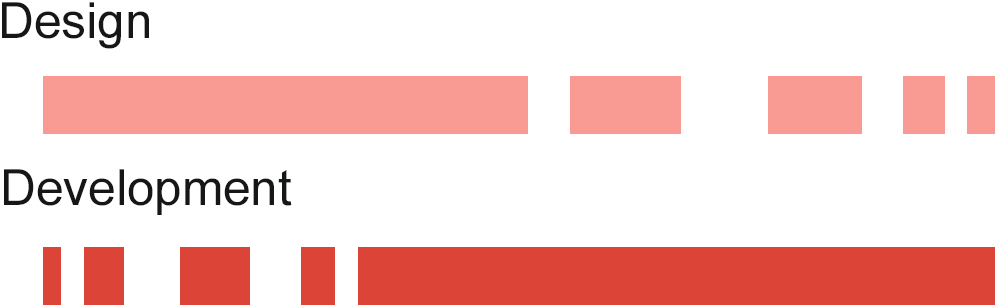
\includegraphics[width=0.5\textwidth]{project_timeline.jpg}
				\caption{Projekt Zeitlinie}
				\label{fig:project_timeline}
			\end{figure}
			
			Auch hier gilt wieder den Balanceakt zwischen Ästhetik und Performance zu finden und nicht gegeneinander, sondern miteinander zu arbeiten. Um dem ganzen einen Rahmen zu geben, in dem sich sowohl Designer, Entwickler als auch der Kunde bewegen darf, wird von vielen Performance Führsprechern ein sogenanntes "`Performance Budget"' verwendet.
		
		% subsubsection aesthetic_heavy_designers (end)
	

	%
	% subsection hürden (end)
	%


		\subsection{Performance Budget} % (fold)
		\label{sub:performance_budget}
			Ein Performance Budget bedeutet, dass ein Wert gesetzt wird, der von der Seite nicht überschritten werden darf. Dieser Wert kann ganz simpel sein, wie die Ladezeit der Seite oder aber eine komplexere Metrik aus verscheidenen Werten.

			\begin{quote}
				\textit{"`The important point is to look at every decision, right through the design/build process, as something that has consequence. Having a pre-defined ‘budget’ is a clear, tangible way to frame decisions about what can and can’t be be included, and at a suitably early stage in the project. It can also potentially provide some justification to the client about why certain things have been omitted (or rather, swapped out for something else)."'}
			\end{quote}

			Die Einführung eines Performance Budgets bietet den Vorteil, einen festgelegten Rahmen über die Zeitspanne des Projekts zu haben. Es ist ein Referenzpunkt der mit darüber Entscheidet, welche und welche Komponenten nicht in die Seite mit einfließen können oder dürfen. Es Funktioniert wie Spielgeld, dass auf das Projekt aufgeteilt wird. Ist das Spielgeld leer, so gibt es diese 3 Regeln:
			\begin{enumerate}
				\item Optimiere eine existierende Funktion der Seite
				\item Entferne eine existierende Funktion von der Seite
				\item Füg es nicht hinzu
			\end{enumerate}
			Das Motto heißt dabei: "`you can't spend, what you don't have!"'

			\subsubsection{Budget Metriken} % (fold)
			\label{ssub:Budget_metriken}
				
				Eine sehr einfache Budget Metrik währe es, den Speed Index als Budget zu setzen. Jede Seite muss dann unter diesem festgelegten Wert bleiben. Oftmals ist es aber besser verschiedene Werte als Budget zu setzen. Eine Kombination aus: Anzahl Requests, start Render, maximale Seitengröße, maximales Gewicht der Bilder und zusätzlich der Speed Index können eine sinnvolle und verständliche Basis bilden. Es können aber je nach Projekt auch anwendungsbezogene Metriken verwendet werden. So benutzt Twitter zum Beispiel die Metrik "`Time to first Tweet"'.

				\begin{quote}
					\textit{"`The most important metric we used was “time to first Tweet”. This is a measurement we took from a sample of users, of the amount of time it takes from navigation (clicking the link) to viewing the first Tweet on each page’s timeline. The metric gives us a good idea of how snappy the site feels."'} \autocite{twitter12}
				\end{quote}

			% subsubsection Budget_metriken (end)

			\subsubsection{Wie schnell, ist schnell genug?} % (fold)
			\label{ssub:wie_schnell_ist_schnell_genug_}
				Wie wird das Performance Budget gesetzt? Dazu ist es erforderlich zu wissen, wie schnell eigentlich schnell genug ist? Schnelligkeit ist ein relativer Begriff.

				\begin{quote}
					\textit{"`In the high-speed world of automated financial trading, milliseconds matter. So much so, in fact, that a saving of just \textbf{6 milliseconds} in transmission time is all that is required to justify the laying of the first transatlantic communications cable for 10 years at a cost of more than \$300m between London and the New York Wall Street."'} \autocite[vgl.]{telegraph11}
				\end{quote}

				Aber auch Google stellt fest, dass bereits der Einfluss von nur \textbf{100 - 400 ms} einen messbaren Einfluss auf die Anzahl an Suchanfragen (-0,2\% bis -0,6\%) pro Anwender hat.\autocite{google09} Während 0,4\% sich nach wenig anhört, so ist bei jährlich 2,2 Billionen Suchanfragen (2013) wohl klar, was das für Google an Mehreinnahmen durch Werbung und Klicks bedeuten kann.\autocite{statista14}\\
					
				Studien haben ergeben, dass Menschen den Unterschied zwischen 2 Zeitspannen erst dann erkennen, wenn die Differenz 20\% überschreitet.\autocite{seow09} Damit der Anwender eine Verbesserung gegenüber der Konkurrenz bemerkt, benötigt es in Folge dessen mindestens einen 20 prozentigen Unterschied. Anhand der Konkurrenzanalyse lässt sich ein Ergebnis bestimmen, mit dessen Hilfe das Performance Budget festgelegt werden kann. Bei einem \texttt{Relaunch} kann auch die alte Seite als Refernzpunkt dienen.\\
				Zu beachten bleibt, die Daten richtig zu interpretieren. Eine Seite die eine 7 Sekunden Ladezeit hat muss nicht unbedingt langsamer sein (Stichwort: Perceived Performance) als eine Seite mit 5 Sekunden. Hier lohnt sich vor allem die Beachtung des Speed Indexes, der die Seite nach dem "`visuellen Fortschritt über Zeit"' bewertet. Die 20\%-Methode liefert den wohl minimalsten "`schnell-genug"' Wert der erreicht werden sollte, um sich von der Konkurrenz abzusetzen.\\
				Paul Irish, Mitarbeiter des Google Chrome Teams, sieht das ganze drastischer und gibt folgendes Statement:
				\begin{quote}
					\textit{"`My answer to how fast is fast enough? A Speed Index of under 1000.\\
					And for professionals that get there, they should shoot for delivering the critical-path view (above the fold) in the first 14kb of the page."'} \autocite{irish14}
				\end{quote}
				Für viele (vor allem im Bereich des E-Commerce) kann es sich rechnen, nicht nur schneller als die Konkurrenz zu sein.
			% subsubsection wie_schnell_ist_schnell_genug_ (end)

		\subsubsection{Arbeiten mit einem Performance Budget} % (fold)
		\label{ssub:arbeiten_mit_einem_performance_budget}
			Im folgenden soll Beispielhaft verdeutlicht werden, wie das Arbeiten mittels Performance Budget aussehen kann. Zu Projektbeginn wird das Performance Budget festgelegt.

			\begin{figure}[htbp]
				\begin{center}
					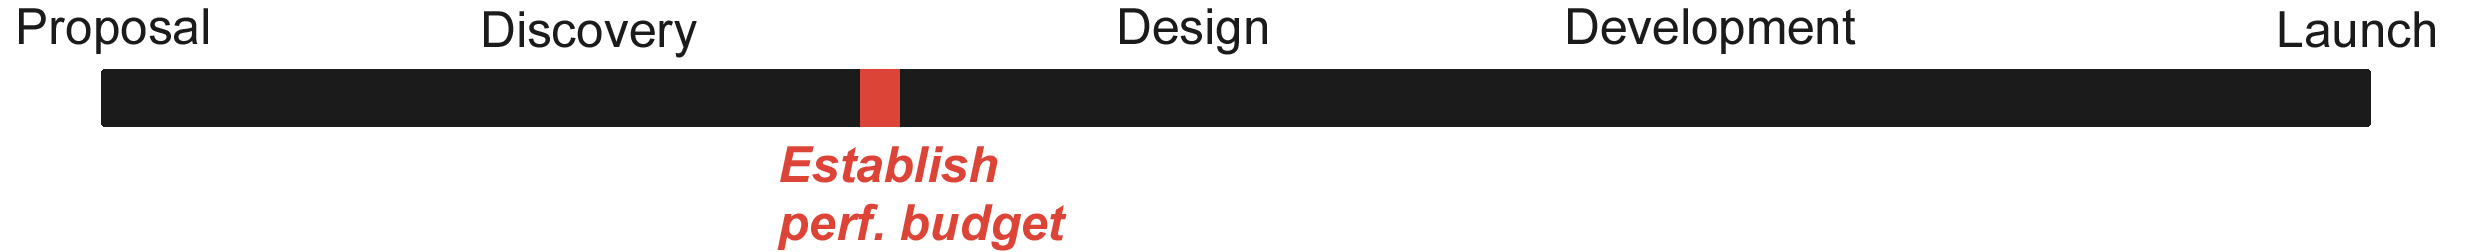
\includegraphics[width=\textwidth]{establish_perf_budget.jpg}
					\caption{Projekt Zeitline (Eigene Abbildung nach \autocite[p. 58]{kovalcin15}}
					\label{fig:establish_perf_budget}
				\end{center}
			\end{figure}
			
			Vor Projektbeginn macht Sinn, denn hat die Seite erst einmal 3 Slider, 1 Karousel plus entsprechendes Plugin und zudem noch ein vollflächiges Hintergrundbild, so hat man keine Chance mehr die Seite in einen geordneten Rahmen zu bringen, ohne sie komplett neu zu überarbeiten.\\
			Ein Beispiel Budget kann aus folgenden Metriken bestehen:

			\begin{itemize}
				\item Maximale Seitengröße 600 kb
				\item Start Render 1000 ms
				\item Speed Index 1000
			\end{itemize}

			Die Seitengröße lässt sich nun aufteilen:
			\begin{longtable}{|>{\raggedright \arraybackslash}p{3.0cm}|>{\raggedright \arraybackslash}p{3.0cm}|}
			\caption{Seitengröße mit einem Budget von 600 kb}\\
				\hline
				\textbf{Content} & \textbf{Size}\\
				\hline
				CSS & 50 kb\\
				\hline
				Fonts & 50 kb\\
				\hline
				Scripts & 100 kb\\
				\hline
				Images & 400 kb\\
				\hline
			\end{longtable}

			Mit diesem Budget ist festgelegt, wieviel Spielraum jede Komponente hat. Will man 500 kb den Bildern zu Verfügung stellen, so muss in den anderen Bereichen eingespart werden. Dieses Beispiel verdeutlicht den Ansatz: "`You can't spend what you don't have"'.\\

			Nachdem das Budget festgelegt wurde ist sowohl das Design, die Entwicklung als auch das Projektmanagement damit beauftragt, das Budget beizubehalten.

			\begin{figure}[htbp]
				\begin{center}
					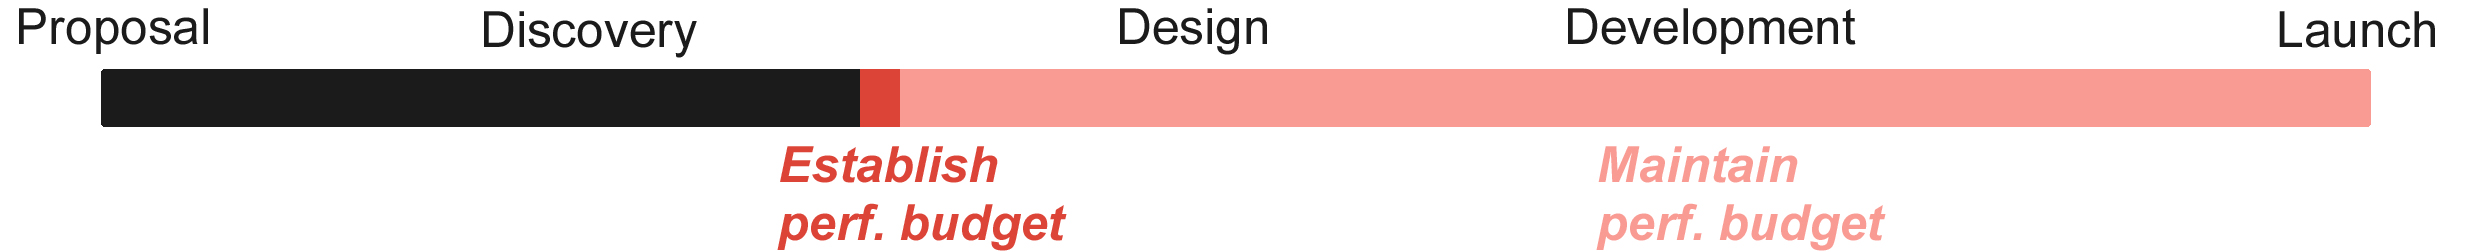
\includegraphics[width=\textwidth]{perf_budget.jpg}
					\caption{Projekt Zeitline (Eigene Abbildung nach \autocite[p. 59]{kovalcin15})}
					\label{fig:perf_budget}
				\end{center}
			\end{figure}

			Dafür muss dem Kunden vermittelt werden, um was es sich bei diesem Budget handelt und warum es verwendet wird: (Aufzählung nach \autocite[p. 72]{kovalcin15})

			\begin{itemize}
				\item Was ist ein Performance Budget?
				\item Was ist das Performance Budget für dieses Projekt?
				\item Was sind die Bedingungen für dieses Budget?
				\item Warum wird es verwendet?
				\item Wie werden neue Funktionen hinzugefügt? (Optimieren, entfernen, nicht hinzufügen)
				\item Wieviel Budget hat jede Seite- / Unterseite
			\end{itemize}

			Für Designer (als auch Entwickler) ergibt sich ein Rahmen. Dies muss in keiner Weise schlecht sein und Dan Mall, Art Director und Designer sagt dazu folgendes:

			\begin{quote}
				\textit{"`I believe designers do their best work within constraints, \textbf{and knowing those constraints before starting a design can be incredibly enabling}. What I wouldn’t give to know that I could use up to 10 images and 4 webfonts before starting a design! What a day that would be! Here’s how to make that possible. [We define a Performance Budget]"'}\autocite{mall14}
			\end{quote}

			Wenn diese Weichen für das Projekt gestellt wurden, dann kann das Entwickler-Team die Anwendung im Sinne der Performance umsetzen.\\
			Mittels Grunt (leider gibt es noch keine gute Gulp Alternative) lässt sich ein npm Paket namens "`Grunt perfbudget"' installieren. Dieses ermöglicht es für die Seite einen Budget Task festzulegen. Dieser Task kann nun in den \texttt{Build-Prozess} der Seite integriert werden. Wird das Budget überschritten, so würde der \texttt{Build-Task} fehlschlagen.

			\begin{figure}[htbp]
				\begin{center}
					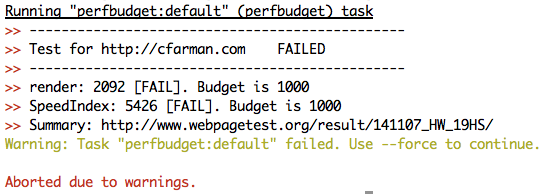
\includegraphics[width=0.7\textwidth]{perf-budget.png}
					\caption{Fehlschlagender Grunt Budget Task (Abbildung von \autocite{farman14})}
					\label{fig:perf-budget}
				\end{center}
			\end{figure}
		
		Das setzen eines Performance Budget und das Arbeiten damit, ist eine Herausforderung. Das Budget unterscheidet sich je nach Projekt und es kann schwierig sein die richtigen Metriken festzulegen. Dieser Abschnitt hat auch gezeigt, dass Web Performance nicht abhängig von einem einzigen Entwickler ist, sondern kann nur gelingen, wenn alle an einem Strang ziehen.	
		% subsubsection arbeiten_mit_einem_performance_budget (end)

	% subsection performance_budget (end)

\pagebreak
%
% section der_weg_zur_performance (end)
%

  \section{Ausblick} % (fold)
\label{sec:ausblick}
	Sowohl für die Endanwendner als auch für die Entwickler und Designer, hat die Zukunft vor allem positive Änderungen für sich parat. Das Http/1.1 Protokoll wird durch Http/2.0 abgelöst. Der LTE-Netzausbau schreitet weiter voran, deckt dabei eine immer größere Fläche ab und bringt den Nutzern damit eine niedrigere Latenz und eine höhere Bandbreite. Auf der diesjährigen Cebit wurde der neue Mobilfunkstandard \texttt{5G} von Vodafone präsentiert. Dieser steht noch in der Entwicklung, wird aber für das Jahr 2020 für den komerziellen Einsatz vorhergesagt. 5G soll dabei Latenzen zwischen 1 bis 10 Millisekunden liefern und eine 100 mal höhere Bandbreite von bis zu 10.000 MBit/s zur Verfügung stellen.\autocite{lte-anbieter15} Ob diese Geschwindigkeiten auch wirklich innerhalb von nur 5 Jahren erreicht werden können, oder ob sie in erster Linie nur der \texttt{PR} dienen, bleibt dabei abzuwarten.

	\subsection{Http/2.0} % (fold)
	\label{sub:http_2_0}
		\begin{figure}[htbp]
			\begin{center}
				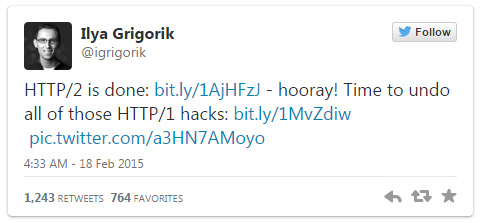
\includegraphics[width=0.6\textwidth]{http2_done.jpg}
				\caption{Http 2.0 wurde veröffentlicht}
				\label{fig:http2_done}
			\end{center}
		\end{figure}

		Dieses Jahr ist es soweit und das Http/1.1 Protokoll aus dem Jahre 1999 wird durch Http/2 abgelöst. Natürlich verschwindet das alte Protokoll nicht von heute auf morgen. Http/1.1 wird noch viele Jahre erhalten bleiben, vielleicht auch nie gänzlich verschwinden. Dennoch sagt Daniel Stenberg, Mitglieder der Http/2 Work Group, voraus, dass bis Ende 2015 der Anteil an Http/2 traffic mehr als 10\% beträgt.\autocite{stenberg15} Die großen Browser Chrome und Firefox haben in ihrer aktuellen Version Http/2 bereits aktiviert und auch der Internet Explorer soll mit Windows 10 (in der \texttt{Technical Preview} bereits aktiv) Http/2 unterstützen.\autocite{microsoft14} Schlusslicht bildet Apple mit seinem Safari Browser, von denen bis Dato (01.04.2015) noch keine Stellungnahme zu Http/2 verlautet wurde.
		Die zwei weitverbreitesten Server Apache und Nginx sind dabei, Http/2 zur Verfügung zu stellen. Apache hat bereits ein Http/2 Modul in der Alpha Phase. Nginx sagt, dass sie bis Ende 2015 Http/2 unterstützen werden.\\
		Google (damit auch Youtube und andere Produkte die zu Google gehören) und Twitter haben bereits Http/2 seit einigen Monaten aktiviert.

		\begin{figure}[htbp]
			\begin{center}
				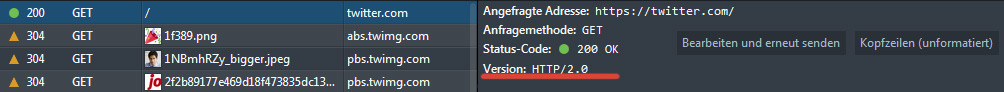
\includegraphics[width=\textwidth]{http2.jpg}
				\label{fig:http2}
			\end{center}
		\end{figure}

		Http/2 bietet folgende Performance Verbesserungen:

		\begin{itemize}
			\item Parallel Multiplexing anstatt der Verwendung von Parallelen Verbindungen
			\item Verwendet nur eine einzige TCP Verbindung
			\item Server-Push
		\end{itemize}
		
		\subsubsection{Http/1.1 Optimierungen in Http/2} % (fold)
		\label{ssub:http_1_1_optimierungen_in_http_2}
			Viele Optimierungs Pattern für Http/1.1 stellen sich für das Http/2 Protokoll als Anti-Pattern heraus. Http/2 bringt den Vorteil, dass es genau eine TCP Verbindung benötigt. Damit wird \texttt{Domain Sharding} ein Performance Anti-Pattern für HTTP 2.0. Auch die Verwendung von \texttt{Image Sprites}, das Zusammenfügen von CSS und Javascript zu einer Datei ist ein Anti-Pattern wenn Http/2 verwendet wird. Eine Vielzahl von kleinen einzelnen Dateien werden zu keinem Performance Problem mehr durch Http/2.\autocite{grigorikHttp2}\\
			"`Server Push"' ist eine Mechanik, die in Http/1.1 durch das Inlinen von CSS in das HTML Dokument bereits simuliert wird. De facto ist dies ein Workaround für eine Funktionalität die nun durch Http/2 bereitstellt wird. Durch Inlinen wird bei einer Anfrage gleich das CSS / Javascript als Antwort mitgesendet, dass der Browser zur Darstellung des "`above the fold"' Inhaltes braucht.

			\begin{figure}[htbp]
				\begin{center}
					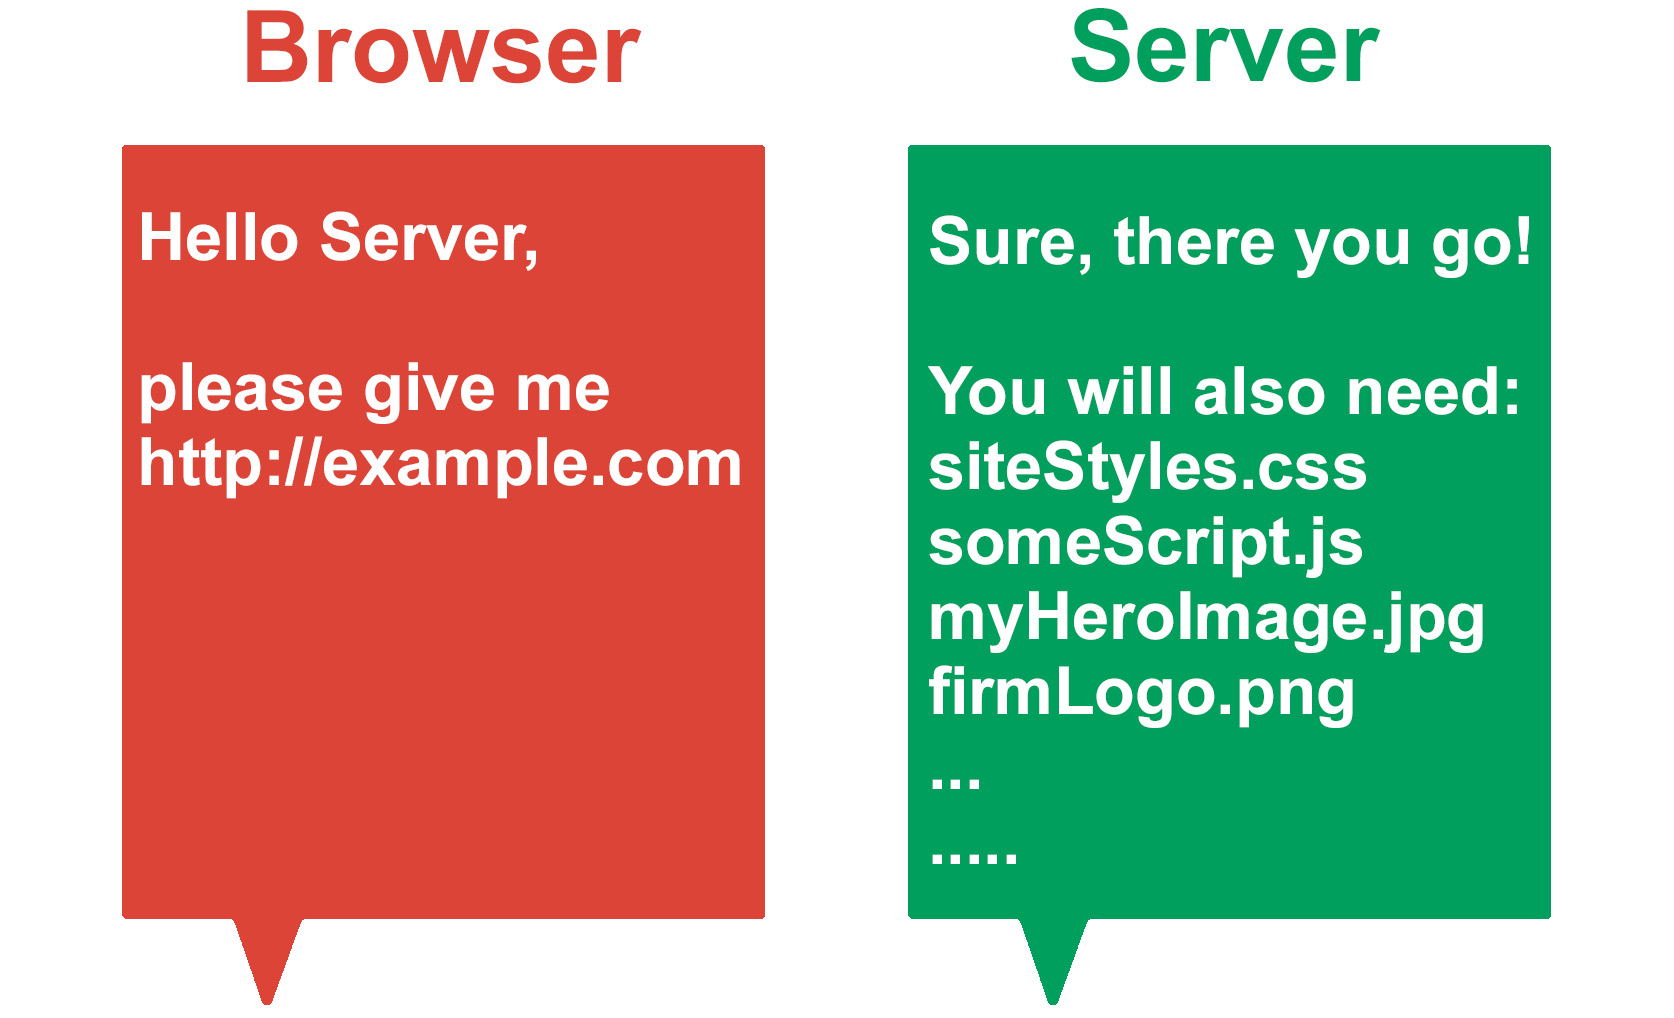
\includegraphics[width=0.6\textwidth]{server_push.jpg}
					\caption{Veranschaulichung der Server Push Mechanik (Eigene Abbildung)}
					\label{fig:server_push}
				\end{center}
			\end{figure}
			
			Durch \texttt{Server Push} wird genau dies möglich, ohne es Inline in das Dokument zu schreiben. Dadurch sind die Ressourcen vom Browser im Cache speicherbar und können auch in den Unterseiten verwendet werden. Bereits bevor der Anwender die Seite besucht, weißt man welche Ressourcen ihm zur Verfügung gestellt werden müssen, um die Seite anzuzeigen. Diese Ressourcen lassen sich somit gleich auf die erste Anfrage als Antwort mitsenden und es wird damit das Explizite \texttt{Anfragen und Antworten} eingespart.\footnote{Dieses Video stellt eindrücklich die Auswirkung der Server Push Mechanik vor (Länge 5 Minuten): \url{https://youtu.be/4Ai_rrhM8gA?t=29}}\\

			Durch Http/2 ergeben sich viele Vereinfachungen, aber auch neue Herausforderungen. Der Umstieg von Http/1.1 auf Http/2 wird nicht über Nacht geschehen. Für viele Seitenbetreiber wird es deshalb nötig sein, sowohl auf das Alte, wie auch das neue Protokoll zu optimieren und an den jeweiligen Anwender die jeweils richtige Version auszuliefern. Dafür gibt es mehrere Ansätze und eine ausführliche Beschreibung dazu gibt es hier: \url{http://tinyurl.com/phnq5d9}. \footnote{Eine detailierte Erklärung zu Http/2.0 ist dem PDF: http2 explained - Daniel Stenberg: \url{http://daniel.haxx.se/http2/http2-v1.11.pdf} zu entnehmen.}

		% subsubsection http_1_1_optimierungen_in_http_2 (end)

	% subsection http_2_0 (end)

\pagebreak
%
% section ausblick (end)
%


\section{Fazit} % (fold)
\label{sec:fazit}
	Restate the Topic
	Restate the Thesis
	Summarize your main Points
	Call to Action (optional)


	Is the web getting faster?
	Warum bedeutet diese Arbeit etwas? 
	Whats your final point you wanna make?
	Was ist das große Ganze der Arbeit?

% section fazit (end)

  \section{Anhang} % (fold)
\label{sec:anhang}

	\subsection{Webpagetest Teststandorte} % (fold)
	\label{sub:webpagetest_teststandorte}

		\begin{tabular}[pht]{lll}
		  Name && Standort \\ \hline
			Eu-West, Chrome, Cable && ec2-eu-west-1:Chrome \\[8pt]
			Eu-West, Chrome, 3G	&& ec2-eu-west-1:Chrome.3G \\[8pt]
			Eu-Central, Firefox	&& ec2-eu-central-1:Firefox \\[8pt]
			Dulles, MotoG, Chrome &&	Dulles\_MotoG:Motorola G - Chrome \\[8pt]
			Us-East, Chrome, 3G	&& ec2-us-east-1:Chrome.3G \\[8pt]
			Eu-Central, Chrome	&& ec2-eu-central-1:Chrome.3G \\[8pt]
			Eu-Central, IE\_11	&& ec2-eu-central-1:IE 11 \\[8pt]
			Us-East, IE11	&& ec2-us-east-1:IE 11 \\[8pt]
			Us-East, Firefox	&& ec2-us-east-1:Firefox \\[8pt]
			Us-West, Chrome	&& ec2-us-west-1:Chrome \\[8pt]
			Us-West, IE11	&& ec2-us-west-1:IE 11 \\[8pt]
			Us-West, Firefox	&& ec2-us-west-1:Firefox \\[8pt]
			Us-West-2, Chrome	&& ec2-us-west-2:Chrome \\[8pt]
			Us-West-2, IE\_11	&& ec2-us-west-2:IE 11 \\[8pt]
			Us-West-2, Firefox	&& ec2-us-west-2:Firefox \\[8pt]
			Ap-Northeast, Chrome	&& ec2-ap-northeast-1:Chrome \\[8pt]
			Ap-Northeast, IE\_11	&& ec2-ap-northeast-1:IE 11 \\[8pt]
			Ap-Northeast, Firefox	&& ec2-ap-northeast-1:Firefox \\[8pt]
			Ap-Southeast-1, Chrome	&& ec2-ap-southeast-1:Chrome \\[8pt]
			Ap-Southeast-1, IE\_11	&& ec2-ap-southeast-1:IE 11 \\[8pt]
			Ap-Southeast-1, Firefox	&& ec2-ap-southeast-1:Firefox \\[8pt]
			Ap-Southeast-2, Chrome	&& ec2-ap-southeast-2:Chrome \\[8pt]
			Ap-Southeast-2, IE\_11	&& ec2-ap-southeast-2:IE 11 \\[8pt]
			Ap-Southeast-2, Firefox	&& ec2-ap-southeast-2:Firefox \\[8pt]
			SA-East, Chrome	&& ec2-sa-east-1:Chrome \\[8pt]
			SA-East, IE\_11	&& ec2-sa-east-1:IE 11 \\[8pt]
			SA-East, Firefox	&& ec2-sa-east-1:Firefox \\[8pt]
		\end{tabular}


	% subsection webpagetest_teststandorte (end)

% section anhang (end)
	\pagebreak

	\printbibliography

\end{document}